\documentclass[12pt,a4paper,titlepage]{article}
% Daniel Wong December 28, 2019

\usepackage[fleqn]{amsmath} % To write aligned equations
\usepackage{amssymb} % To write math symbols
\usepackage{graphicx,float} % To add pictures
\usepackage{caption} % To add captions
\usepackage{subcaption} % To add subcaptions
\usepackage{multirow} % To add multirow lines in tables
\usepackage{multicol} % To add multicolumn lines in tables
\usepackage{hyperref} % To add hyperlinks
\usepackage[normalem]{ulem} % To underline
\usepackage[backend=bibtex,citestyle=numeric,autocite=plain,sorting=none]{biblatex} % To add references
\usepackage[english]{babel} % To write accented vowels
\usepackage[toc,page]{appendix} % To add table of contents
\usepackage{physics} % To use supported physics notation
\usepackage[none]{hyphenat} % To remove hyphenation
\usepackage{mathtools}  % To use \mathclap which removes white space for subscripts

\usepackage{fancyhdr} % To input custom headers
\pagestyle{fancy} % Defines header for all pages other than plain-style pages
\fancyhf{}
\rhead{\nouppercase\leftmark}
\lfoot{Daniel Wong}
\rfoot{\thepage}
\renewcommand{\headrulewidth}{0.4pt} % Defining width of header line
\renewcommand{\footrulewidth}{0.4pt} % Defining width of footer line

\usepackage{tikz} % To input mathematical plots and diagrams
\usetikzlibrary{decorations.pathreplacing,decorations.pathmorphing,decorations.markings} % For curly braces, wavy lines, and arrow markings
\usetikzlibrary{tikzmark} % For adding annotations to equations
\usetikzlibrary{shapes.geometric} % For drawing regular polygons

\tikzset{->-/.style={decoration={markings,mark=at position #1 with {\arrow{>}}},postaction={decorate}}} 
\tikzset{-<-/.style={decoration={markings,mark=at position #1 with {\arrow{<}}},postaction={decorate}}}% Defining lines with arrows in the middle

\newcommand{\cube}[1]{
\draw (0,0,0) -- (#1,0,0);
\draw (0,0,0) -- (0,#1,0);
\draw (0,0,0) -- (0,0,#1);
\draw (#1,0,0) -- (#1,#1,0);
\draw (#1,0,0) -- (#1,0,#1);
\draw (0,#1,0) -- (#1,#1,0);
\draw (0,#1,0) -- (0,#1,#1);
\draw (0,0,#1) -- (#1,0,#1);
\draw (0,0,#1) -- (0,#1,#1);
\draw (#1,#1,0) -- (#1,#1,#1);
\draw (#1,0,#1) -- (#1,#1,#1);
\draw (0,#1,#1) -- (#1,#1,#1);
\fill (0,0,0) circle (3pt);
\fill (#1,0,0) circle (3pt);
\fill (0,#1,0) circle (3pt);
\fill (0,0,#1) circle (3pt);
\fill (#1,#1,0) circle (3pt);
\fill (#1,0,#1) circle (3pt);
\fill (0,#1,#1) circle (3pt);
\fill (#1,#1,#1) circle (3pt);
} % Draws a cube in Tikz

\usepackage{color} % To use different colours
\usepackage[makeroom]{cancel} % To cancel terms in equations

\newcommand{\trm}[1]{\textrm{#1}} % Shorthand for \textrm command
\newcommand{\up}{\uparrow} % Shorthand for \uparrow command
\newcommand{\dn}{\downarrow} % Shorthand for \downarrow command
\newcommand{\en}{\epsilon_{0}} % Shorthand for \epsilon_{0}
\newcommand{\ul}[1]{\underline{\smash{#1}}} % Properly underlines words
\newcommand{\explain}{\quad\rotatebox[origin=c]{180}{$\Lsh$}} % Adds an arrow to allow for explanations in equations
\newcommand{\aside}[1]{% Aligns the environment for asides
	\ul{Aside}:\hfill
	\begin{minipage}[t]{\dimexpr\linewidth-8em\relax}
	#1
	\end{minipage}\hspace{4em}\bigskip
}
\newcommand{\definition}[1]{% Aligns the environment for definitions
	\ul{Definition}:\hfill
	\begin{minipage}[t]{\dimexpr\linewidth-8em\relax}
	#1
	\end{minipage}\hspace{4em}\bigskip
}
\newcommand{\example}[2]{% Aligns the environment for examples
	\ul{Ex #1}:\hfill
	\begin{minipage}[t]{\dimexpr\linewidth-8em\relax}
	#2
	\end{minipage}\hspace{4em}\bigskip
}

\newcommand{\angstrom}{\textup{\AA}} % Angstrom symbol
\newcommand{\Chi}{\mathcal{X}} % Inline chi symbol
\newcommand{\sign}{\trm{sign}}
\renewcommand{\Re}{\trm{Re}} % Real
\renewcommand{\Im}{\trm{Im}} % Imaginary
\renewcommand{\CancelColor}{\color{red}} % Changes the cancel colour to red

\begin{document}
\title{PHYS 435: Current Topics in Condensed Matter Physics}
\author{Daniel Wong\\University of Waterloo\\Instructor: Dr. Anton Burkov}
\date{Winter 2018}
\maketitle

\setlength\parindent{0pt}
\pagenumbering{roman}
\numberwithin{equation}{section}

\section*{Disclaimer}
These notes may be freely used by anyone who comes across them. If any errors are found within these notes, please email me at \ul{temp@temp.com}. If you are the previous instructor of this course (Dr. Anton Burkov) and have concerns about keeping these notes on my website, please contact me at the email provided.\\

Other course notes may be found on my website at \url{www.temp.com/notes}.

\newpage
\tableofcontents
\newpage
\pagenumbering{arabic}

\section{Introduction}
When referring to condensed matter, ``condensed" refers to anything that is not a gas (i.e. liquids and solids). In this course, we will be mainly interested in solids. For gases, they do not have shape nor volume. Meanwhile, liquids have a well-defined volume but no shape. However, solids have not only a fixed volume, but also a fixed shape. This leads to the main characteristic of solids: \ul{rigidity}.\\

Rigidity occurs as a consequence of atoms in a solid forming an ordered crystal lattice. Localized to each atom is a bunch of electrons. Electrons in outer orbitals may be weakly bound to their respective atoms and are able to move around the lattice structure. These are \ul{valence electrons}.

\newpage
\section{Effects of the Electronic Structure Topology}
\subsection{Toy Model of a Solid}
A large part of the physics of solids has to deal with the motion of valence electrons in a periodic potential created by the ionized atoms of the crystal lattice. Consider the simplest toy model of a solid: 1D periodic chain of atoms.\\

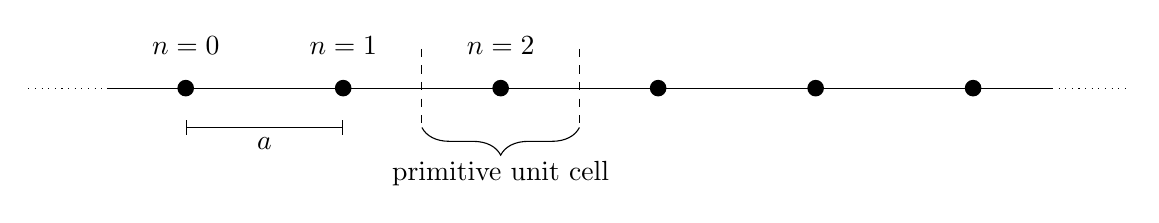
\begin{tikzpicture}
	\draw[dotted] (0,0) -- (1,0);
	\fill (2,0) circle (3pt) node[above,yshift=0.3cm] {$n = 0$};
	\fill (4,0) circle (3pt) node[above,yshift=0.3cm] {$n = 1$};
	\fill (6,0) circle (3pt) node[above,yshift=0.3cm] {$n = 2$};
	\fill (8,0) circle (3pt);
	\fill (10,0) circle (3pt);
	\fill (12,0) circle (3pt);
	\draw (1,0) -- (13,0);
	\draw[dotted] (13,0) -- (14,0);
	\draw[|-|] (2,-0.5) --node[below] {$a$} (4,-0.5);
	\draw[dashed] (5,0.5) -- (5,-0.5);
	\draw[dashed] (7,0.5) -- (7,-0.5);
	\draw[decorate,decoration={brace,amplitude=10pt,mirror}] (5,-0.5) -- (7,-0.5) node[below,midway,yshift=-0.3cm] {primitive unit cell};
\end{tikzpicture}\\
where $a$ is the lattice constant. Different atoms will be labeled by the integer index $n$. The crystal can be created by translating the primitive unit cell by the lattice constant. The location of the $n^{\trm{th}}$ atom is $na$.\\

Every atom has a single valence electron. Let $\ket{n}$ represent the electron localized at the $n^{\trm{th}}$ atom. Quantum mechanically, one expects the motion of electrons to occur due to tunneling through the chain. Say the energy of the electron $\ket{n}$ localized to an atom is $\bra{n}H\ket{n}=\varepsilon_{0}=0$. Let the probability amplitude for tunneling be $t$. Thus
\begin{equation}
\bra{n\pm1}H\ket{n}=-t
\end{equation} 

Therefore
\begin{equation}
H=-t\sum_{n}(\ketbra{n+1}{n}+\ketbra{n-1}{n})
\end{equation}
Note that no diagonal terms exist since $\varepsilon_{0}=0$.\\

\vspace{0.5cm}
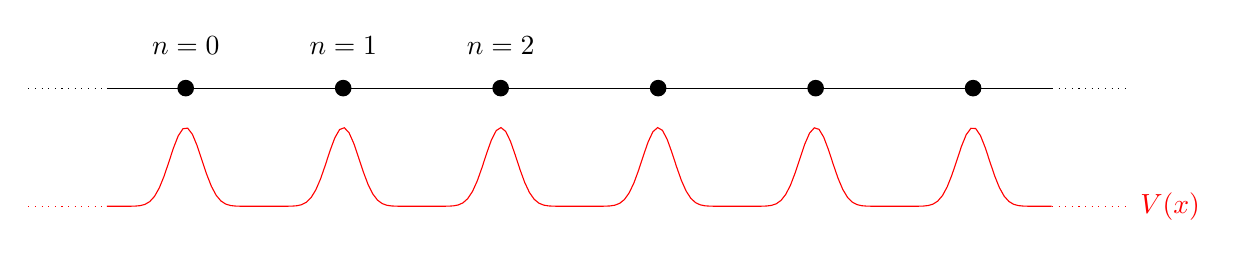
\begin{tikzpicture}
	\draw[dotted] (0,0) -- (1,0);
	\fill (2,0) circle (3pt) node[above,yshift=0.3cm] {$n = 0$};
	\fill (4,0) circle (3pt) node[above,yshift=0.3cm] {$n = 1$};
	\fill (6,0) circle (3pt) node[above,yshift=0.3cm] {$n = 2$};
	\fill (8,0) circle (3pt);
	\fill (10,0) circle (3pt);
	\fill (12,0) circle (3pt);
	\draw[dotted] (13,0) -- (14,0);
	\draw (1,0) -- (13,0);
	\draw[dotted,red] (0,-1.5) -- (1,-1.5); 
	\draw[domain=1:13,samples=200,red] plot (\x, {(cos(deg(pi/2*(\x-2))))^10 - 1.5});
	\draw[dotted,red] (13,-1.5) -- (14,-1.5) node[right] {$V(x)$};
\end{tikzpicture}
\vspace{0.5cm}

From the Heisenberg uncertainty principle: $\Delta p \Delta x \sim \hbar$. Therefore
\begin{equation}
E_\trm{min}\sim\frac{\Delta p^{2}}{2m}\sim\frac{\hbar^{2}}{2m\Delta x^{2}}
\end{equation}

When $t$ is positive, $t$ describes the energy gain due to localization of an electron between neighbouring atoms.\\

Let us find the eigenstates of $H$. Since $H$ is non-diagonal in the $\ket{n}$ basis, let us use the \ul{lattice Fourier transform} to obtain H in a different basis. The lattice Fourier transform is given by
\begin{equation}\label{eq:4}
\ket{n}=\sum_{k}\ket{k}\braket{k}{n}
\end{equation}
where $k$ is a wavevector of the electron and $p=\hbar k$ is its momentum.\\

For free electrons, we know that $\braket{x}{k}\sim e^{ikx}$. Thus, analogously $\braket{n}{k}\sim e^{ikna}$. Thus far, no restrictions have been placed on the range of $n$. Since a real substance will posses a finite number of unit cells, let us say that there are $N$ unit cells, such that $n$ runs from 0 to $N-1$. Since $\abs{\braket{n}{k}}^{2}$ is the probability an electron is found localized to atom $n$, $\sum_{n}\abs{\braket{n}{k}}^{2}=1$. Let the normalization constant be $C$.
\begin{equation}\label{eq:5}
\begin{aligned}
1&=\sum_{n=0}^{N-1}\abs{\braket{n}{k}}^{2}\\
&=\sum_{n=0}^{N-1}\abs{Ce^{ikna}}^{2}\\
&=NC^{2}\\
\implies C &= \frac{1}{\sqrt{N}}
\end{aligned}
\end{equation}

Thus, from equations \eqref{eq:4} and \eqref{eq:5}
\begin{equation}\label{eq:6}
\begin{aligned}
\braket{n}{k}&=\frac{1}{\sqrt{N}}e^{ikna}\\
\implies \ket{n}&=\frac{1}{\sqrt{N}}\sum_{k}e^{-ikna}\ket{k}
\end{aligned}
\end{equation}

What do we do at the boundaries of finite sized lattices? One could apply periodic boundary conditions. This allows us to avoid talking about boundaries when $N$ is large.\\
\begin{center}
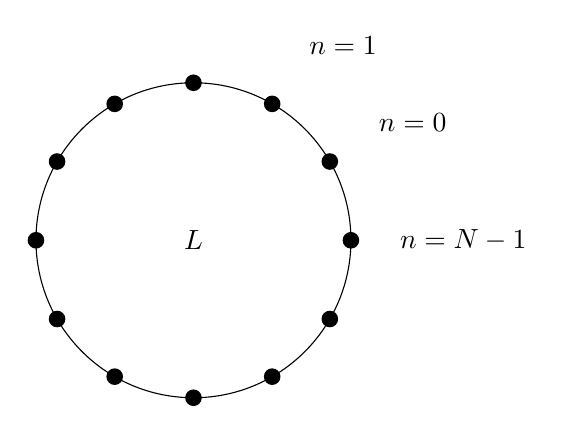
\begin{tikzpicture}
	\draw circle (2cm) node {$L$};
	\foreach \a in {3,4,...,11}{
		\fill (\a*360/12: 2cm) circle (3pt);
	}
	\fill (360/12: 2cm) circle (3pt) node[right,yshift=0.5cm,xshift=0.5cm] {$n=0$};
	\fill (2*360/12: 2cm) circle (3pt) node[above,yshift=0.5cm,xshift=0.9cm] {$n=1$};
	\fill (360: 2cm) circle (3pt) node[right,xshift=0.5cm] {$n=N-1$};
\end{tikzpicture}
\end{center}
This allows us to better consider the electrons if we are concerned only with the bulk properties of the system. Thus
\begin{equation}\label{eq:7}
\ket{n}=\ket{n+N}
\end{equation}
Therefore, from equations \eqref{eq:6} and \eqref{eq:7}
\begin{equation}
\begin{aligned}
\braket{n+N}{k}&=\braket{n}{k}\\
\implies e^{ik(n+N)a}&=e^{ikna}\\
\implies e^{ikNa}&=1
\end{aligned}
\end{equation}
Finally, this leads to
\begin{equation}
k=\frac{2\pi m}{Na}=\frac{2\pi m}{L}, m \in \mathbb{Z}
\end{equation}
Thus, values of $k$ are discrete, justifying writing $\ket{n}$ as a sum over $k$ rather than as an integral. This allows us to write the Hamiltonian as
\begin{equation}
H=-\frac{t}{N}\sum_{n=0}^{N-1}\sum_{k_{1}k_{2}}(\ketbra{k_{1}}{k_{2}}e^{-ik_{1}(n+1)a}e^{ik_{2}na}+\ketbra{k_{1}}{k_{2}}e^{-ik_{1}(n-1)a}e^{ik_{2}na})
\end{equation}

Note that
\begin{equation}
\frac{1}{N}\sum_{k=1}^{N}e^{2\pi i\frac{k}{N}(n-m)}=\delta_{nm}
\end{equation}
Since $k_{1}-k_{2}$ is a multiple of $\frac{2\pi}{Na}$
\begin{equation}
\frac{1}{N}\sum_{n=0}^{N-1}e^{-i(k_{1}-k_{2})na}=\delta_{k_{1}k_{2}}
\end{equation}
Thus, one writes
\begin{equation}
\begin{aligned}
H&=-t\sum_{k}\ketbra{k}{k}(e^{-ika}+e^{ika})\\
&=-2t\sum_{k}\cos(ka)\ketbra{k}{k}\\
&=\sum_{k}\varepsilon(k)\ketbra{k}
\end{aligned}
\end{equation}

Thus, the energy eigenvalues (energy level of state) $\varepsilon(k)$ are $-2t\cos(ka)$ for an electron moving in a 1D periodic potential. Contrast this with $\varepsilon(k)$ for a free electron, where
\begin{equation}
\varepsilon(k)=\frac{p^{2}}{2m}=\frac{\hbar^{2}k^{2}}{2m}
\end{equation}

$t$ acts as a tunneling coefficient that dictates a tunneling rate (up to a constant $\hbar$). The eigenstates $\ket{k}$ are
\begin{equation}
\ket{k}=\sum_{n}\ket{n}\braket{n}{k}=\frac{1}{\sqrt{N}}\sum_{n}\ket{n}e^{ikna}
\end{equation}
The kets $\ket{k}$ are called \ul{Bloch states}.\\

Suppose one transforms $k$ into $k+\frac{2\pi m}{a}, m\in\mathbb{Z}$. The Bloch state does not change
\begin{equation}
\begin{aligned}
\ket{k+\frac{2\pi m}{a}}&=\frac{1}{\sqrt{N}}\sum_{n}e^{i\left(k+\frac{2\pi m}{a}\right)na}\ket{n}\\
&=\frac{1}{\sqrt{N}}e^{ikna}\cancelto{1}{e^{i2\pi mn}}\ket{n}\\
&=\ket{k}
\end{aligned}
\end{equation}
Note that this is not dependent on the periodic boundary condition. Thus, physically distinct values of $k$ are restricted to a finite interval in $k$-space of length $\frac{2\pi}{a}$. Taking this to be symmetric around $k=0$
\[
-\frac{\pi}{a}\leq k < \frac{\pi}{a}\quad\trm{(\ul{First Brillouin zone})}
\]

\hspace{-1cm}
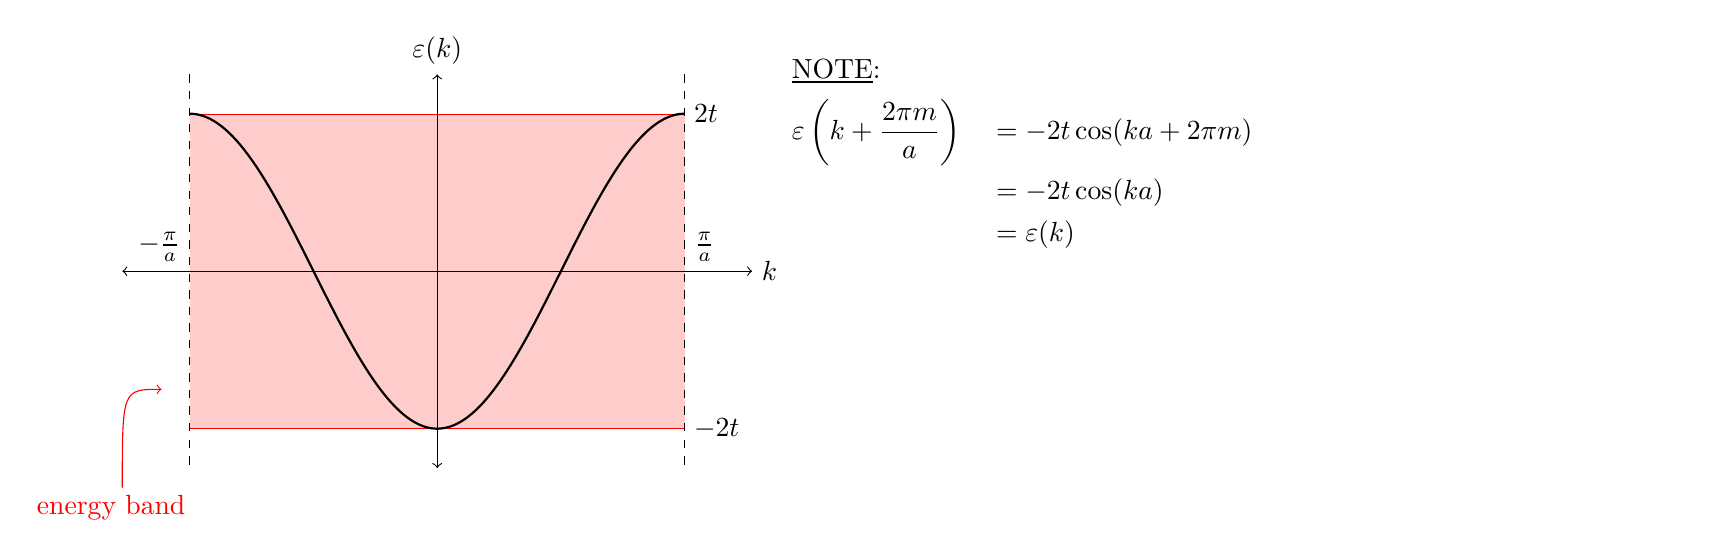
\begin{tikzpicture}
	\fill[red, fill opacity=0.2, text opacity=1] (pi,2) rectangle (-pi,-2) node[xshift=-1cm,yshift=-1cm] {energy band};
	\draw[line width=0.05mm, red, text=black] (-pi,2) -- (pi,2) node[right] {$2t$};
	\draw[line width=0.05mm, red, text=black] (-pi,-2) -- (pi,-2) node[right] {$-2t$};
	\draw[red,->] (-4,-2.75) .. controls (-4,-1.5) .. (-3.5,-1.5);
	\draw[<->] (-4,0) -- (4,0) node[right] {$k$};
	\draw[<->] (0,-2.5) -- (0,2.5) node[above] {$\varepsilon(k)$};
	\draw[thick,domain=-pi:pi,samples=200] plot (\x, {-2*cos(deg(\x)});
	\draw[dashed] (-pi,2.5) -- node[above left] {$-\frac{\pi}{a}$} (-pi,-2.5); 
	\draw[dashed] (pi,2.5) -- node[above right] {$\frac{\pi}{a}$} (pi,-2.5);
	\node[anchor=north west,right] at (3.5,1.5)
		{\[
			\begin{aligned}
				&\trm{\ul{NOTE}:}\\
				&\varepsilon\left(k+\frac{2\pi m}{a}\right)&&=-2t\cos(ka+2\pi m)\\
				& &&=-2t\cos(ka)\\
				& &&=\varepsilon(k)
			\end{aligned}
		\]};
\end{tikzpicture}\\
The accessible energy levels are confined to the finite interval between $\varepsilon_{\trm{max}}=2t$ and $\varepsilon_{\trm{min}}=-2t$. It has a \ul{bandwidth} $\Delta\varepsilon=\varepsilon_{\trm{max}}-\varepsilon_{\trm{min}}=4t$. The interval of allowed values of energy is called an \ul{energy band}.

\begin{align*}
\trm{\ul{Aside}:}\quad\ket{k}&=\frac{1}{\sqrt{N}}\sum_{n}e^{ikna}\ket{n}\trm{ is the \ul{lattice Fourier transform}}.\\
\ket{n}&=\frac{1}{\sqrt{N}}\sum_{k}e^{-ikna}\ket{k}\trm{ is the \ul{inverse lattice Fourier transform}}.
\end{align*}

In general, the energy spectrum of electrons in a solid takes the form of several bands separated by \ul{band gaps} (intervals of forbidden values).\\

How many quantum states are there in a band? Due to periodic boundary conditions
\begin{equation}
\begin{aligned}
-\frac{\pi}{a}&\leq k<\frac{\pi}{a}\\
-\frac{\pi}{a}&\leq\frac{2\pi m}{Na}<\frac{\pi}{a}\\
-\frac{N}{2}&\leq m<\frac{N}{2}
\end{aligned}
\end{equation}

Since $m$ is an integer, there are $N$ allowed values for $m$ (and hence $k$). Accounting for the spins of electrons, there are actually $2N$ states available in every band. Suppose one has one valence electron for each of the $N$ atoms in the chain. Thus, there will be $N$ electrons. By Pauli's exclusion principle, which states that only one fermion can occupy a given state in a band, exactly half of the total number of states in the band will be filled.
\begin{center}
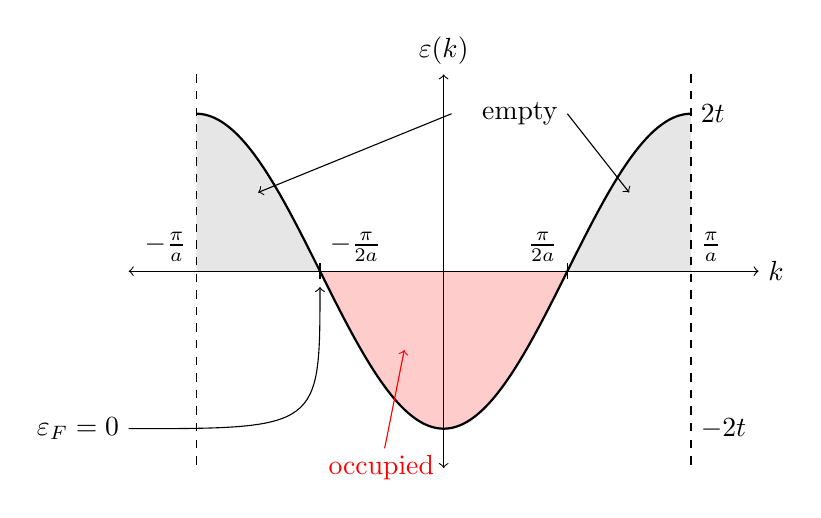
\begin{tikzpicture}
	\fill [gray,domain=-pi:-pi/2,fill opacity=0.2] (-pi,0) -- plot (\x, {-2*cos(deg(\x)}) -- (-pi/2,0) -- cycle;
	\fill [red,domain=-pi/2:pi/2,fill opacity=0.2] (-pi/2,0) -- plot (\x, {-2*cos(deg(\x)}) -- (pi/2,0) -- cycle;
	\fill [gray,domain=pi/2:pi,fill opacity=0.2] (pi/2,0) -- plot (\x, {-2*cos(deg(\x)}) -- (pi,0) -- cycle;
	\draw[<->] (-4,0) -- (4,0) node[right] {$k$};
	\draw[<->] (0,-2.5) -- (0,2.5) node[above] {$\varepsilon(k)$};
	\draw[thick,domain=-pi:pi,samples=200] plot (\x, {-2*cos(deg(\x)});
	\draw[dashed] (-pi,2.5) -- node[above left] {$-\frac{\pi}{a}$} (-pi,-2.5); 
	\draw[dashed] (pi,2.5) -- node[above right] {$\frac{\pi}{a}$} (pi,-2.5);
	\draw (pi,2) node[right] {$2t$};
	\draw (pi,-2) node[right] {$-2t$};
	\draw (pi/2,0.1) --node[above left] {$\frac{\pi}{2a}$} (pi/2,-0.1);
	\draw (-pi/2,0.1) --node[above right] {$-\frac{\pi}{2a}$} (-pi/2,-0.1);
	\draw[red] (0,-2.5) node[left] {occupied};
	\draw[red,->] (-0.75,-2.25) -- (-0.5,-1);
	\draw (pi/2,2) node[left] {empty};
	\draw[->] (pi/2,2) -- (3*pi/4,1);
	\draw[->] (0.1,2) -- (-3*pi/4,1);
	\draw[->] (-4,-2) node[left] {$\varepsilon_{F}=0$} .. controls(-pi/2,-2) .. (-pi/2,-0.2);
\end{tikzpicture}
\end{center}
When the electrons in the material are at zero temperature, the electrons occupy all of the lowest possible energy states. The \ul{Fermi energy} ($\varepsilon_{F}$) for a system occurs at the interface between filled energy states and unfilled energy states at zero temperature for non-interacting fermions. Thus, $\varepsilon_{F}=0$ in this problem.\\

Note that in this problem, any perturbation will excite an electron below $\varepsilon_{F}$ to above $\varepsilon_{F}$. An infinitesimally small electric field can achieve this, which is a property of metals. In fact, if the Fermi energy crosses a band, it is a metal.\bigskip

To find the corresponding $k$ for $\varepsilon_{F}=0$
\begin{equation}
\varepsilon(k)=\varepsilon_{F}=0\quad\implies\quad k=\pm\frac{\pi}{2a}=\pm k_{F}
\end{equation}
where $k_{F}$ is the \ul{Fermi wave vector}. Again, $k_{F}$ separates filled states from empty states. $\abs{k}<k_{F}$ are filled states while $\abs{k}>k_{F}$ are empty states. The surface in momentum space (or $k$-space) separating filled and unfilled states is the \ul{Fermi surface}. Most observed properties of a metal follow from the existence of the Fermi surface. The dimension of the Fermi surface is one less than the dimension of the system.\\

The volume of filled states in $k$-space bounded by the Fermi surface (or the volume of the Fermi sea) is related to the density of electrons

\begin{equation}
	\tikzmarknode{A}{2}\left[\frac{\tikzmarknode{B}{(2k_{F})}}{\tikzmarknode{C}{\left(\frac{2\pi}{Na}\right)}}\right]=\tikzmarknode{D}{n}\tikzmarknode{E}{(Na)}
\end{equation}
\begin{tikzpicture}[overlay,remember picture,shorten <=1mm,font=\footnotesize]
	\draw[red,<-] (A.south) -- ++ (-0.3,-0.3) node[left,xshift=0.1cm,yshift=-0.1cm] {2 spin states};
	\draw[red,<-] (B.east) -- ++ (1,0.6) node[right] {volume of Fermi sea};
	\draw[red,<-] (C.south) -- ++ (0.2,-0.4) node[below right,xshift=-0.1cm,yshift=0.2cm] {volume corresponding to a single $k$ since $k$ is quantized as $k=\frac{2\pi m}{Na}$, $m\in\mathbb{Z}$};
	\draw[red,<-] (D.south) -- ++ (0.3,-0.3) node[right,xshift=-0.1cm,yshift=-0.1cm] {number density};
	\draw[red,<-] (E.east) -- ++(0.8,0.2) node[right] {length of chain};
\end{tikzpicture}

Thus
\begin{equation}
k_{F}=\frac{\pi}{2}n
\end{equation}

This makes sense as that implies $n=\frac{1}{a}$ which is true as there is one electron per unit cell. In fact, this result is always true and arises from \ul{Luttinger's theorem}, which states that the volume enclosed by the Fermi surface is directly propertional to the electron density.

\subsection{Polyacetylene}
This model can be modified to represent the one-dimensional crystalline polymer polyacetylene. It consists of weakly-interacting 1D chains of CH units.  The electronic configuration of H and C are given by $1s$ and $1s^{2}2s^{2}2p^{2}$ respectively.

\begin{figure}[H]
	\centering
	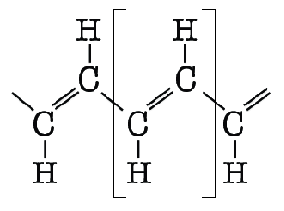
\includegraphics{Images/2/polyacetylene.png}
	\caption{Polyacetylene with unit cell}
\end{figure}
H has one valence electron while C has four valence electrons. Two of these electrons are used to covalently bond with nearest-neighbour carbon atoms. The third electron is used to bond with its corresponding hydrogen neighbour All other electrons in the inner orbitals are tightly bound to the carbon nuclei. Thus, one valence electron is free to move along the chain per carbon atom.\bigskip

If all the bonds between the carbons were the same, we would obtain our previous model. However, due to \ul{Peierl's instability}, adjacent CH groups move toward each other. This leads to alternating single and double bonds. Note that the carbons of a double bond are closer together than those of a single bond. This can be represented in the following model\\
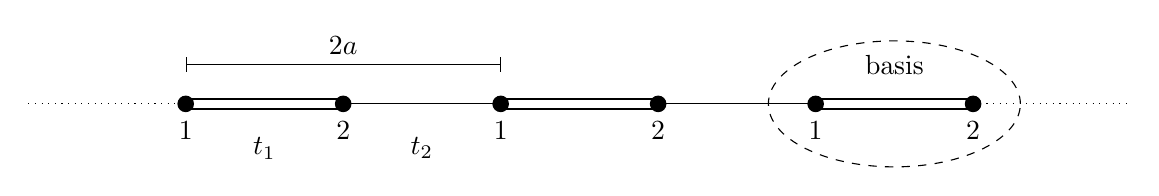
\begin{tikzpicture}
	\draw[double=none,double distance=3pt,thick] (2,0) -- node[below,yshift=-0.3cm] {$t_{1}$} (4,0);
	\draw[double=none,double distance=3pt,thick] (6,0) -- (8,0);
	\draw[double=none,double distance=3pt,thick] (10,0) -- (12,0);
	\draw[dotted] (0,0) -- (2,0);
	\fill (2,0) circle (3pt) node[below,yshift=-0.1cm] {$1$};
	\fill (4,0) circle (3pt) node[below,yshift=-0.1cm] {$2$};
	\fill (6,0) circle (3pt) node[below,yshift=-0.1cm] {$1$};
	\fill (8,0) circle (3pt) node[below,yshift=-0.1cm] {$2$};
	\fill (10,0) circle (3pt) node[below,yshift=-0.1cm] {$1$};
	\fill (12,0) circle (3pt) node[below,yshift=-0.1cm] {$2$};
	\draw[dotted] (12,0) -- (14,0);
	\draw (4,0) -- node[below,yshift=-0.3cm] {$t_{2}$} (6,0);
	\draw (8,0) -- (10,0);
	\draw[|-|] (2,0.5) -- node[above] {$2a$} (6,0.5);
	\draw[dashed] (11,0) circle[x radius=1.6cm,y radius=0.8cm] node[yshift=0.5cm] {basis};
\end{tikzpicture}\\
The primitive unit cell has now doubled in size and now contains atoms 1 and 2. As an aside, the number of bands in a solid is equal to the number of atoms in the basis of a primitive unit cell.\\

The double and single bonds have different tunneling amplitudes, namely $t_{1}$ and $t_{2}$ respectively, with $t_{1}>t_{2}$. The lattice points of this model are collectively known as the \ul{Bravais lattice}. However, in this case, the Bravais lattice points are associated with two physical atoms composing the \ul{basis}. One can describe any \ul{crystal} with a basis and a Bravais lattice.\\

Let $\ket{n,\alpha}$, $\alpha\in\{1,2\}$ describe the electron localized to the $n^{\trm{th}}$ unit cell at atom $\alpha$. The Hamiltonian characterizing the possible transitions is described by
\begin{equation}\label{eq:19}
H=\sum_{n}\bigg[-t_{1}\big(\ketbra{n,2}{n,1}+\ketbra{n,1}{n,2}\big)-t_{2}\big(\ketbra{n-1,2}{n,1}+\ketbra{n,1}{n-1,2}\big)\bigg]
\end{equation}
Note in this case, $n$ labels the unit cell. This recurring motif of tunneling only to the nearest-neighbour atoms is known as the \ul{tight-binding model}.\\

As before, let us transform $\ket{n,\alpha}$ into momentum space
\begin{equation}
\ket{n,\alpha}=\sum_{k}\ket{k,\alpha}\braket{k,\alpha}{n,\alpha}
\end{equation}
Again, $\braket{x,k}\sim e^{ikx}$. Thus, by analogy $\braket{n,\alpha}{k,\alpha}\sim e^{2ikna}$. Using the same argument as before, the normalization constant is $C=\frac{1}{\sqrt{N}}$ Note that $N$ is the number of unit cells and not simply the number of atoms. Thus
\begin{equation}
\ket{n,\alpha}=\frac{1}{\sqrt{N}}\sum_{k}e^{-2ikna}\ket{k,\alpha}
\end{equation}

Using the periodic boundary conditions $\ket{n,\alpha}=\ket{n+N,\alpha}$, one obtains $e^{2ikna}=1$. Thus, $k$ is quantized as
\begin{equation}
k=\frac{\pi m}{Na}, m\in\mathbb{Z}
\end{equation}
If one transforms $k$ into $k+\frac{\pi m}{a}$, $m\in\mathbb{Z}$, one sees again that the Bloch states do not change. This implies the physically distanct values of $k$ are restricted to a finite interval of $\frac{\pi}{a}$ in $k$-space. Taken symmetrically around $k=0$
\begin{equation}
-\frac{\pi}{2a}\leq k<\frac{\pi}{2a}
\end{equation}
The Brillouin zone for polyacetylene is half the width of the Brillouin zone for the original toy model, since the unit cell is now twice the size.\\

Since the deviation between tunneling amplitudes is slight, let $2\delta t=t_{1}-t_{2}$ be a small perturbation such that
\begin{equation}
t_{1}=t+\delta t, \quad t_{2}=t-\delta t
\end{equation}

Therefore, substituting into equation \eqref{eq:19}
\begin{equation}
\begin{aligned}
H=&-(t+\delta t)\frac{1}{N}\sum_{n}\sum_{k_{1}k_{2}}\big(\ketbra{k_{1},2}{k_{2},1}e^{-2ik_{1}na}e^{2ik_{2}na}+\ketbra{k_{1},1}{k_{2},2}e^{-2ik_{1}na}e^{2ik_{2}na}\big)\\
&-(t-\delta t)\frac{1}{N}\sum_{n}\sum_{k_{1}k_{2}}\big(\ketbra{k_{1},2}{k_{2},1}e^{-2ik_{1}(n-1)a}e^{2ik_{2}na}+\ketbra{k_{1},1}{k_{2},2}e^{-2ik_{1}na}e^{2ik_{2}(n-1)a}\big)\\
=&-(t+\delta t)\sum_{k}\big(\ketbra{k,1}{k,2}+\ketbra{k,2}{k,1}\big)-(t-\delta t)\sum_{k}\big(\ketbra{k,1}{k,2}e^{-2ika}+\ketbra{k,2}{k,1}e^{2ika}\big)\\
&\explain\trm{ Since } \frac{1}{N}\sum_{n}e^{-2i(k-k')na}=\delta_{kk'}\\
=&-t\sum_{k}(1+e^{-2ika})\ketbra{k,1}{k,2}-\delta t\sum_{k}(1-e^{-2ika})\ketbra{k,1}{k,2}\\
&-t\sum_{k}(1+e^{2ika})\ketbra{k,2}{k,1}-\delta t\sum_{k}(1-e^{2ika})\ketbra{k,2}{k,1}
\end{aligned}
\end{equation}

At fixed $k$, this resembles the Hamiltonian of a spin in a magnetic field
\begin{equation}
H(k)=-t(1+e^{-2ika})\ketbra{1}{2}-\delta t(1-e^{-2ika})\ketbra{1}{2}+\trm{h.c.}
\end{equation}
where
\begin{equation}
H=\sum_{k}H(k)
\end{equation}\\

Here we denote $\ket{k,1}$ as $\ket{1}$ and $\ket{k,2}$ as $\ket{2}$. Recall from quantum mechanics that for a spin in a magnetic field
\begin{equation}
H=\vec{B}\cdot\vec{S}=\frac{\hbar}{2}\vec{B}\cdot\vec{\sigma}
\end{equation}
where $\vec{\sigma}=\{\sigma_{x},\sigma_{y},\sigma_{z}\}$ are the \ul{Pauli matrices}.
\begin{equation}
\begin{aligned}
\sigma_{x}&=\ketbra{\up}{\dn}+\ketbra{\dn}{\up}=\ketbra{1}{2}+\ketbra{2}{1}\\
&=\begin{bmatrix}
0 & 1\\
1 & 0
\end{bmatrix}\\
\sigma_{y}&=-i(\ketbra{\up}{\dn}-\ketbra{\dn}{\up})=-i(\ketbra{1}{2}-\ketbra{2}{1})\\
&=\begin{bmatrix}
0 & -i\\
i & 0
\end{bmatrix}\\
\sigma_{z}&=\ketbra{\up}{\up}-\ketbra{\dn}{\dn}=\ketbra{1}{1}-\ketbra{2}{2}\\
&=\begin{bmatrix}
1 & 0\\
0 & -1
\end{bmatrix}
\end{aligned}
\end{equation}

In terms of sinusoidal functions ($e^{2ika}=\cos(2ka)+i\sin(2ka)$)
\begin{equation}
\begin{aligned}
H(k)=&-\big[(t+\delta t)+(t-\delta t)\cos(2ka)\big]\ketbra{1}{2}\\
&\quad+i(t-\delta t)\sin(2ka)\ketbra{1}{2}\\
&\quad-\big[(t+\delta t)+(t-\delta t)\cos(2ka)\big]\ketbra{2}{1}\\
&\quad-i(t-\delta t)\sin(2ka)\ketbra{2}{1}
\end{aligned}
\end{equation}

Let us introduce $\vec{d}(k)=\{d_{x}(k),d_{y}(k),d_{z}(k)\}$, such that
\begin{equation}
\begin{aligned}
d_{x}(k)&=-(t+\delta t)-(t-\delta t)\cos(2ka)\\
d_{y}(k)&=-(t-\delta t)\sin(2ka)\\
d_{z}(k)&=0
\end{aligned}
\end{equation}

Thus
\begin{equation}
H(k)=\vec{d}(k)\cdot\vec{\sigma}=\begin{bmatrix}
0 & d_{x}-id_{y}\\
d_{x}+id_{y} & 0
\end{bmatrix}
\end{equation}

As has been found previously in quantum mechanics (PHYS 434), the eigenvalues $\varepsilon(k)$ of $H(k)$ correspond to spin $\vec{\sigma}$ aligning or anti-aligning to $\vec{d}(k)$.
\begin{equation}
\begin{aligned}
0=\det(H(k)-\varepsilon\mathbb{I})=\varepsilon^{2}-(d_{x}^{2}+d_{y}^{2})\\
\implies\varepsilon(k)=\pm\sqrt{d_{x}^{2}(k)+d_{y}^{2}(k)}=\pm\abs*{\vec{d}(k)}
\end{aligned}
\end{equation}

\aside{The spin correspondence $\ket{1}=\ket{\up}$ and $\ket{2}=\ket{\dn}$ is referred to as a \ul{pseudospin}. $\vec{d}(k)$ is an \ul{effective magnetic field}.}

Note that in contrast to the single energy band in the previous model, there are now two energy bands, since there are two valence orbitals per unit cell. In general, each distinct state (atom) in the unit cell gives rise to a band.
\begin{equation}
\begin{aligned}
\abs*{\vec{d}(k)}^{2}&=d_{x}^{2}(k)+d_{y}^{2}(k)+d_{z}^{2}(k)\\
&=\big[-(t+\delta t)-(t-\delta t)\cos(2ka)\big]^{2}+\big[-(t-\delta t)\sin(2ka)\big]^{2}+0^{2}\\
&=(t+\delta t)^{2}+2(t^{2}-\delta t^{2})\cos(2ka)+(t-\delta t)^{2}\cos^{2}(2ka)+(t-\delta t)^{2}\sin^{2}(2ka)\\
&=t^{2}+2t\delta t+\delta t^{2}+2(t^{2}-\delta t^{2})\cos(2ka)+t^{2}-2t\delta t+\delta t^{2}\\
&=2t^{2}\big(1+\cos(2ka)\big)+2\delta t^{2}\big(1-\cos(2ka)\big)\\
&=2t^{2}\big(2\cos^{2}(ka)\big)+2\delta t^{2}\big(2\sin^{2}(ka)\big)\\
&=4t^{2}\cos^{2}(ka)+4\delta t^{2}\sin^{2}(ka)\\
\end{aligned}
\end{equation}

Thus
\begin{equation}
\varepsilon(k)=\pm\abs*{\vec{d}(k)}=\pm\sqrt{4t^{2}\cos^{2}(ka)+4\delta t^{2}\sin^{2}(ka)}
\end{equation}

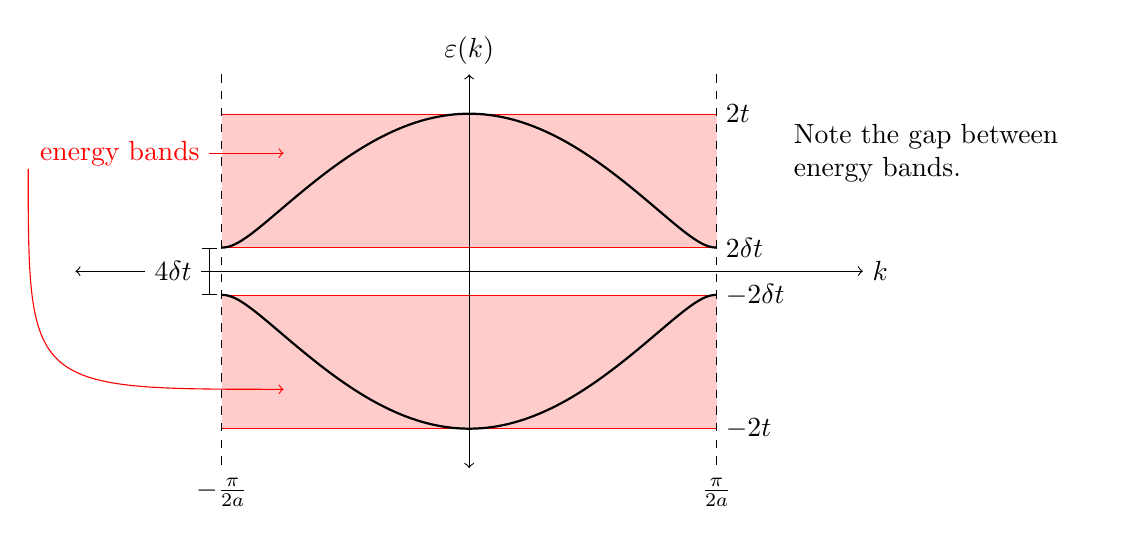
\begin{tikzpicture}
	\fill[red, fill opacity=0.2, text opacity=1] (pi,2) rectangle (-pi,0.3);
	\fill[red, fill opacity=0.2, text opacity=1] (pi,-2) rectangle (-pi,-0.3);
	\draw[line width=0.05mm, red, text=black] (-pi,2) -- (pi,2) node[right] {$2t$};
	\draw[line width=0.05mm, red, text=black] (-pi,-2) -- (pi,-2) node[right] {$-2t$};
	\draw[line width=0.05mm, red, text=black] (-pi,0.3) -- (pi,0.3) node[right] {$2\delta t$};
	\draw[line width=0.05mm, red, text=black] (-pi,-0.3) -- (pi,-0.3) node[right] {$-2\delta t$};
	\draw[<->] (-5,0) -- (5,0) node[right] {$k$};
	\draw[<->] (0,-2.5) -- (0,2.5) node[above] {$\varepsilon(k)$};
	\draw[thick,domain=-pi:pi,samples=200] plot (\x, {sqrt(4*cos(deg(\x/2))^2+0.09*sin(deg(\x/2))^2});
	\draw[thick,domain=-pi:pi,samples=200] plot (\x, {-sqrt(4*cos(deg(\x/2))^2+0.09*sin(deg(\x/2))^2});
	\draw[dashed] (-pi,2.5) -- (-pi,-2.5) node[below] {$-\frac{\pi}{2a}$}; 
	\draw[dashed] (pi,2.5) -- (pi,-2.5) node[below] {$\frac{\pi}{2a}$};
	\draw[|-|] (-3.3,0.3) --node[left,fill=white,xshift=-0.1cm] {$4\delta t$} (-3.3,-0.3);
	\draw[red] (-3.3,1.5) node[left] {energy bands};
	\draw[red,->] (-3.3,1.5) -- (-3*pi/4,1.5);
	\draw[red,->] (-5.6,1.3) .. controls(-5.6,-1.5) .. (-3*pi/4,-1.5);
	\node[anchor=north west,right,text width=4cm] at (4,1.5)
		{Note the gap between energy bands.};
\end{tikzpicture}

As we increased the size of our unit cell from $a$ to $2a$, the Brillouin zone went from $k\in\left[-\frac{\pi}{a},\frac{\pi}{a}\right)$ to $k\in\left[-\frac{\pi}{2a},\frac{\pi}{2a}\right)$. In this model, since there is one free valence electron per carbon, there are two free valence electrons per unit cell. Recall that in the previous model, there were $2N$ states available in the band. Following the same arguments, the Brillouin zone decreases by a factor of 2 in this model. However, the amount between successive discrete values of $k$ also decreases by the same amount. Thus, there are still $2N$ states available per band. For $N$ unit cells, there are $2N$ electrons. By Pauli exclusion principle, the lowere band is completely filled, leaving the upper band empty. Since an energy of at least $4\delta t$ is required for an electron to transition across the Fermi surface, polyacetylene is an insulator (when $\delta t>0$).
\begin{center}
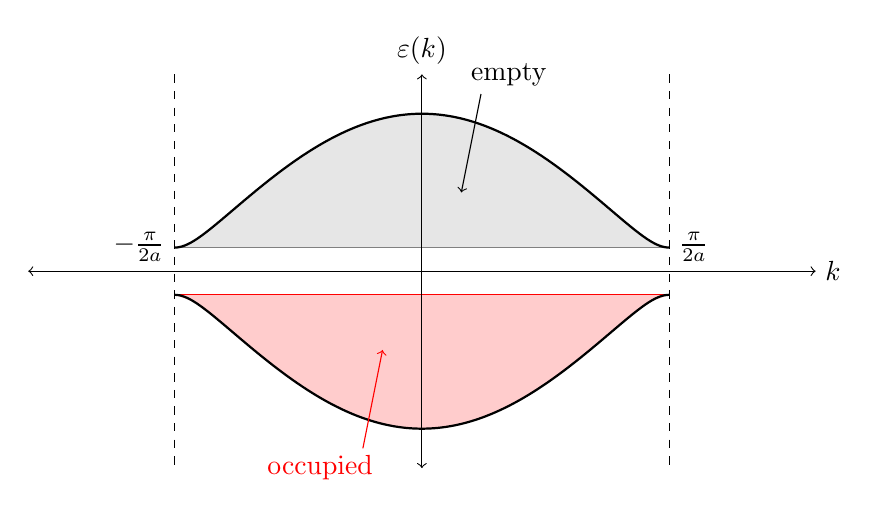
\begin{tikzpicture}
	\fill [gray,domain=-pi:pi,fill opacity=0.2] (-pi,0.3) -- plot (\x, {sqrt(4*cos(deg(\x/2))^2+0.09*sin(deg(\x/2))^2}) -- (pi,0.3) -- cycle;
	\fill [red,domain=-pi:pi,fill opacity=0.2] (-pi,-0.3) -- plot (\x, {-sqrt(4*cos(deg(\x/2))^2+0.09*sin(deg(\x/2))^2}) -- (pi,-0.3) -- cycle;
	\draw[gray] (-pi,0.3) -- (pi,0.3);
	\draw[red] (-pi,-0.3) -- (pi,-0.3);
	\draw[<->] (-5,0) -- (5,0) node[right] {$k$};
	\draw[<->] (0,-2.5) -- (0,2.5) node[above] {$\varepsilon(k)$};
	\draw[thick,domain=-pi:pi,samples=200] plot (\x, {sqrt(4*cos(deg(\x/2))^2+0.09*sin(deg(\x/2))^2});
	\draw[thick,domain=-pi:pi,samples=200] plot (\x, {-sqrt(4*cos(deg(\x/2))^2+0.09*sin(deg(\x/2))^2});
	\draw[dashed] (-pi,2.5) -- node[above left] {$-\frac{\pi}{2a}$} (-pi,-2.5) ; 
	\draw[dashed] (pi,2.5) -- node[above right] {$\frac{\pi}{2a}$} (pi,-2.5);
	\draw[red] (-0.5,-2.5) node[left] {occupied};
	\draw[red,->] (-0.75,-2.25) -- (-0.5,-1);
	\draw (0.5,2.5) node[right] {empty};
	\draw[->] (0.75,2.25) -- (0.5,1);
\end{tikzpicture}
\end{center}

Consider the limit when $\delta t\rightarrow0$. One should expect our first model, which is a metal.
\begin{equation}
\varepsilon(k)=\pm\sqrt{4t^{2}\cos^{2}(ka)}=\pm2t\cos(ka)
\end{equation}

\begin{center}
\begin{tikzpicture}
	\draw[<->] (-5,0) -- (5,0) node[right] {$k$};
	\draw[<->] (0,-2.5) -- (0,2.5) node[above] {$\varepsilon(k)$};
	\draw[thick,domain=-pi:pi,samples=200] plot (\x, {2*cos(deg(\x/2))});
	\draw[thick,domain=-pi:pi,samples=200] plot (\x, {-2*cos(deg(\x/2))});
	\draw[dashed] (-pi,2.5) -- node[above left] {$-\frac{\pi}{2a}$} (-pi,-2.5);
	\draw[dashed] (pi,2.5) -- node[above right] {$\frac{\pi}{2a}$} (pi,-2.5);
\end{tikzpicture}
\end{center}
This is simply the single band dispersion in the $-\frac{\pi}{a}$ to $\frac{\pi}{a}$ Brillouin zone folded into the halved $-\frac{\pi}{2a}$ to $\frac{\pi}{2a}$ Brillouin zone.\bigskip

Suppose the sign of $\delta t$ is flipped from $\delta t$ to $-\delta t$. Thus, one transitions from $t_{1}>t_{2}$ to $t_{2}>t_{1}$. Since a sign flip corresponds to the same pattern, but with a shift by $a$
\begin{center}
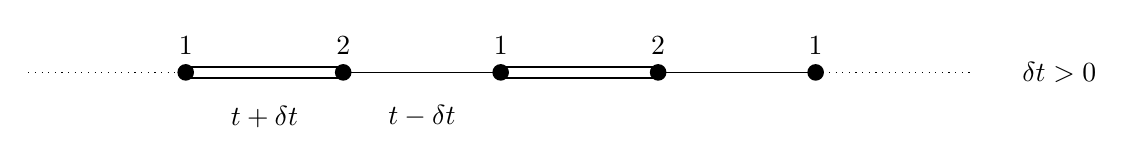
\begin{tikzpicture}
	\draw[double=none,double distance=3pt,thick] (2,0) -- node[below,yshift=-0.3cm] {$t+\delta t$} (4,0);
	\draw[double=none,double distance=3pt,thick] (6,0) -- (8,0);
	\draw[dotted] (0,0) -- (2,0);
	\fill (2,0) circle (3pt) node[above,yshift=0.1cm] {$1$};
	\fill (4,0) circle (3pt) node[above,yshift=0.1cm] {$2$};
	\fill (6,0) circle (3pt) node[above,yshift=0.1cm] {$1$};
	\fill (8,0) circle (3pt) node[above,yshift=0.1cm] {$2$};
	\fill (10,0) circle (3pt) node[above,yshift=0.1cm] {$1$};
	\draw[dotted] (10,0) -- (12,0) node[right,xshift=0.5cm] {$\delta t>0$};
	\draw (4,0) -- node[below,yshift=-0.3cm] {$t-\delta t$} (6,0);
	\draw (8,0) -- (10,0);
\end{tikzpicture}
\end{center}
\begin{center}
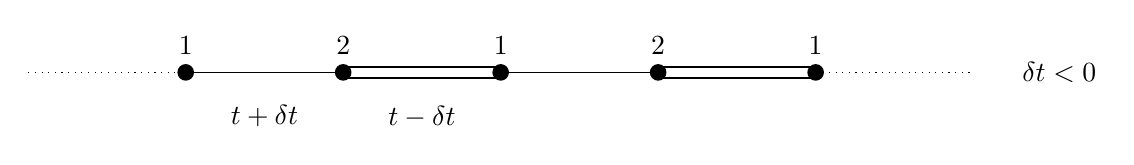
\begin{tikzpicture}
	\draw[double=none,double distance=3pt,thick] (4,0) -- node[below,yshift=-0.3cm] {$t-\delta t$} (6,0);
	\draw[double=none,double distance=3pt,thick] (8,0) -- (10,0);
	\draw[dotted] (0,0) -- (2,0);
	\fill (2,0) circle (3pt) node[above,yshift=0.1cm] {$1$};
	\fill (4,0) circle (3pt) node[above,yshift=0.1cm] {$2$};
	\fill (6,0) circle (3pt) node[above,yshift=0.1cm] {$1$};
	\fill (8,0) circle (3pt) node[above,yshift=0.1cm] {$2$};
	\fill (10,0) circle (3pt) node[above,yshift=0.1cm] {$1$};
	\draw[dotted] (10,0) -- (12,0) node[right,xshift=0.5cm] {$\delta t<0$};
	\draw (2,0) -- node[below,yshift=-0.3cm] {$t+\delta t$} (4,0);
	\draw (6,0) -- (8,0);
\end{tikzpicture}
\end{center}

This is a different state, although it has the same energy (degenerate) with the original state. Thus, polyacetylene has a doubly degenerate ground state. This degeneracy is related to the inversion symmetry with respect to any carbon atom. This degeneracy is spontaneously broken when one of the states is chosen.\\

The band dispersion depends only on $\delta t^{2}$ and does not change when $\delta t$ changes sign. However, $\vec{d}(k)$ is sensitive to the sign of $\delta t$. Let us see how $\vec{d}(k)$ changes as $k$ goes from $-\frac{\pi}{2a}$ to $\frac{\pi}{2a}$.
\[
\begin{aligned}
d_{x}\left(-\frac{\pi}{2a}\right)&=-2\delta t,\quad & d_{y}\left(-\frac{\pi}{2a}\right)&=0\\
d_{x}(0)&=-2t,\quad & d_{y}(0)&=0\\
\end{aligned}
\]

\begin{center}
\begin{tikzpicture}
	\draw[<->] (-2.5,0) -- (2.5,0) node[right] {$d_{x}$};
	\draw[<->] (0,-2.5) node[below] {$\delta t>0$} -- (0,2.5) node[above] {$d_{y}$};
	\draw (-1.15,0) circle[x radius=0.85cm,y radius=0.5cm];
\end{tikzpicture}\hfill
\begin{tikzpicture}
	\draw[<->] (-2.5,0) -- (2.5,0) node[right] {$d_{x}$};
	\draw[<->] (0,-2.5) node[below] {$\delta t<0$} -- (0,2.5) node[above] {$d_{y}$};
	\draw (-0.85,0) circle[x radius=1.15cm,y radius=0.5cm];
\end{tikzpicture}
\end{center}
Note that for $\delta t<0$, the origin is enclosed. Recall that $\varepsilon(k)=\pm\abs*{\vec{d}(k)}$. If $\abs*{\vec{d}(k)}\neq0$, there exists an energy gap between energy bands. Thus for $\delta t>0$, polyacetylene is a normal insulator, as found before. However, when $\delta t<0$, $\abs*{\vec{d}(k)}=0$ is enclosed, which leads us to refer to polyacetylene as a \ul{topological insulator} when $\delta t<0$. Effectively, there is no method to continuously deform the Hamiltonian (i.e. changing sign of $\delta t$) without merging the two energy bands. The transition from $\delta t>0$ to $\delta t<0$ permits the band gap to close temporarily.\\

\hspace{-1.1cm}
\mbox{
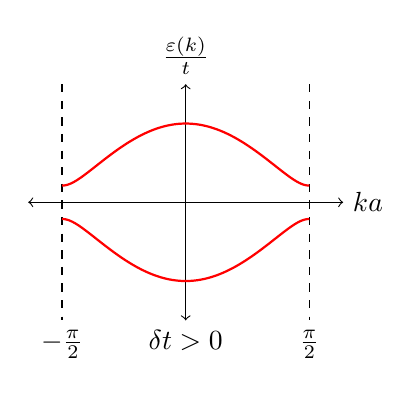
\begin{tikzpicture}[baseline=(current bounding box.center)]
	\draw[<->] (-2,0) -- (2,0) node[right] {$ka$};
	\draw[<->] (0,-1.5) node[below] {$\delta t>0$} -- (0,1.5) node[above] {$\frac{\varepsilon(k)}{t}$};
	\draw[dashed] (-pi/2,1.5) -- (-pi/2,-1.5) node[below] {$-\frac{\pi}{2}$};
	\draw[dashed] (pi/2,1.5) -- (pi/2,-1.5) node[below] {$\frac{\pi}{2}$};
	\draw[thick,domain=-pi/2:pi/2,samples=200,red] plot (\x, {sqrt(cos(deg(\x))^2+0.045*sin(deg(\x))^2});
	\draw[thick,domain=-pi/2:pi/2,samples=200,red] plot (\x, {-sqrt(cos(deg(\x))^2+0.045*sin(deg(\x))^2});
\end{tikzpicture}$\implies$
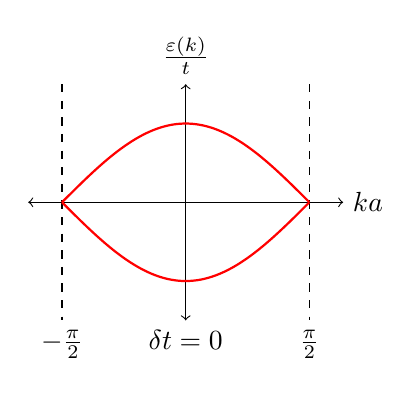
\begin{tikzpicture}[baseline=(current bounding box.center)]
	\draw[<->] (-2,0) -- (2,0) node[right] {$ka$};
	\draw[<->] (0,-1.5) node[below] {$\delta t=0$} -- (0,1.5) node[above] {$\frac{\varepsilon(k)}{t}$};
	\draw[dashed] (-pi/2,1.5) -- (-pi/2,-1.5) node[below] {$-\frac{\pi}{2}$};
	\draw[dashed] (pi/2,1.5) -- (pi/2,-1.5) node[below] {$\frac{\pi}{2}$};
	\draw[thick,domain=-pi/2:pi/2,samples=200,red] plot (\x, {cos(deg(\x))});
	\draw[thick,domain=-pi/2:pi/2,samples=200,red] plot (\x, {-cos(deg(\x))});
\end{tikzpicture}$\implies$
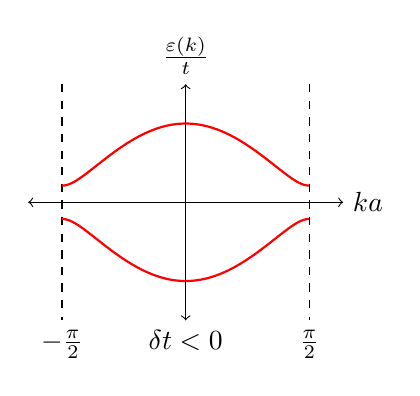
\begin{tikzpicture}[baseline=(current bounding box.center)]
	\draw[<->] (-2,0) -- (2,0) node[right] {$ka$};
	\draw[<->] (0,-1.5) node[below] {$\delta t<0$} -- (0,1.5) node[above] {$\frac{\varepsilon(k)}{t}$};
	\draw[dashed] (-pi/2,1.5) -- (-pi/2,-1.5) node[below] {$-\frac{\pi}{2}$};
	\draw[dashed] (pi/2,1.5) -- (pi/2,-1.5) node[below] {$\frac{\pi}{2}$};
	\draw[thick,domain=-pi/2:pi/2,samples=200,red] plot (\x, {sqrt(cos(deg(\x))^2+0.045*sin(deg(\x))^2});
	\draw[thick,domain=-pi/2:pi/2,samples=200,red] plot (\x, {-sqrt(cos(deg(\x))^2+0.045*sin(deg(\x))^2});
\end{tikzpicture}
}\\

There are observable consequences through the presence of \ul{edge states}, localized at the interface between ordinary and topological insulators (i.e. interface between two pieces of acetylene with different signs of $\delta t$). Since vacuum is also an insulator, these states also occur on the interface between a topological insulator and vacuum.\\

To demonstrate this, let $\abs{\delta t}$ be small ($\abs{\delta t}\ll t$). Thus, the gap between bands (conduction and valence) at $k=\pm\frac{\pi}{2a}$ is small. One can thus focus on the Brillouin zone boundaries close to $k=\pm\frac{\pi}{2a}$, as we expect the important states to lie there. Let us expand the Hamiltonian near $k=\frac{\pi}{2a}$. We ignore $k=-\frac{\pi}{2a}$ since the Brillouin zone is topologically a circle.
\begin{equation}
\begin{aligned}
k&=\frac{\pi}{2a}+\delta k\\
d_{x}(k)&=-(t+\delta t)-(t-\delta t)\cos(2ka)\\
d_{y}(k)&=-(t-\delta t)\sin(2ka)
\end{aligned}
\end{equation}
Inputting the value of $k$
\begin{equation}
\begin{aligned}
\cos(\pi+2\delta ka)&=\cos(\pi)\cos(2\delta ka)-\sin(\pi)\sin(2\delta ka)\\
&=-\cos(2\delta ka)\\
&\approx-1\\
\sin(\pi+2\delta ka)&=\sin(\pi)\cos(2\delta ka)+\sin(2\delta ka)\cos(\pi)\\
&=-\sin(2\delta ka)\\
&\approx-2\delta ka\\
\implies d_{x}(k)&\approx-(t+\delta t)+(t-\delta t)=-2\delta t\\
d_{y}(k)&\approx2(t-\delta t)\delta ka\approx 2t\delta ka
\end{aligned}
\end{equation}

Thus
\begin{equation}
H(k)=\vec{d}(k)\cdot\vec{\sigma}\approx-2\delta t\sigma_{x}+2ta\delta k\sigma_{y}\quad\trm{near $k=\frac{\pi}{2a}$}
\end{equation}

Let $2\delta t=m$, which has units of energy, and $2ta=\hbar v_{F}$, where $v_{F}$ has units of velocity. $v_{F}$ is the \ul{Fermi velocity}. Thus
\begin{equation}
H=-m\sigma_{x}+\hbar v_{F}\delta k\sigma_{y}
\end{equation}
Since $\hbar\delta k$ has units of momentum, let us label this quantity $p$
\begin{equation}
H=v_{F}p\sigma_{y}-m\sigma_{x}
\end{equation}
This looks like the Dirac Hamiltonian of a relativistic fermion in $1+1$ dimensions. However, the speed of light $c$ has been replaced by the Fermi velocity $v_{F}$. In this case, $m$ is the ``mass" of this ``relativistic" particle. Thus, the Dirac equations shows up even in a non-relativistic context. This form of the Hamiltonian is a common feature of topological insulators.\\

In $\gamma$ matrix notation
\begin{equation}
\begin{aligned}
& &\beta&=\gamma^{0}=-\sigma_{x}\\
& &\alpha&=\gamma^{0}\gamma^{1}=\sigma_{y}\\
&\implies &-\sigma_{x}\gamma^{1}&=\sigma_{y}\\
&\implies &\gamma^{1}&=-\sigma_{x}\sigma_{y}=-i\sigma_{z}
\end{aligned}
\end{equation}

The Dirac dispersion is
\begin{equation}
\varepsilon(p)=\pm\sqrt{v_{F}^{2}p^{2}+m^{2}}
\end{equation}
Positive energy states correspond to the conduction band, while negative energy states correspond to the valence band. The Dirac sea in this case is simply the filled valence band.\\

Consider the Dirac Hamiltonian in real space ($p\rightarrow -i\hbar\dv{x}$).
\begin{equation}
H=-i\hbar v_{F}\sigma_{y}\dv{x}-m\sigma_{x}
\end{equation}

Suppose we have an interface between the topological insulator phase ($\delta t<0$) of polyacetylene and the normal insulator phase ($\delta t>0$). One can take the ``Dirac mass" $m$ to be $x$-dependent by letting $m(x\rightarrow-\infty)$ be negative (topological insulator phase) and $m(x\rightarrow\infty)$ be positive (normal insulator phase).\\

Let us show that in this case, there exists a zero energy solution of the Dirac equation localized at $x=0$. Thus, solve
\begin{equation}
\begin{aligned}
H\Psi(x)&=0\\
\left(-i\hbar v_{F}\sigma_{y}\dv{x}-m\sigma_{x}\right)\Psi(x)&=0
\end{aligned}
\end{equation}
 
Assume the ansatz solution of the form
\begin{equation}
\Psi(x)=e^{f(x)}\sigma_{y}\ket{z}
\end{equation}
where $f(x)$ is a scalar function and $\ket{z}$ is the two-component spinor
\begin{equation}
\ket{z}=z_{\up}\ket{\up}+z_{\dn}\ket{\dn}
\end{equation}

Thus, after multiplying the Pauli matrices
\begin{equation}
\begin{aligned}
\left(i\hbar v_{F}\dv{f}{x}+im\sigma_{z}\right)\ket{z}&=0\\
\left(\dv{f}{x}+\frac{m}{\hbar v_{F}}\sigma_{z}\right)\ket{z}&=0
\end{aligned}
\end{equation}
Take $\ket{z}=\ket{\up}$. Thus, $\sigma_{z}\ket{\up}=\ket{\up}$. Therefore
\begin{equation}
\begin{aligned}
\dv{f}{x}&=-\frac{1}{\hbar v_{F}}m(x)\\
f(x)&=-\frac{1}{\hbar v_{F}}\int_{0}^{x}m(x')\dd{x'}
\end{aligned}
\end{equation}

Thus
\begin{equation}
\begin{aligned}
\Psi(x)&=e^{-\frac{1}{\hbar v_{F}}\int_{0}^{x}m(x')\dd{x'}}\sigma_{y}\ket{\up}\\
&=ie^{-\frac{1}{\hbar v_{F}}\int_{0}^{x}m(x')\dd{x'}}\ket{\dn}\\
\end{aligned}
\end{equation}

Indeed this function is exponentially localized and describes an edge state between the topological insulator and normal insulator.
\begin{center}
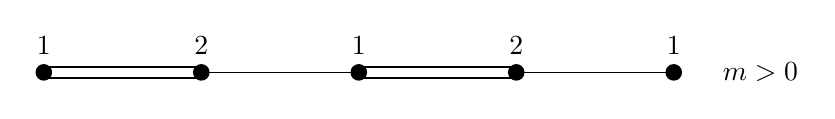
\begin{tikzpicture}
	\draw[double=none,double distance=3pt,thick] (2,0) -- (4,0);
	\draw[double=none,double distance=3pt,thick] (6,0) -- (8,0);
	\fill (2,0) circle (3pt) node[above,yshift=0.1cm] {$1$};
	\fill (4,0) circle (3pt) node[above,yshift=0.1cm] {$2$};
	\fill (6,0) circle (3pt) node[above,yshift=0.1cm] {$1$};
	\fill (8,0) circle (3pt) node[above,yshift=0.1cm] {$2$};
	\fill (10,0) circle (3pt) node[above,yshift=0.1cm] {$1$};
	\draw (4,0) -- (6,0);
	\draw (8,0) -- (10,0) node[right,xshift=0.5cm] {$m>0$};
\end{tikzpicture}
\end{center}
\begin{center}
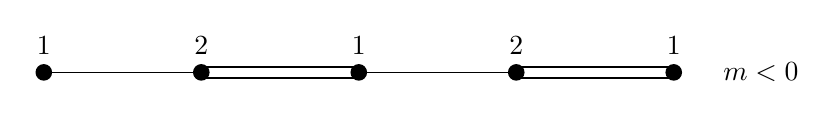
\begin{tikzpicture}
	\draw[double=none,double distance=3pt,thick] (4,0) -- (6,0);
	\draw[double=none,double distance=3pt,thick] (8,0) -- (10,0) node[right,xshift=0.5cm] {$m<0$};
	\fill (2,0) circle (3pt) node[above,yshift=0.1cm] {$1$};
	\fill (4,0) circle (3pt) node[above,yshift=0.1cm] {$2$};
	\fill (6,0) circle (3pt) node[above,yshift=0.1cm] {$1$};
	\fill (8,0) circle (3pt) node[above,yshift=0.1cm] {$2$};
	\fill (10,0) circle (3pt) node[above,yshift=0.1cm] {$1$};
	\draw (2,0) -- (4,0);
	\draw (6,0) -- (8,0);
\end{tikzpicture}
\end{center}

Joining the two states together
\begin{center}
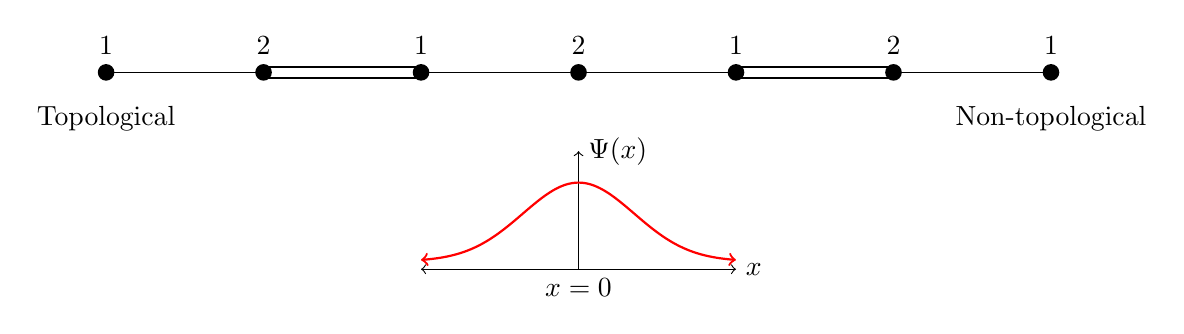
\begin{tikzpicture}
	\draw[double=none,double distance=3pt,thick] (2,0) -- (4,0);
	\draw[double=none,double distance=3pt,thick] (8,0) -- (10,0);
	\fill (0,0) circle (3pt) node[above,yshift=0.1cm] {$1$} node[below,yshift=-0.3cm] {Topological};
	\fill (2,0) circle (3pt) node[above,yshift=0.1cm] {$2$};
	\fill (4,0) circle (3pt) node[above,yshift=0.1cm] {$1$};
	\fill (6,0) circle (3pt) node[above,yshift=0.1cm] {$2$};
	\fill (8,0) circle (3pt) node[above,yshift=0.1cm] {$1$};
	\fill (10,0) circle (3pt) node[above,yshift=0.1cm] {$2$};
	\fill (12,0) circle (3pt) node[above,yshift=0.1cm] {$1$} node[below,yshift=-0.3cm] {Non-topological};
	\draw (0,0) -- (2,0);
	\draw (4,0) -- (6,0);
	\draw (6,0) -- (8,0);
	\draw (10,0) -- (12,0);
	\draw[<->] (4,-2.5) -- (8,-2.5) node[right] {$x$};
	\draw[<-] (6,-1) node[right] {$\Psi(x)$} -- (6,-2.5) node[below] {$x=0$};
	\draw[thick,domain=4:8,samples=200,red,<->] plot (\x, {e^(-(\x-6)^2)-2.4});
\end{tikzpicture}
\end{center}

$\Psi(x)$ describes an electron localized on this atom 2. If we had chosen $\ket{z}=\ket{\dn}$, one would have obtaine the solution for atom 1. In this case, $\ket{\up}\equiv\ket{1}$ and $\ket{\dn}\equiv\ket{2}$. The transition between the topological and ordinary insulator may be described in terms of change of sign of the mass of a Dirac fermion. This is true for any dimension.

\subsection{Higher Dimensions}

\definition{A \ul{crystal} is an infinite periodic array of identical groups of atoms. The group of atoms being repeated is called a \ul{basis}, while the regular array of points in space to which the basis is attached to is called the \ul{Bravais lattice}.\\

Crystal = (Basis, Bravais lattice)
\begin{center}
\begin{tikzpicture}
	\foreach \i in {0,2,4}{
		\foreach \j in {2,4}{
			\fill (\i+0.2*\j,\j) circle (3pt);
		}
	}
	\foreach \i in{2,4}{
		\fill (\i,0) circle (3pt);
	}
	\node[right,xshift=0.5cm] at (4.8,4)
		{Bravais lattice};
	\draw[thick,->,shorten >=1mm] (2.4,2) -- node[left] {$\vec{a}_{2}$} (2.8,4);
	\draw[thick,->,shorten >=1mm] (2.4,2) -- node[below] {$\vec{a}_{1}$} (4.4,2);
	\draw (0,0) node[below left,yshift=-0.7cm,xshift=-0.7cm] {Basis} circle (25 pt);
	\fill[red] (0.5,0) circle (3pt);
	\fill[blue] (-0.25,0.433) circle (3pt);
	\fill[green] (-0.25,-0.433) circle (3pt);
\end{tikzpicture}
\end{center}
}\\
A Bravais lattice in 3D consists of all points of the form
\begin{equation}
\vec{R}=n_{1}\vec{a}_{1}+n_{2}\vec{a}_{2}+n_{3}\vec{a}_{3},\quad n_{i}\in\mathbb{Z}\quad\forall i\in\{1,2,3\}
\end{equation}
$\vec{R}$ are called \ul{lattice vectors}. $\vec{a}_{1}$, $\vec{a}_{2}$, and $\vec{a}_{3}$ are the \ul{primitive translation vectors}. The choice of primitive translation vectors is not unique. Usually, one chooses the primitive translation vectors that express the most symmetry.\\

The parallelepiped defined by the primitive translation vectors is the \ul{primitive unit cell}. It always contains exactly one Bravais lattice point. When translated by all lattice vectors, the primitive unit cell completely fills all space. Since primitive translation vectors are not unique, the primitive unit cell is not unique.\\

One special type of unit cell is the \ul{Wigner-Seitz unit cell}. The Wigner-Seitz unit cell about a Bravais lattice point is the region of space that is closer to this Bravais lattice point than any other Bravais lattice point. One can construct the Wigner-Seitz unit cell by:
\begin{enumerate}
	\item From a given lattice point, draw lines connecting this point to all nearby lattice points.
	\item Bisect each line orthogonally with a line (in 2D) or a plane (in 3D).
	\item The smallest volume enclosed by these lines or planes is the Wigner-Seitz unit cell.
\end{enumerate}
\begin{center}
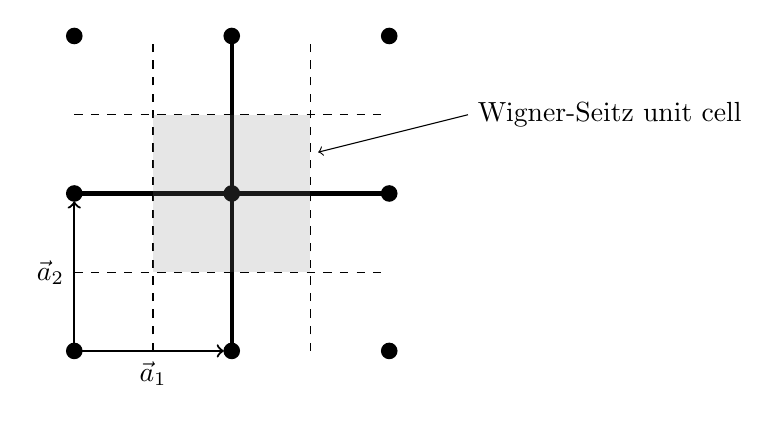
\begin{tikzpicture}
	\foreach \i in {0,2,4}{
		\foreach \j in {0,2,4}{
			\fill (\i,\j) circle (3pt);
		}
	}
	\draw[ultra thick] (2,0) -- (2,4);
	\draw[ultra thick] (0,2) -- (4,2);
	\draw[dashed] (1,0) -- (1,4);
	\draw[dashed] (3,0) -- (3,4);
	\draw[dashed] (0,3) -- (4,3);
	\draw[dashed] (0,1) -- (4,1);
	\draw[thick,->,shorten >=1mm] (0,0) -- node[left] {$\vec{a}_{2}$} (0,2);
	\draw[thick,->,shorten >=1mm] (0,0) -- node[below] {$\vec{a}_{1}$} (2,0);
	\fill[gray,fill opacity=0.2] (1,1) rectangle (3,3);
	\draw[->,shorten >=1mm] (5,3) node[right] {Wigner-Seitz unit cell} -- (3,2.5);
\end{tikzpicture}
\end{center}
Symmetry of the Wigner-Seitz unit cell is always the same as the symmetry of the Bravais lattice. It is also clear that it only contains one Bravais lattice point. Thus, the Wigner-Seitz unit cell is also a primitive unit cell.\\

\example{1}{When $\abs{\vec{a}_{1}}=\abs{\vec{a}_{2}}$ and the angle between $\vec{a}_{1}$ and $\vec{a}_{2}$ is $\frac{\pi}{2}$, the Bravais lattice is a square lattice.\\
\begin{center}
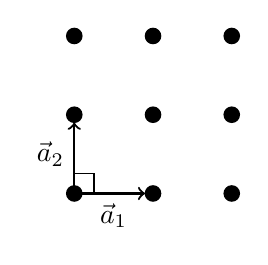
\begin{tikzpicture}
	\foreach \i in {0,1,2}{
		\foreach \j in {0,1,2}{
			\fill (\i,\j) circle (3pt);
		}
	}
	\draw[thick,->,shorten >=1mm] (0,0) -- node[left] {$\vec{a}_{2}$} (0,1);
	\draw[thick,->,shorten >=1mm] (0,0) -- node[below] {$\vec{a}_{1}$} (1,0);
	\draw (0,0.25) -- (0.25,0.25) -- (0.25,0);
\end{tikzpicture}
\end{center}
}

\example{2}{When $\abs{\vec{a}_{1}}=\abs{\vec{a}_{2}}$ and the angle between $\vec{a}_{1}$ and $\vec{a}_{2}$ is $\frac{\pi}{3}$, the Bravais lattice is a hexagonal (or triangular) lattice.\\
\begin{center}
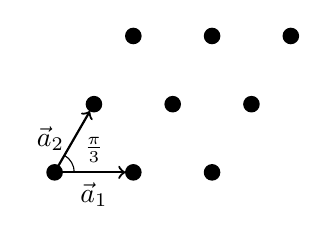
\begin{tikzpicture}
	\foreach \i in {0,1,2}{
		\foreach \j in {0,1,2}{
			\fill (\i+0.5*\j,0.866*\j) circle (3pt);
		}
	}
	\draw[thick,->,shorten >=1mm] (0,0) -- node[left] {$\vec{a}_{2}$} (0.5,0.866);
	\draw[thick,->,shorten >=1mm] (0,0) -- node[below] {$\vec{a}_{1}$} node[above,font=\footnotesize] {$\frac{\pi}{3}$} (1,0);
	\draw (0.25,0) arc (0:60:0.25);
\end{tikzpicture}
\end{center}
}

Consider the 2D honeycomb lattice structure, as in graphene.\\
\begin{center}
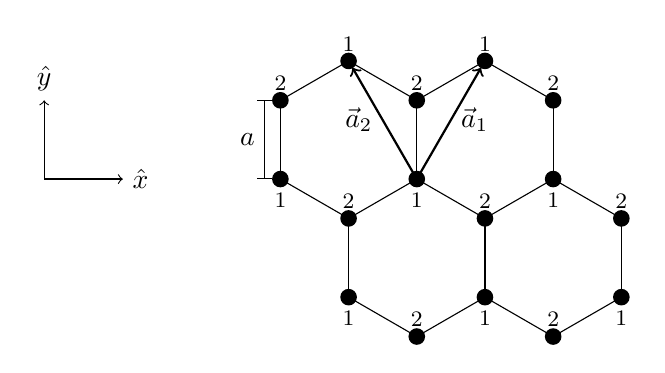
\begin{tikzpicture}
	\foreach \i in {0,1}{
		\fill (0.866+1.732*\i,1.5) circle (3pt);
	}
	\foreach \i in {0,1,2}{
		\foreach \j in {0,1}{
			\fill (1.732*\i,\j) circle (3pt);
		}
	}
	\foreach \i in {0,1,2}{
		\foreach \j in {0,1}{
			\fill (0.866+1.732*\i,-1.5+\j) circle (3pt);
		}
	}
	\foreach \i in {1,2}{
		\fill (1.732*\i,-2) circle (3pt);
	}
	\foreach \i in {0,1,2}{
		\draw (1.732*\i,0) -- (1.732*\i,1);
	}
	\foreach \i in {0,1,2}{
		\draw (0.866+1.732*\i,-1.5) -- (0.866+1.732*\i,-0.5);
	}
	\foreach \i in {0,1}{
		\draw (1.732*\i,1) -- (0.866+1.732*\i,1.5);
	}
	\foreach \i in {0,1}{
		\draw (0.866+1.732*\i,1.5) -- (1.732+1.732*\i,1);
	}
	\foreach \i in {0,1,2}{
		\draw (1.732*\i,0) -- (0.866+1.732*\i,-0.5);
	}
	\foreach \i in {0,1}{
		\draw (0.866+1.732*\i,-0.5) -- (1.732+1.732*\i,0);
	}
	\foreach \i in {0,1}{
		\draw (0.866+1.732*\i,-1.5) -- (1.732+1.732*\i,-2);
	}
	\foreach \i in {1,2}{
		\draw (1.732*\i,-2) -- (0.866+1.732*\i,-1.5);
	}
	\draw[thick,->,shorten >=1mm] (1.732,0) -- node[left] {$\vec{a}_{2}$} (0.866,1.5);
	\draw[thick,->,shorten >=1mm] (1.732,0) -- node[right] {$\vec{a}_{1}$} (2.598,1.5);
	\draw[|-|] (-0.2,0) -- node[left] {$a$} (-0.2,1);
	\foreach \i in {0,1}{
		\node[above,font=\footnotesize] at (0.866+1.732*\i,1.5) {1};
	}
	\foreach \i in {0,1,2}{
		\node[above,font=\footnotesize] at (1.732*\i,1) {2};
	}
	\foreach \i in {0,1,2}{
		\node[below,font=\footnotesize,yshift=-0.05cm] at (1.732*\i,0) {1};
	}
	\foreach \i in {0,1,2}{
		\node[above,font=\footnotesize] at (0.866+1.732*\i,-0.5) {2};
	}
	\foreach \i in {0,1,2}{
		\node[below,font=\footnotesize,yshift=-0.05cm] at (0.866+1.732*\i,-1.5) {1};
	}
	\foreach \i in {1,2}{
		\node[above,font=\footnotesize] at (1.732*\i,-2) {2};
	}
	\draw[->] (-3,0) -- (-2,0) node[right] {$\hat{x}$};
	\draw[->] (-3,0) -- (-3,1) node[above] {$\hat{y}$};
\end{tikzpicture}
\end{center}
Note that the points on this lattice do not form a Bravais lattice. However, if grouping atoms 1 and 2, the Bravais lattice is hexagonal. Thus, this honeycomb lattice is a hexagonal Bravais lattice with a two-atom basis. Let $a$ be the lattice constant of the hexagonal Bravais lattice. The primitive translation vectors are
\begin{equation}
\vec{a}_{1}=\frac{a}{2}(\hat{x}+\sqrt{3}\hat{y})\quad\trm{and}\quad\vec{a}_{2}=\frac{a}{2}(-\hat{x}+\sqrt{3}\hat{y})
\end{equation}
Another important concept to introduce is that of the \ul{reciprocal space} and \ul{reciprocal lattice}. In the 1D chain example, the Bloch states were introduced as
\begin{equation}
\ket{k}=\frac{1}{\sqrt{N}}\sum_{n}\ket{n}e^{ikna}
\end{equation}
An important property of the crystal momentum $k$ is that it is defined in the first Brillouin zone
\begin{equation}
\ket{k+\frac{2\pi}{a}m}=\ket{k}\quad\forall m\in\mathbb{Z},\quad\trm{since }e^{i\left(\frac{2\pi}{a}m\right)(na)}=1
\end{equation}
This can be generalized to higher dimensions.\\

Let us introduce the \ul{reciprocal lattice vectors} $\vec{G}$ which are defined by
\begin{equation}
e^{i\vec{G}\cdot\vec{R}}=1
\end{equation}
where $\vec{R}=n_{1}\vec{a}_{1}+n_{2}\vec{a}_{2}+n_{3}\vec{a}_{3},\quad n_{i}\in\mathbb{Z}\quad\forall i\in\{1,2,3\}$ are the Bravais lattice vectors. In the 1D case, $\frac{2\pi}{a}m$ took on the role of $\vec{G}$ while $na$ took on the role of $\vec{R}$. In analogy to $\vec{R}$ which indexes lattice points in real space, one can define the reciprocal lattice to be indexed by $\vec{G}$, where $\vec{G}$ is written as
\begin{equation}
\vec{G}=m_{1}\vec{b}_{1}+m_{2}\vec{b}_{2}+m_{3}\vec{b}_{3},\quad m_{1},m_{2},m_{3}\in\mathbb{Z}
\end{equation}
where $\vec{b}_{1}$, $\vec{b}_{2}$, and $\vec{b}_{3}$ are the \ul{primitive translation vectors of the reciprocal lattice}. In order to have $e^{i\vec{G}\cdot\vec{R}}=1$, one requires that $\vec{G}\cdot\vec{R}$ is an integer multiple of $2\pi$ for any $\vec{G}$ and $\vec{R}$. This is satisfied if
\begin{equation}
\vec{b}_{i}\cdot\vec{a}_{j}=2\pi\delta_{ij}
\end{equation}
Thus
\begin{equation}
\begin{aligned}
\vec{G}\cdot\vec{R}&=(m_{1}\vec{b}_{1}+m_{2}\vec{b}_{2}+m_{3}\vec{b}_{3})\cdot(n_{1}\vec{a}_{1}+n_{2}\vec{a}_{2}+n_{3}\vec{a}_{3})\\
&=2\pi(m_{1}n_{1}+m_{2}n_{2}+m_{3}n_{3})\\
&=2\pi(\trm{integer})\\
\implies e^{i\vec{G}\cdot\vec{R}}&=1
\end{aligned}
\end{equation}

One can explicitly construct $\vec{b}_{i}$ as
\begin{equation}
\begin{aligned}
\vec{b}_{1}&=\frac{2\pi}{V_{c}}(\vec{a}_{2}\times\vec{a}_{3})\\
\vec{b}_{2}&=\frac{2\pi}{V_{c}}(\vec{a}_{3}\times\vec{a}_{1})\\
\vec{b}_{3}&=\frac{2\pi}{V_{c}}(\vec{a}_{1}\times\vec{a}_{2})\\
\end{aligned}
\end{equation}
where
\begin{equation}
V_{c}=\vec{a}_{1}\cdot(\vec{a}_{2}\times\vec{a}_{3})
\end{equation}
is the volume of the unit cell. In the 2D case, replace one of the $\vec{a}_{i}$ with the unit vector normal to the plane defined by the primitive translation vectors (e.g. $\vec{a}_{3}=\hat{z}$). Note in the 1D example, $b=\frac{2\pi}{a}$.\\

The first Brillouin zone is the Wigner-Seitz unit cell of the reciprocal lattice. The crystal momentum $\vec{k}$ was defined only in the first Brillouin zone.
\begin{equation}
\vec{k}=k_{1}\vec{b}_{1}+k_{2}\vec{b}_{2}+k_{3}\vec{b}_{3}
\end{equation}
The Brillouin zone boundaries correspond to $k_{i}=\pm\frac{1}{2}$ given that the Brillouin zone about a reciprocal lattice point can be constructed by bisecting the primitive translation vectors of the reciprocal lattice.\\

Let us find the first Brillouin zone of graphene.\\
\begin{center}
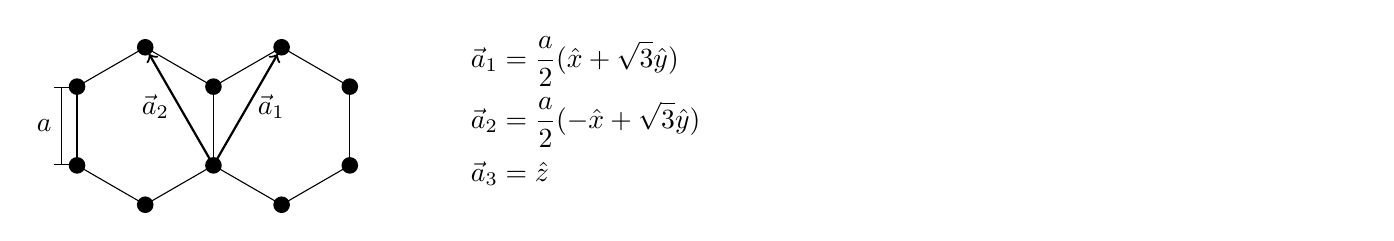
\begin{tikzpicture}
	\foreach \i in {0,1}{
		\fill (0.866+1.732*\i,1.5) circle (3pt);
	}
	\foreach \i in {0,1,2}{
		\foreach \j in {0,1}{
			\fill (1.732*\i,\j) circle (3pt);
		}
	}
	\foreach \i in {0,1}{
		\fill (0.866+1.732*\i,-0.5) circle (3pt);
	}
	\foreach \i in {0,1,2}{
		\draw (1.732*\i,0) -- (1.732*\i,1);
	}
	\foreach \i in {0,1}{
		\draw (1.732*\i,1) -- (0.866+1.732*\i,1.5);
	}
	\foreach \i in {0,1}{
		\draw (0.866+1.732*\i,1.5) -- (1.732+1.732*\i,1);
	}
	\foreach \i in {0,1}{
		\draw (1.732*\i,0) -- (0.866+1.732*\i,-0.5);
	}
	\foreach \i in {0,1}{
		\draw (0.866+1.732*\i,-0.5) -- (1.732+1.732*\i,0);
	}
	\draw[thick,->,shorten >=1mm] (1.732,0) -- node[left] {$\vec{a}_{2}$} (0.866,1.5);
	\draw[thick,->,shorten >=1mm] (1.732,0) -- node[right] {$\vec{a}_{1}$} (2.598,1.5);
	\draw[|-|] (-0.2,0) -- node[left] {$a$} (-0.2,1);
	\node[anchor=north west,right] at (4,0.65)
		{\[
			\begin{aligned}
			\vec{a}_{1}&=\frac{a}{2}(\hat{x}+\sqrt{3}\hat{y})\\
			\vec{a}_{2}&=\frac{a}{2}(-\hat{x}+\sqrt{3}\hat{y})\\
			\vec{a}_{3}&=\hat{z}\\
			\end{aligned}
		\]};
\end{tikzpicture}
\end{center}
\begin{equation}
\begin{aligned}
V_{c}&=\vec{a}_{1}\cdot(\vec{a}_{2}\times\vec{a}_{3})
=\vec{a}_{3}\cdot(\vec{a}_{1}\times\vec{a}_{2})
=\hat{z}\cdot\left[\frac{a^{2}\sqrt{3}}{4}(\hat{x}\times\hat{y}-\hat{y}\times\hat{x})\right]
=\frac{a^{2}\sqrt{3}}{2}\\
\vec{b}_{1}&=\frac{2\pi}{V_{c}}(\vec{a}_{2}\times\vec{a}_{3})=\left(\frac{4\pi}{a^{2}\sqrt{3}}\right)\left(\frac{a}{2}\right)(-\hat{x}\times\hat{z}+\sqrt{3}\hat{y}\times\hat{z})=\frac{2\pi}{a}\left(\hat{x}+\frac{1}{\sqrt{3}}\hat{y}\right)\\
\vec{b}_{2}&=\frac{2\pi}{V_{c}}(\vec{a}_{2}\times\vec{a}_{3})=\left(\frac{4\pi}{a^{2}\sqrt{3}}\right)\left(\frac{a}{2}\right)(\hat{z}\times\hat{x}+\hat{z}\times\sqrt{3}\hat{y})=\frac{2\pi}{a}\left(-\hat{x}+\frac{1}{\sqrt{3}}\hat{y}\right)\\
\end{aligned}
\end{equation}
Note that $\vec{b}_{1}$ and $\vec{b}_{2}$ satisfy $\vec{b}_{i}\cdot\vec{a}_{j}=2\pi\delta_{ij}$. Similarly, $\abs{\vec{b}_{1}}=\abs{\vec{b}_{2}}$ and the angle between them is $\frac{\pi}{3}$. Thus, the reciprocal lattice is also hexagonal and the first Brillouin zone is also a hexagon.

\subsection{Electronic Structure}
Before considering the electronic structure of graphene, let us consider the electronic structure of the square lattice as a warm-up example. Let there be one atom per unit cell.
\begin{center}
\begin{tikzpicture}
	\foreach \i in {0,2,4}{
		\foreach \j in {0,2,4}{
			\fill (\i,\j) circle (3pt);
		}
	}
	\draw[decorate,decoration={coil,aspect=0}] (2,0) -- node[right] {$t$} (2,2);
	\draw[decorate,decoration={coil,aspect=0}] (2,2) -- node[right] {$t$} (2,4);
	\draw[decorate,decoration={coil,aspect=0}] (0,2) -- node[above] {$t$} (2,2);
	\draw[decorate,decoration={coil,aspect=0}] (2,2) -- node[above] {$t$} (4,2);
	\draw[thick,->,shorten >=1mm] (0,0) -- node[left] {$\vec{a}_{2}$} (0,2);
	\draw[thick,->,shorten >=1mm] (0,0) -- node[below] {$\vec{a}_{1}$} (2,0);
	\draw[|-|] (2,-0.3) -- node[below] {$a$} (4,-0.3);
	\node[anchor=north west,right] at (4,3.5)
		{\[
			\begin{aligned}
			\vec{a}_{1}&=a\hat{x},&\quad\vec{a}_{2}&=a\vec{y}\\
			\vec{b}_{1}&=\frac{2\pi}{a}\hat{x},&\quad\vec{b}_{2}&=\frac{2\pi}{a}\vec{y}\\
			\end{aligned}
		\]};
	\draw[->] (5,0) -- (5,1) node[above] {$\hat{y}$};
	\draw[->] (5,0) -- (6,0) node[right] {$\hat{x}$};
\end{tikzpicture}
\end{center}
Assuming the tight-binding model, the Hamiltonian is written as
\begin{equation}
H=-t\sum_{\vec{R},\vec{a}}\left(\ketbra*{\vec{R}+\vec{a}}{\vec{R}}+\ketbra*{\vec{R}}{\vec{R}+\vec{a}}\right)
\end{equation}
where $\vec{a}\in\{\vec{a}_{1},\vec{a}_{2}\}$. One sums over $\vec{R}+\vec{a}$ and not $\vec{R}-\vec{a}$ to avoid double-counting of possible transitions. To diagonalize this Hamiltonian, let us use the inverse lattice Fourier transform.
\begin{equation}
\begin{aligned}
\ket*{\vec{R}}&=\sum_{\vec{k}}\ket*{\vec{k}}\braket*{\vec{k}}{\vec{R}}\\
&=\frac{1}{\sqrt{N}}\sum_{\vec{k}}e^{-i\vec{k}\cdot\vec{R}}\ket*{\vec{k}}
\end{aligned}
\end{equation}
where $\vec{k}=k_{1}\vec{b}_{1}+k_{2}\vec{b}_{2}$ is restricted to the first Brillouin zone $(-\frac{1}{2}\leq k_{1},k_{2}<\frac{1}{2})$. The Hamiltonian can now be written as
\begin{equation}
\begin{aligned}
H&=-t\left(\frac{1}{N}\right)\sum_{\vec{R},\vec{a}}\sum_{\vec{k},\vec{k}'}\left(\ketbra*{\vec{k}}{\vec{k}'}e^{-i\vec{k}\cdot\left(\vec{R}+\vec{a}\right)}e^{i\vec{k}'\cdot\vec{R}}+\ketbra*{\vec{k}}{\vec{k}'}e^{-i\vec{k}\cdot\vec{R}}e^{i\vec{k}'\cdot\left(\vec{R}+\vec{a}\right)}\right)\\
&=-t\sum_{\vec{k},\vec{a}}\ketbra*{\vec{k}}{\vec{k}}\left(e^{-i\vec{k}\cdot\vec{a}}+e^{i\vec{k}\cdot\vec{a}}\right)\\
&\quad\explain\trm{ Since }\frac{1}{N}\sum_{\vec{R}}e^{-i\left(\vec{k}-\vec{k}'\right)\cdot\vec{R}}=\delta_{\vec{k}\vec{k}'}\\
&=-2t\sum_{\vec{k},\vec{a}}\cos\left(\vec{k}\cdot\vec{a}\right)\ketbra*{\vec{k}}{\vec{k}}\\
&=\sum_{\vec{k}}H(\vec{k})\ketbra*{\vec{k}}{\vec{k}}
\end{aligned}
\end{equation}

Thus, the band dispersion is
\begin{equation}
\varepsilon(\vec{k})=-2t\sum_{\vec{a}}\cos\left(\vec{k}\cdot\vec{a}\right)=-2t\left[\cos(k_{x}a)+\cos(k_{y}a)\right]
\end{equation}

Thus, there is a minimum of $\varepsilon_{\trm{min}}=-4t$ at $k_{x}=k_{y}=0$ (or $\vec{k}=\vec{0}$). Likewise, there is a maximum of $\varepsilon_{\trm{max}}=4t$ at the Brillouin zone corners $k_{x},k_{y}=\pm\frac{\pi}{a}$. The bandwidth is $\varepsilon_{\trm{max}}-\varepsilon_{\trm{min}}=8t$.\\
\begin{center}
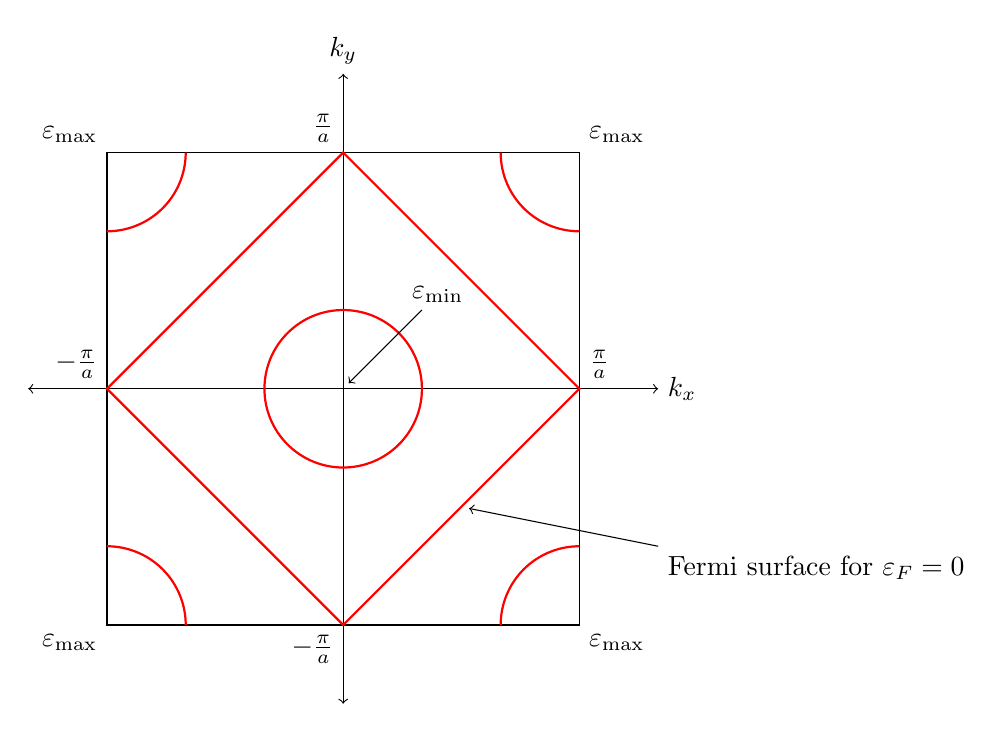
\begin{tikzpicture}
	\draw[<->] (-4,0) -- (4,0) node[right] {$k_{x}$};
	\draw[<->] (0,-4) -- (0,4) node[above] {$k_{y}$};
	\draw (-3,3) node[above left] {$\varepsilon_{\trm{max}}$} -- node[above left] {$\frac{\pi}{a}$} (3,3) node[above right] {$\varepsilon_{\trm{max}}$} -- node[above right] {$\frac{\pi}{a}$} (3,-3) node[below right] {$\varepsilon_{\trm{max}}$} -- node[below left] {$-\frac{\pi}{a}$}(-3,-3) node[below left] {$\varepsilon_{\trm{max}}$} -- node[above left] {$-\frac{\pi}{a}$} cycle;
	\draw[red,thick] (-3,0) -- (0,3) -- (3,0) -- (0,-3) -- cycle;
	\draw[red,thick] (0,0) circle (1cm);
	\draw[red,thick,domain=0:90,samples=200] plot ({cos(\x)-3},{sin(\x)-3});
	\draw[red,thick,domain=90:180,samples=200] plot ({cos(\x)+3},{sin(\x)-3});
	\draw[red,thick,domain=180:270,samples=200] plot ({cos(\x)+3},{sin(\x)+3});
	\draw[red,thick,domain=270:360,samples=200] plot ({cos(\x)-3},{sin(\x)+3});
	\draw[->,shorten >=1mm] (1,1) node[yshift=0.2cm,xshift=0.2cm] {$\varepsilon_{\trm{min}}$} -- (0,0);
	\draw[->,shorten >=1mm] (4,-2) node[below right] {Fermi surface for $\varepsilon_{F}=0$} -- (1.5,-1.5);
\end{tikzpicture}
\end{center}

\begin{figure}[H]
	\centering
	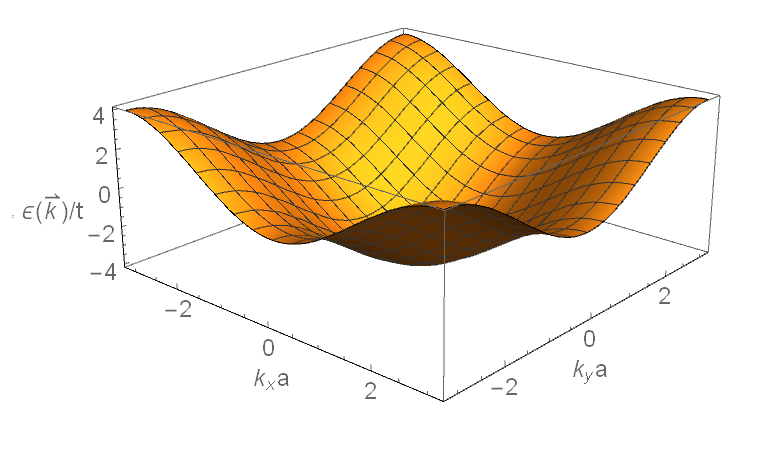
\includegraphics[width=\textwidth]{Images/2/square_lattice_band.png}
	\caption{Energy band of square lattice}
\end{figure}

Expand $\varepsilon(\vec{k})$ in terms of $\vec{k}$ near the minimum to second order.
\begin{equation}
\begin{aligned}
\varepsilon(\vec{k})&\approx-2t\left[1-\frac{1}{2}(k_{x}a)^{2}+1-\frac{1}{2}(k_{y}a)^{2}\right]\\
&=-4t+ta^{2}(k_{x}^{2}+k_{y}^{2})\\
&=-4t+ta^{2}k^{2}
\end{aligned}
\end{equation}

This resembles the dispersion relation for a free electron $\varepsilon(\vec{k})=\frac{\hbar^{2}k^{2}}{2m}$. One can define an effective mass $m^{*}$ as follows
\begin{equation}
\varepsilon(\vec{k})-\varepsilon_{\trm{min}}=ta^{2}k^{2}=\frac{\hbar^{2}k^{2}}{2m^{*}}
\end{equation}
such that
\begin{equation}
m^{*}=\frac{\hbar^{2}}{2ta^{2}}
\end{equation}
The Fermi surface be found as a solution to
\begin{equation}
\varepsilon(\vec{k})=\varepsilon_{F},\quad -4t\leq\varepsilon_{F}\leq4t
\end{equation}
When $\varepsilon_{F}$ is near the bottom of the band, one has
\begin{equation}
\begin{aligned}
-4t+\frac{\hbar^{2}k^{2}}{2m^{*}}&=\varepsilon_{F}
k_{x}^{2}+k_{y}^{2}=\frac{2m^{*}}{\hbar^{2}}(\varepsilon_{F}+4t)
\end{aligned}
\end{equation}
This is the equation of a circle with radius $k_{F}=\sqrt{\frac{2m^{*}}{\hbar^{2}}(\varepsilon_{F}+4t)}$. Note this only applies near the minimum energy level.\\

The number of possible states per band is $2N$. When it is half-filled, there is one free electron per atom. Since $\varepsilon(\vec{k})$ is symmetric around zero energy, it is clear $\varepsilon_{F}=0$ when the band is half-filled.\\

Let us now consider the electronic structure of graphene.
\begin{center}
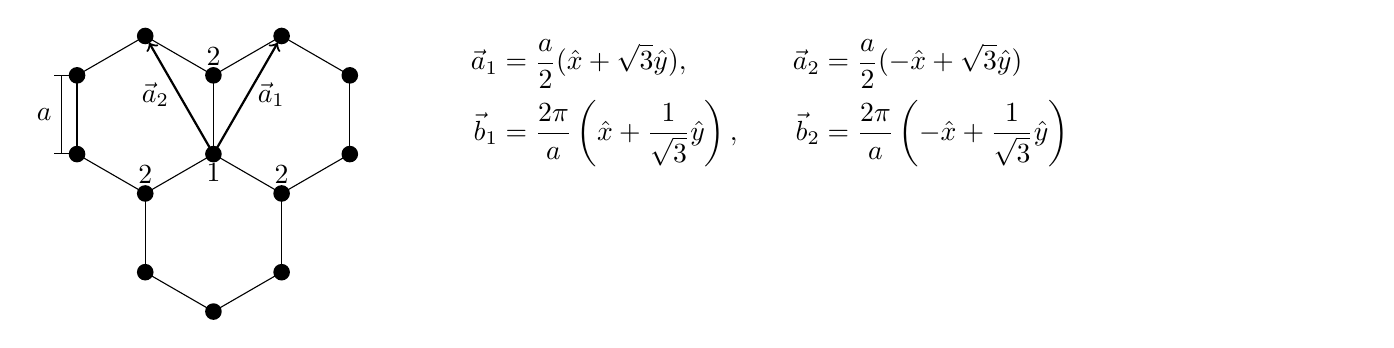
\begin{tikzpicture}
	\foreach \i in {0,1}{
		\fill (0.866+1.732*\i,1.5) circle (3pt);
	}
	\foreach \i in {0,1,2}{
		\foreach \j in {0,1}{
			\fill (1.732*\i,\j) circle (3pt);
		}
	}
	\foreach \i in {0,1}{
		\foreach \j in{0,1}{
			\fill (0.866+1.732*\i,-1.5+\j) circle (3pt);
		}
	}
	\fill (1.732,-2) circle (3pt);
	\foreach \i in {0,1,2}{
		\draw (1.732*\i,0) -- (1.732*\i,1);
	}
	\foreach \i in {0,1}{
		\draw (1.732*\i,1) -- (0.866+1.732*\i,1.5);
	}
	\foreach \i in {0,1}{
		\draw (0.866+1.732*\i,1.5) -- (1.732+1.732*\i,1);
	}
	\foreach \i in {0,1}{
		\draw (1.732*\i,0) -- (0.866+1.732*\i,-0.5);
	}
	\foreach \i in {0,1}{
		\draw (0.866+1.732*\i,-0.5) -- (1.732+1.732*\i,0);
	}
	\foreach \i in {0,1}{
		\draw (0.866+1.732*\i,-1.5) -- (0.866+1.732*\i,-0.5);
	}
	\foreach \i in {0,1}{
		\draw (1.732,-2) -- (0.866+1.732*\i,-1.5);
	}
	\node[above] at (1.732,1) {2};
	\node[below] at (1.732,0) {1};
	\foreach \i in {0,1}{
		\node[above] at (0.866+1.732*\i,-0.5) {2};
	}
	\draw[thick,->,shorten >=1mm] (1.732,0) -- node[left] {$\vec{a}_{2}$} (0.866,1.5);
	\draw[thick,->,shorten >=1mm] (1.732,0) -- node[right] {$\vec{a}_{1}$} (2.598,1.5);
	\draw[|-|] (-0.2,0) -- node[left] {$a$} (-0.2,1);
	\node[anchor=north west,right] at (4,0.65)
		{\[
			\begin{aligned}
			\vec{a}_{1}&=\frac{a}{2}(\hat{x}+\sqrt{3}\hat{y}),&\quad\vec{a}_{2}&=\frac{a}{2}(-\hat{x}+\sqrt{3}\hat{y})\\
			\vec{b}_{1}&=\frac{2\pi}{a}\left(\hat{x}+\frac{1}{\sqrt{3}}\hat{y}\right),&\quad\vec{b}_{2}&=\frac{2\pi}{a}\left(-\hat{x}+\frac{1}{\sqrt{3}}\hat{y}\right)\\
			\end{aligned}
		\]};
\end{tikzpicture}
\end{center}

Assuming the tight-binding approximation
\begin{equation}
H=-t\sum_{\vec{k}}\left(\ketbra*{\vec{R},2}{\vec{R},1}+\ketbra*{\vec{R}-\vec{a}_{1},2}{\vec{R},1}+\ketbra*{\vec{R}-\vec{a}_{2},2}{\vec{R},1}+\tikzmarknode{HC}{\trm{h.c.}}\right)
\end{equation}
\begin{tikzpicture}[overlay,remember picture,shorten <=1mm,font=\footnotesize]
	\draw[red,<-] (HC.south) -- ++ (0,-0.5) node[below,yshift=0.1cm] {Hermitian conjugate};
\end{tikzpicture}
The inverse lattice Fourier transform gives in reciprocal space
\begin{equation}
\ket*{\vec{R},\alpha}=\frac{1}{\sqrt{N}}\sum_{\vec{R}}\ket*{\vec{k},\alpha}e^{-i\vec{k}\cdot\vec{R}},\quad\alpha\in\{1,2\}
\end{equation}
Thus
\begin{equation}
\begin{aligned}
H&=-t\left(\frac{1}{N}\right)\sum_{\vec{R}}\sum_{\vec{k},\vec{k}'}\bigg[\ketbra*{\vec{k},2}{\vec{k}',1}e^{-i\left(\vec{k}-\vec{k}'\right)\cdot\vec{R}}+\ketbra*{\vec{k},2}{\vec{k}',1}e^{-i\vec{k}\cdot\left(\vec{R}-\vec{a}_{1}\right)}e^{i\vec{k}'\cdot\vec{R}}\\
&\qquad\qquad\qquad\qquad\qquad+\ketbra*{\vec{k},2}{\vec{k}',1}e^{-i\vec{k}\cdot\left(\vec{R}-\vec{a}_{2}\right)}e^{i\vec{k}'\cdot\vec{R}}+\trm{h.c.}\bigg]\\
&=-t\sum_{\vec{k}}\left[\ketbra*{\vec{k},2}{\vec{k},1}\left(1+e^{i\vec{k}\cdot\vec{a}_{1}}+e^{i\vec{k}\cdot\vec{a}_{2}}\right)+\ketbra*{\vec{k},1}{\vec{k},2}\left(1+e^{-i\vec{k}\cdot\vec{a}_{1}}+e^{-i\vec{k}\cdot\vec{a}_{2}}\right)\right]\\
&\quad\explain\trm{ Since }\frac{1}{N}\sum_{\vec{R}}e^{-i\left(\vec{k}-\vec{k}'\right)\cdot\vec{R}}=\delta_{\vec{k}\vec{k}'}\\
&=\sum_{\vec{k}}H(\vec{k})
\end{aligned}
\end{equation}
Invoking pseudospin states $\ket*{\vec{k},1}\equiv\ket{1}$ as $\ket{\up}$ and $\ket*{\vec{k},2}\equiv\ket{2}$ as $\ket{\dn}$, one can write
\begin{equation}
H(\vec{k})=\vec{d}(\vec{k})\cdot\vec{\sigma}
\end{equation}
where $\vec{d}(\vec{k})$ is described by
\begin{equation}
\begin{aligned}
d_{x}(\vec{k})&=-t\left[1+\cos(\vec{k}\cdot\vec{a}_{1})+\cos(\vec{k}\cdot\vec{a}_{2})\right]\\
d_{y}(\vec{k})&=-t\left[\sin(\vec{k}\cdot\vec{a}_{1})+\sin(\vec{k}\cdot\vec{a}_{2})\right]\\
d_{z}(\vec{k})&=0
\end{aligned}
\end{equation}
This gives eigenvalues $\varepsilon_{\pm}(\vec{k})=\pm\abs*{\vec{d}(\vec{k})}$.\\

In undoped graphene, there is one valence electron per carbon atom. Given that there are two carbon atoms per basis and there are $N$ primitive unit cells, there are $2N$ valence electrons available. Since there are $2N$ possible states per band, the lower band is completely filled while the upper band is empty. This wuld suggest that graphene is an insulator. In reality, the situation is more complicated.\\

In order to analyze the band dispersion, let us rewrite $\vec{k}$, which is currently expressed in terms of $\vec{b}_{1}$ and $\vec{b}_{2}$, in terms of $\hat{x}$ and $\hat{y}$.
\begin{equation}
\begin{aligned}
\vec{k}&=k_{1}\vec{b}_{1}+k_{2}\vec{b}_{2}\\
\vec{k}\cdot\vec{a}_{1}&=(k_{1}\vec{b}_{1}+k_{2}\vec{b}_{2})\cdot\vec{a}_{1}=2\pi k_{1}\\
&=(k_{x}\hat{x}+k_{y}\hat{y})\cdot\frac{a}{2}(\hat{x}+\sqrt{3}\hat{y})=\frac{a}{2}(k_{x}+\sqrt{3}k_{y})\\
\vec{k}\cdot\vec{a}_{2}&=(k_{1}\vec{b}_{1}+k_{2}\vec{b}_{2})\cdot\vec{a}_{2}=2\pi k_{2}\\
&=(k_{x}\hat{x}+k_{y}\hat{y})\cdot\frac{a}{2}(-\hat{x}+\sqrt{3}\hat{y})=\frac{a}{2}(-k_{x}+\sqrt{3}k_{y})\\
\end{aligned}
\end{equation}
Therefore
\begin{equation}
k_{1}=\frac{a}{4\pi}(k_{x}+\sqrt{3}k_{y})\quad\trm{and}\quad k_{2}=\frac{a}{4\pi}(-k_{x}+\sqrt{3}k_{y})
\end{equation}

Thus, $\vec{d}(\vec{k})$ becomes
\begin{equation}
\begin{aligned}
d_{x}(\vec{k})&=-t\left[1+2\cos\left(\frac{k_{x}a}{2}\right)\cos\left(\frac{\sqrt{3}k_{y}a}{2}\right)\right]\\
d_{y}(\vec{k})&=-2t\cos\left(\frac{k_{x}a}{2}\right)\sin\left(\frac{\sqrt{3}k_{y}a}{2}\right)\\
d_{z}(\vec{k})&=0
\end{aligned}
\end{equation}

By inspection, there are two points (and only two points) in the first Brillouin zone such that $\abs*{\vec{d}(\vec{k})}=0$. Labeling these points as $\vec{k}_{\pm}$
\begin{equation}
\begin{aligned}
\vec{k}_{+}&=\left(\frac{4\pi}{3a},0\right)\\
\vec{k}_{-}&=\left(-\frac{4\pi}{3a},0\right)
\end{aligned}
\end{equation}
Let us construct the first Brillouin zone.
\begin{equation}
\vec{b}_{1}=\frac{2\pi}{a}\left(\hat{x}+\frac{1}{\sqrt{3}}\hat{y}\right)\quad\trm{and}\quad\vec{b}_{2}=\frac{2\pi}{a}\left(-\hat{x}+\frac{1}{\sqrt{3}}\hat{y}\right)
\end{equation}
Note that $\abs*{\vec{b}_{1}}=\abs*{\vec{b}_{2}}=\frac{2\pi}{a}\sqrt{1+\frac{1}{3}}=\frac{4\pi}{a\sqrt{3}}$ and $\cos\theta=\frac{\vec{b}_{1}\cdot\hat{x}}{\abs*{\vec{b}_{1}}}=\frac{\sqrt{3}}{2}$. Thus, $\vec{b}_{1}$ makes an angle of $\frac{\pi}{6}$ with the $x$-axis. Similarly, $\vec{b}_{2}$ makes an angle $\frac{5\pi}{6}$ with the $x$-axis. Note also that $\abs*{\vec{b}_{1}+\vec{b}_{2}}=\frac{4\pi}{a\sqrt{3}}$.
\begin{center}
\begin{tikzpicture}
	\draw[<->] (-4,0) -- (4,0) node[right] {$k_{x}$};
	\draw[<->] (0,-4) -- (0,4) node[above] {$k_{y}$};
	\node[regular polygon,regular polygon sides=6,minimum size=3.464cm,draw] at (0,0) {};
	\draw[ultra thick,->] (0,0) -- (90:3cm) node[right] {$\vec{b}_{1}+\vec{b}_{2}$};
	\draw[ultra thick,->] (0,0) -- (30:3cm) node[right] {$\vec{b}_{1}$};
	\draw[ultra thick,->] (0,0) -- (150:3cm) node[left] {$\vec{b}_{2}$};
	\draw[ultra thick,->] (0,0) -- (270:3cm) node[right] {$-\vec{b}_{1}-\vec{b}_{2}$};
	\draw[ultra thick,->] (0,0) -- (210:3cm) node[left] {$-\vec{b}_{1}$};
	\draw[ultra thick,->] (0,0) -- (330:3cm) node[right] {$-\vec{b}_{2}$};
	\fill (0,0) circle (4pt);
	\node[anchor=north west,right] at (4,0)
		{\[\ket*{\vec{k}+\vec{b}_{i}}=\ket*{\vec{k}}\]};
\end{tikzpicture}
\end{center}
Note that the corners of the Brillouin zone lying on the $x$-axis can be found through $\frac{\abs*{\vec{b}_{1}}}{2}\frac{1}{\cos\left(\frac{\pi}{6}\right)}=\frac{4\pi}{3a}$. Thus, $\vec{k}_{+}$ and $\vec{k}_{-}$ correspond to these two Brillouin zone corners. The other corners can be obtained from these two by adding reciprocal lattice vectors. Thus, $d_{x}(\vec{k})=d_{y}(\vec{k})=0$ at these corners and $\varepsilon_{+}=\varepsilon_{-}$ (i.e. conduction and valence bands touch at these points).
\begin{center}
\begin{tikzpicture}
	\draw[dashed,<->] (-2*pi,0) -- (2*pi,0) node[right] {$\varepsilon_{F}=0$};
	\draw[thick,<->,domain=-1.6*pi:1.6*pi,samples=200] node[above,yshift=1.4cm] {$\varepsilon_{+}$} plot (\x, {0.5*abs(1+2*cos(deg(\x/2)))});
	\draw[thick,<->,domain=-1.6*pi:1.6*pi,samples=200] node[below,yshift=-1.5cm] {$\varepsilon_{-}$} plot (\x, {-0.5*abs(1+2*cos(deg(\x/2)))});
	\fill[red] (-4*pi/3,0) circle (3pt) node[above] {$\vec{k}_{-}$};
	\fill[red] (4*pi/3,0) circle (3pt) node[above] {$\vec{k}_{+}$};
\end{tikzpicture}
\end{center}
Thus, graphene is known as a zero-gap insulator or a \ul{semimetal}. It is not simply a metal, since the Fermi surface is shrunk to a point. Similarly, it is not simply an insulator because there is no gap between the conduction and valence band. We shall characterize semimetals as the limit of metals as its Fermi surface is shrunk to a point. Similarly, we shall also characterize semimetals in the limit fo the band gap going to zero.\\

Note that the states most important at describing the electronic structure are the ones near the Fermi energy $\varepsilon_{F}$, as they are the states most strongly affected by perturbations. Let us expand near the points where the bands touch.
\begin{equation}
k_{x}\approx k_{\pm,x}+\delta k_{x}\quad\trm{and}\quad k_{y}\approx\delta k_{y},\trm{ where } k_{\pm,x}=\pm\frac{4\pi}{3a}
\end{equation}
Taking $\delta k_{x}$ and $\delta k_{y}$ to be small
\begin{equation}
\begin{aligned}
d_{\pm}^{x}(\vec{k})&\approx\pm\frac{\sqrt{3}}{2}ta\delta k_{x}\\
d_{\pm}^{y}(\vec{k})&\approx\frac{\sqrt{3}}{2}ta\delta k_{y}
\end{aligned}
\end{equation}

Let the Fermi velocity $v_{F}$ be defined as $\frac{\sqrt{3}ta}{2\hbar}$. The Hamiltonian then takes on the form
\begin{equation}
H_{\pm}(\vec{k})=\hbar v_{F}(\pm k_{x}\sigma^{x}+k_{y}\sigma^{y})
\end{equation}
where $\delta k_{x}$ and $\delta k_{y}$ have been replaced by $k_{x}$ and $k_{y}$ as it is understood that we are describing states near $\varepsilon_{F}=0$. We can also shift coordinates such that $k_{\pm,x}=0$ for each of the + and -- cases. The Hamiltonian now takes on the form of a Dirac Hamiltonian for a massless relativistic particle in 2D.\\

Diagonalizing the Hamiltonian to get the band dispersions
\begin{equation}
\varepsilon_{\pm}(\vec{k})=\pm\hbar v_{F}k=\pm\hbar v_{F}\sqrt{k_{x}^{2}+k_{y}^{2}}
\end{equation}
This dispersion resembles that of a massless particle with energy $E=\sqrt{p^{2}c^{2}+m^{2}c^{4}}=\approx pc$ (ultrarelativistic limit) in that both are linear in $k$.
\begin{center}
\begin{tikzpicture}
	\draw[<->] (-2*pi,0) -- (2*pi,0) node[right] {$k_{x}$};
	\draw[<->] (0,-1) -- (0,1) node[above] {$\varepsilon(\vec{k})$};
	\draw[thick,<->] (-5.189,-0.433) -- (-3.189,0.433);
	\draw[thick,<->] (-3.189,-0.433) -- (-5.189,0.433);
	\draw[thick,<->] (3.189,0.433) -- (5.189,-0.433);
	\draw[thick,<->] (5.189,0.433) -- (3.189,-0.433);
	\fill[red] (-4*pi/3,0) circle (3pt) node[above,yshift=0.2cm] {$\vec{k}_{-}$};
	\fill[red] (4*pi/3,0) circle (3pt) node[above,yshift=0.2cm] {$\vec{k}_{+}$};
\end{tikzpicture}
\end{center}
Can we open a gap at the band-touching points (i.e. can we make these ``massless" particles ``massive")? Let us add a potential $+m$ on sites 1 and $-m$ on sites 2 in order to make the atoms inequivalent (e.g. as in boron nitrate).
\begin{center}
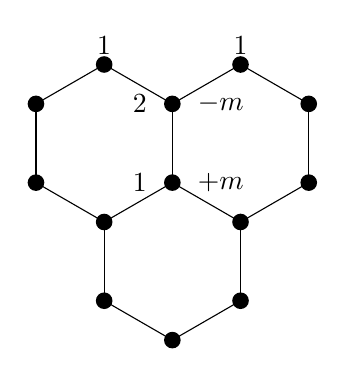
\begin{tikzpicture}
	\foreach \i in {0,1}{
		\fill (0.866+1.732*\i,1.5) circle (3pt) node[above] {1};
	}
	\foreach \i in {0,1,2}{
		\foreach \j in {0,1}{
			\fill (1.732*\i,\j) circle (3pt);
		}
	}
	\foreach \i in {0,1}{
		\foreach \j in{0,1}{
			\fill (0.866+1.732*\i,-1.5+\j) circle (3pt);
		}
	}
	\fill (1.732,-2) circle (3pt);
	\foreach \i in {0,1,2}{
		\draw (1.732*\i,0) -- (1.732*\i,1);
	}
	\foreach \i in {0,1}{
		\draw (1.732*\i,1) -- (0.866+1.732*\i,1.5);
	}
	\foreach \i in {0,1}{
		\draw (0.866+1.732*\i,1.5) -- (1.732+1.732*\i,1);
	}
	\foreach \i in {0,1}{
		\draw (1.732*\i,0) -- (0.866+1.732*\i,-0.5);
	}
	\foreach \i in {0,1}{
		\draw (0.866+1.732*\i,-0.5) -- (1.732+1.732*\i,0);
	}
	\foreach \i in {0,1}{
		\draw (0.866+1.732*\i,-1.5) -- (0.866+1.732*\i,-0.5);
	}
	\foreach \i in {0,1}{
		\draw (1.732,-2) -- (0.866+1.732*\i,-1.5);
	}
	\node[left,xshift=-0.2cm] at (1.732,1) {2};
	\node[left,xshift=-0.2cm] at (1.732,0) {1};
	\node[right,xshift=0.2cm] at (1.732,1) {$-m$};
	\node[right,xshift=0.2cm] at (1.732,0) {$+m$};
\end{tikzpicture}
\end{center}
This adds the following term to the Hamiltonian
\begin{equation}
H'(\vec{R})=m\sum_{R}\big(\ketbra*{\vec{R},1}{\vec{R},1}-\ketbra*{\vec{R},2}{\vec{R},2}\big)
\end{equation}
Upon Fourier transformation
\begin{equation}
\begin{aligned}
H'(\vec{k})&=m\big(\ketbra*{\vec{k},1}{\vec{k},1}-\ketbra*{\vec{k},2}{\vec{k},2}\big)\\
&=m\sigma^{z}
\end{aligned}
\end{equation}
Thus, the Hamiltonian becomes
\begin{equation}
H_{\pm}(\vec{k})=\hbar v_{F}(\pm k_{x}\sigma^{x}+k_{y}\sigma^{y})+m\sigma^{z}
\end{equation}
This yields the dispersion relations
\begin{equation}
\varepsilon_{\pm}(\vec{k})=\pm\sqrt{\hbar^{2}v_{F}^{2}k^{2}+m^{2}}
\end{equation}
which resembles that of massive relativistic fermions
\begin{center}
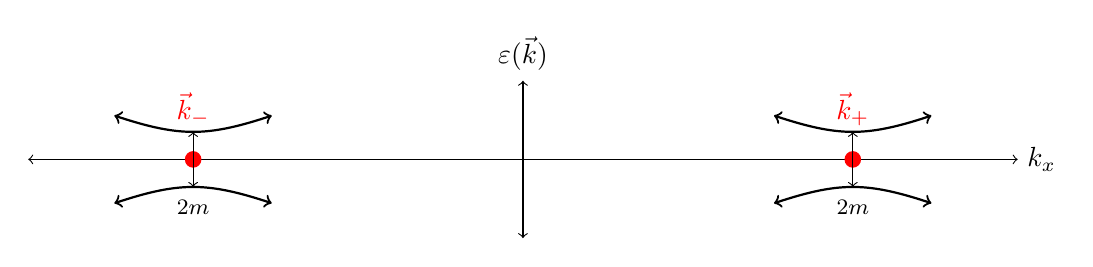
\begin{tikzpicture}
	\draw[<->] (-2*pi,0) -- (2*pi,0) node[right] {$k_{x}$};
	\draw[<->] (0,-1) -- (0,1) node[above] {$\varepsilon(\vec{k})$};
	\draw[thick,<->,domain=-5.189:-3.189,samples=200] plot (\x, {0.5*sqrt(3/4*(\x+4.189)^2+0.49)});
	\draw[thick,<->,domain=-5.189:-3.189,samples=200] plot (\x, {-0.5*sqrt(3/4*(\x+4.189)^2+0.49)});
	\draw[thick,<->,domain=3.189:5.189,samples=200] plot (\x, {0.5*sqrt(3/4*(\x-4.189)^2+0.49)});
	\draw[thick,<->,domain=3.189:5.189,samples=200] plot (\x, {-0.5*sqrt(3/4*(\x-4.189)^2+0.49)});
	\fill[red] (-4*pi/3,0) circle (3pt) node[above,yshift=0.3cm] {$\vec{k}_{-}$};
	\fill[red] (4*pi/3,0) circle (3pt) node[above,yshift=0.3cm] {$\vec{k}_{+}$};
	\draw[<->] (-4.189,-0.35) -- node[below,yshift=-0.4cm,font=\footnotesize] {$2m$} (-4.189,0.35);
	\draw[<->] (4.189,-0.35) -- node[below,yshift=-0.4cm,font=\footnotesize] {$2m$} (4.189,0.35);
\end{tikzpicture}
\end{center}

With this ``mass" term, graphene now appears as a ``regular" insulator. 
\begin{center}
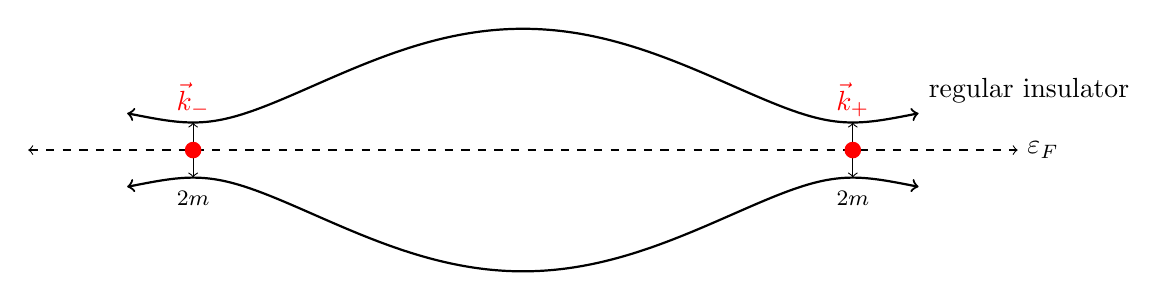
\begin{tikzpicture}
	\draw[dashed,<->] (-2*pi,0) -- (2*pi,0) node[right] {$\varepsilon_{F}$};
	\draw[thick,<->,domain=-1.6*pi:1.6*pi,samples=200] plot (\x, {0.5*sqrt((1+2*cos(deg(\x/2)))^2+0.49)}) node[above right] {regular insulator};
	\draw[thick,<->,domain=-1.6*pi:1.6*pi,samples=200] plot (\x,{-0.5*sqrt((1+2*cos(deg(\x/2)))^2+0.49)});
	\draw[<->] (-4.189,-0.35) -- node[below,yshift=-0.4cm,font=\footnotesize] {$2m$} (-4.189,0.35);
	\draw[<->] (4.189,-0.35) -- node[below,yshift=-0.4cm,font=\footnotesize] {$2m$} (4.189,0.35);
	\fill[red] (-4*pi/3,0) circle (3pt) node[above,yshift=0.3cm] {$\vec{k}_{-}$};
	\fill[red] (4*pi/3,0) circle (3pt) node[above,yshift=0.3cm] {$\vec{k}_{+}$};
\end{tikzpicture}
\end{center}
\begin{figure}[H]
	\centering
	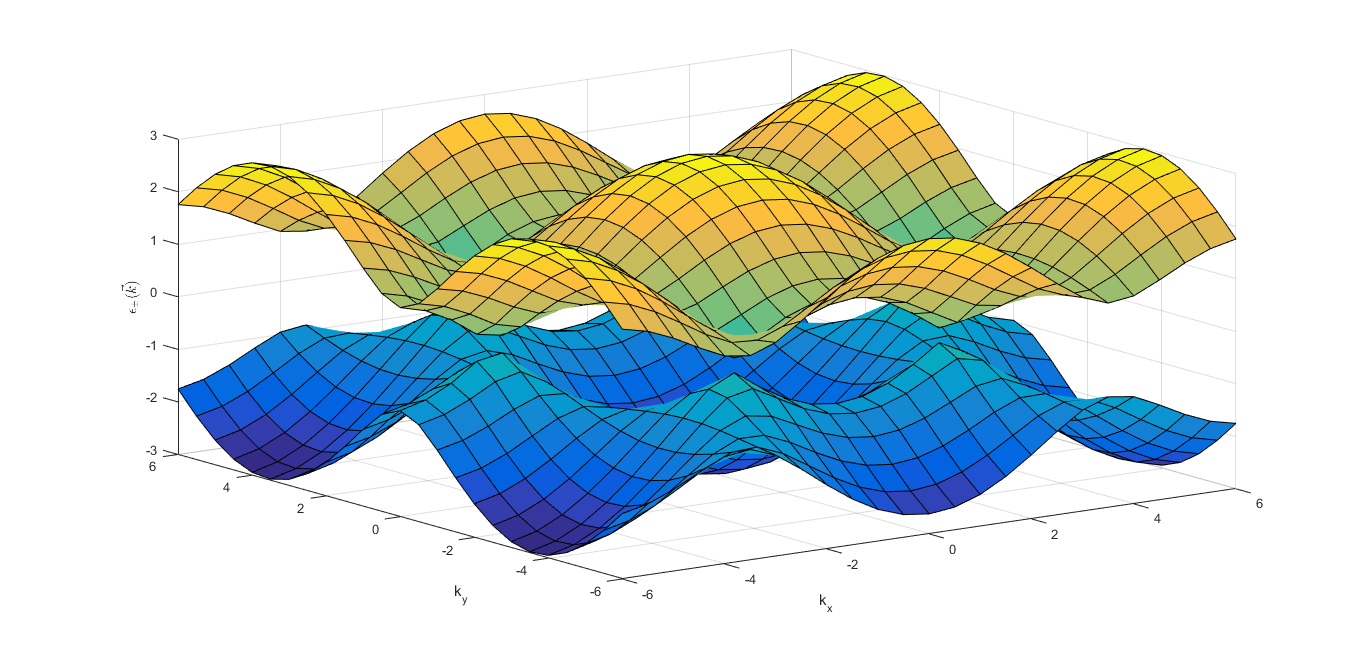
\includegraphics[width=\textwidth]{Images/2/graphene_band.png}
	\caption{Energy bands of graphene with mass term}
\end{figure}
\begin{figure}[H]
	\centering
	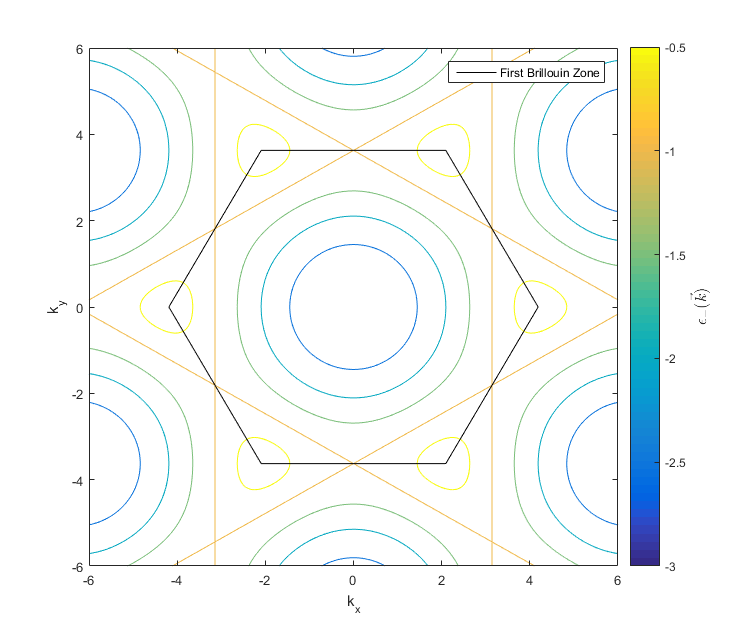
\includegraphics[width=0.7\textwidth]{Images/2/graphene_BZ.png}
	\caption{Lower energy band in first Brillouin zone of graphene with mass term}
\end{figure}
Clean graphene ($m=0$) is thus a semimetal due to inversion symmetry, but becomes an insulator when $m>0$. Returning back to the $m=0$ case
\begin{equation}
H_{\pm}(\vec{k})=\hbar v_{F}(\pm k_{x}\sigma^{x}+k_{y}\sigma^{y})
\end{equation}
The ``$\pm$" can be thought of as a two-component degree of freedom, which can be thought of as a pseudospin $\tau$ describing the $k_{+}$ or $k_{-}$ band-touching points.
\begin{equation}
\begin{aligned}
\tau^{x}&=\ketbra{+}{-}+\ketbra{-}{+}\\
\tau^{y}&=-i(\ketbra{+}{-}-\ketbra{-}{+})\\
\tau^{z}&=\ketbra{+}{+}-\ketbra{-}{-}
\end{aligned}
\end{equation}
Thus, $H(\vec{k})$ can be written as a single matrix
\begin{equation}
H(\vec{k})=\hbar v_{F}(k_{x}\tau^{z}\sigma^{x}+k_{y}\sigma^{y})+m\sigma^{z}
\end{equation}
including the ``mass" term.

\subsection{Spin-Orbit Interactions}
Let us analyze the symmetryies of $H(\vec{k})$. We shall set $m=0$. The Hamiltonian must be invariant under both time-reversal (as there is no magnetization) and inversion symmetry (i.e. parity symmetry). Thus
\begin{equation}
\Pi^{\dagger}H(\vec{k})\Pi=H(-\vec{k})\qquad\trm{and}\qquad\Theta H(\vec{k})\Theta^{-1}=H(-\vec{k})
\end{equation}
where $\Pi$ is the parity operator and $\Theta$ is the time-reversal operator.\\

Since $\tau^{z}$ refers to the two band-touching points, which are coordinates in momentum space, $\tau^{z}$ changes sign under both symmetries.
\begin{equation}
\Pi^{\dagger}\tau^{z}\Pi=-\tau^{z}\qquad\trm{and}\qquad\Theta\tau^{z}\Theta^{-1}=-\tau^{z}
\end{equation}

Furthermore, $k_{x,y,z}$ represent momentum and are thus odd under these symmetries
\begin{equation}
\Pi^{\dagger}k_{x,y,z}\Pi=-k_{x,y,z}\qquad\trm{and}\qquad\Theta k_{x,y,z}\Theta^{-1}=-k_{x,y,z}
\end{equation}

Thus, to keep $H(\vec{k})$ even under these symmetries
\begin{equation}
\begin{aligned}
\Pi^{\dagger}\sigma^{x}\Pi&=\Theta\sigma^{x}\Theta^{-1}=\sigma^{x}\\
\Pi^{\dagger}\sigma^{y}\Pi&=\Theta\sigma^{y}\Theta^{-1}=-\sigma^{y}
\end{aligned}
\end{equation}
This is intuitive as $\sigma^{x}$ and $\sigma^{y}$ refer to the spatial location of atoms 1 and 2 oriented in the $y$-direction. Based off the equations above, this implies that $\Pi=\sigma^{z}$. Thus, including the ``mass" term is prohibited as it breaks inversion symmetry. Namely
\begin{equation}
\Pi^{\dagger}\sigma^{z}\Pi=-\sigma^{z}\qquad\trm{and}\qquad\Theta\sigma^{z}\Theta^{-1}=\sigma^{z}
\end{equation}
This is also intuitive since $m\sigma^{z}$ adds a spatial discrepancy between atoms 1 and 2.\\

What other $k$-independent terms can be added to $H(\vec{k})$ that do not violate these symmetries, such that there is still a gap in graphene? In reality, the violation of symmetry is an artifact of our nearest-neighbour model. If the next-nearest neighbours are included, it is possible to recover these symmetries. This was realized by Charles Kane.\\

Note that under inversion
\begin{equation}
\Pi^{\dagger}\tau^{z}\sigma^{z}\Pi=\tau^{z}\sigma^{z}
\end{equation}
However, under time-reversal
\begin{equation}
\Theta\tau^{z}\sigma^{z}\Theta^{-1}=-\tau^{z}\sigma^{z}
\end{equation}

We resolve this by accounting for the real spin (not pseudospins) of electrons $S$. Spin $S$ is parity even and time-reversal odd. Thus
\begin{equation}
\Pi^{\dagger}S\Pi=S\qquad\trm{and}\qquad\Theta S\Theta^{-1}=-S
\end{equation}
where
\begin{equation}
\begin{aligned}
S^{x}&=\ketbra{\up}{\dn}+\ketbra{\dn}{\up}\\
S^{y}&=-i\big(\ketbra{\up}{\dn}-\ketbra{\dn}{\up}\big)\\
S^{z}&=\ketbra{\up}{\up}-\ketbra{\dn}{\dn}
\end{aligned}
\end{equation}

Thus, the term $\sigma^{z}\tau^{z}S^{z}$ satisfies these symmetries
\begin{equation}
\Pi^{\dagger}\sigma^{z}\tau^{z}S^{z}\Pi=\Theta\sigma^{z}\tau^{z}S^{z}\Theta^{-1}=\sigma^{z}\tau^{z}S^{z}
\end{equation}

Thus, the real Hamiltonian of graphene is
\begin{equation}
H(\vec{k})=\hbar v_{F}(k_{x}\tau^{z}\sigma^{x}+k_{y}\sigma^{y})+\Delta_{\trm{SO}}\sigma^{z}\tau^{z}S^{z}
\end{equation}
$\Delta_{\trm{SO}}$ refers to \ul{spin-orbit interactions}. This term was discovered by Kane and Mele (2005) and their paper gave rise to the field of topological insulators.\\

The spin-orbit interaction is a relativistic effect. An electron moves in the electric field of ionized atoms in the crystal lattice. The electric field $\vec{E}$ in the rest frame of an electron will be transferred to a magnetic field
\begin{equation}
\vec{B}=\frac{\vec{v}}{c}\times\vec{E}=\frac{\vec{p}}{mc}\times\vec{E}
\end{equation}
This electric field is felt as a magnetic field by the electron in its rest frame which acts on electron spin (i.e. $\vec{B}\cdot\vec{S}=\frac{\vec{p}\times\vec{E}}{mc}\cdot\vec{S}$). This couples spin with momentum in a spin-orbit interaction. This is encapsulated as $\tau^{z}\sigma^{z}$ couples with $S^{z}$. Recall that $\tau^{z}$ refers to momentum (namely $\vec{k}_{+}$ and $\vec{k}_{-}$).\\

Within the tight-binding approximation of graphene, the $\Delta_{\trm{SO}}$ term arises from second-nearest neighbour spin-dependent hopping.
\begin{center}
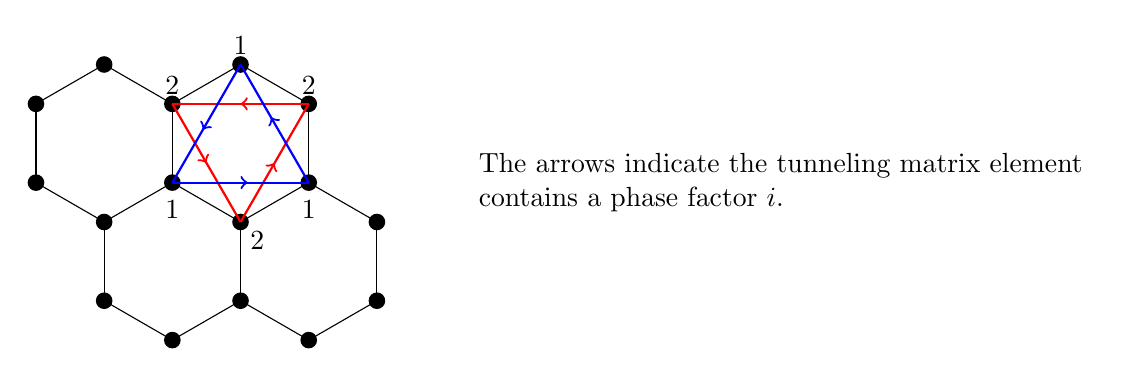
\begin{tikzpicture}
	\foreach \i in {0,1}{
		\fill (0.866+1.732*\i,1.5) circle (3pt);
	}
	\foreach \i in {0,1,2}{
		\foreach \j in {0,1}{
			\fill (1.732*\i,\j) circle (3pt);
		}
	}
	\foreach \i in {0,1,2}{
		\foreach \j in{0,1}{
			\fill (0.866+1.732*\i,-1.5+\j) circle (3pt);
		}
	}
	\foreach \i in {1,2}{
		\fill (1.732*\i,-2) circle (3pt);
	}
	\foreach \i in {0,1,2}{
		\draw (1.732*\i,0) -- (1.732*\i,1);
	}
	\foreach \i in {0,1}{
		\draw (1.732*\i,1) -- (0.866+1.732*\i,1.5);
	}
	\foreach \i in {0,1}{
		\draw (0.866+1.732*\i,1.5) -- (1.732+1.732*\i,1);
	}
	\foreach \i in {0,1,2}{
		\draw (1.732*\i,0) -- (0.866+1.732*\i,-0.5);
	}
	\foreach \i in {0,1}{
		\draw (0.866+1.732*\i,-0.5) -- (1.732+1.732*\i,0);
	}
	\foreach \i in {0,1,2}{
		\draw (0.866+1.732*\i,-1.5) -- (0.866+1.732*\i,-0.5);
	}
	\foreach \i in {0,1}{
		\draw (1.732,-2) -- (0.866+1.732*\i,-1.5);
	}
	\foreach \i in {0,1}{
		\draw (3.464,-2) -- (2.598+1.732*\i,-1.5);
	}
	\foreach \i in {0,1}{
		\node[above] at (1.732+1.732*\i,1) {2};
	}
	\foreach \i in {0,1}{
		\node[below,yshift=-0.1cm] at (1.732+1.732*\i,0) {1};
	}
	\node[above] at (2.598,1.5) {1};
	\node[below right] at (2.598,-0.5) {2};
	
	\draw[red,thick,->-=0.5] (1.732,1) -- (2.598,-0.5);
	\draw[red,thick,->-=0.5] (2.598,-0.5) -- (3.464,1);
	\draw[red,thick,->-=0.5] (3.464,1) -- (1.732,1);
	\draw[blue,thick,-<-=0.5] (1.732,0) -- (2.598,1.5);
	\draw[blue,thick,-<-=0.5] (2.598,1.5) -- (3.464,0);
	\draw[blue,thick,-<-=0.5] (3.464,0) -- (1.732,0);
	\node[anchor=north west,right,text width=8cm] at (5.5,0)
		{The arrows indicate the tunneling matrix element contains a phase factor $i$.};
\end{tikzpicture}
\end{center}
\begin{equation}
\begin{aligned}
H'=-it'\big(&\ketbra*{\vec{R}+\vec{a}_{1}-\vec{a}_{2},1}{\vec{R},1}+\ketbra*{\vec{R}+\vec{a}_{1},1}{\vec{R}+\vec{a}_{1}-\vec{a}_{2},1}+\ketbra*{\vec{R},1}{\vec{R}+\vec{a}_{1},1}\\
&-\ketbra*{\vec{R},2}{\vec{R}+\vec{a}_{1}-\vec{a}_{2},2}-\ketbra*{\vec{R}+\vec{a}_{1}-\vec{a}_{@},2}{\vec{R}+\vec{a}_{1},2}-\ketbra*{\vec{R}+\vec{a}_{1},2}{\vec{R},2}\big)+\trm{h.c.}
\end{aligned}
\end{equation}
The negative sign occurs over due to the opposing directions of the tunneling amplitudes. After performing a Fourier transform and evaluating the resulting $\vec{k}$-dependent coefficient at $\vec{k}_{\pm}$, one finds
\begin{equation}
\Delta_{\trm{SO}}=3\sqrt{3}t'
\end{equation}
Refer to assignment 3 for more details on the derivation.\\

In order to study the effects of the $\Delta_{\trm{SO}}$ term, let us add back the $m\sigma^{z}$ term in the Hamiltonian.
\begin{equation}
H(\vec{k})=\hbar v_{F}(k_{x}\tau^{z}\sigma^{x}+k_{y}\sigma^{y})+\Delta_{\trm{SO}}\tau^{z}\sigma^{z}S^{z}+m\sigma^{z}
\end{equation}

Consider spin up electrons ($S^{z}=1$)
\begin{equation}
\begin{aligned}
H_{+}(\vec{k})&=\hbar v_{F}(k_{x}\sigma^{x}+k_{y}\sigma^{y})+(m+\Delta_{\trm{SO}})\sigma^{z}\\
H_{-}(\vec{k})&=\hbar v_{F}(-k_{x}\sigma^{x}+k_{y}\sigma^{y})+(m-\Delta_{\trm{SO}})\sigma^{z}
\end{aligned}
\end{equation}

The eigenvalues for the Hamiltonians are
\begin{equation}
\begin{aligned}
\varepsilon_{+}(\vec{k})&=\pm\sqrt{\hbar^{2}v_{F}^{2}k^{2}+(m+\Delta_{\trm{SO}})^{2}}\\
\varepsilon_{-}(\vec{k})&=\pm\sqrt{\hbar^{2}v_{F}^{2}k^{2}+(m-\Delta_{\trm{SO}})^{2}}
\end{aligned}
\end{equation}

In the limit of large $m\gg\Delta_{\trm{SO}}$, all the electrons will localize to atoms of type 2 due to lower energy costs. Even with tunneling between atoms of type 2, the localization of electrons prevents it by the Pauli exclusion principle. Thus, we obtain an insulator. Moreover, this is a trivial (non-topological) insulator, as increasing $m$ to infinity simply corresponds to a gas of disconnected carbon atoms (i.e. an atomic insulator).
\begin{center}
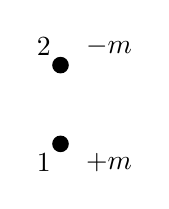
\begin{tikzpicture}
	\fill (0,1) circle (3pt) node[above left] {2} node[above right,xshift=0.2cm] {$-m$};
	\fill (0,0) circle (3pt) node[below left] {1} node[below right,xshift=0.2cm] {$+m$};
\end{tikzpicture}
\end{center}

Suppose we decrease $m$, while still letting it be positive.
\begin{center}
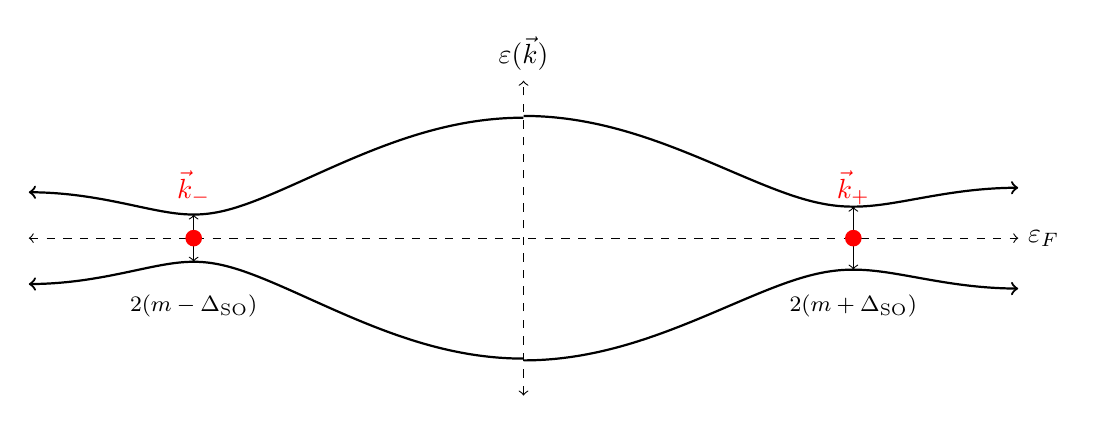
\begin{tikzpicture}
	\draw[dashed,<->] (-2*pi,0) -- (2*pi,0) node[right] {$\varepsilon_{F}$};
	\draw[dashed,<->] (0,-2) -- (0,2) node[above] {$\varepsilon(\vec{k})$};
	\draw[thick,<-,domain=-2*pi:0,samples=200] plot (\x, {0.5*sqrt((1+2*cos(deg(\x/2)))^2+(0.7-0.1)^2)});
	\draw[thick,<-,domain=-2*pi:0,samples=200] plot (\x,{-0.5*sqrt((1+2*cos(deg(\x/2)))^2+(0.7-0.1)^2)});
	\draw[thick,->,domain=0:2*pi,samples=200] plot (\x, {0.5*sqrt((1+2*cos(deg(\x/2)))^2+(0.7+0.1)^2)});
	\draw[thick,->,domain=0:2*pi,samples=200] plot (\x,{-0.5*sqrt((1+2*cos(deg(\x/2)))^2+(0.7+0.1)^2)});
	\draw[<->] (-4.189,-0.3) -- node[below,yshift=-0.6cm,font=\footnotesize] {$2(m-\Delta_{\trm{SO}})$} (-4.189,0.3);
	\draw[<->] (4.189,-0.4) -- node[below,yshift=-0.6cm,font=\footnotesize] {$2(m+\Delta_{\trm{SO}})$} (4.189,0.4);
	\fill[red] (-4*pi/3,0) circle (3pt) node[above,yshift=0.3cm] {$\vec{k}_{-}$};
	\fill[red] (4*pi/3,0) circle (3pt) node[above,yshift=0.3cm] {$\vec{k}_{+}$};
\end{tikzpicture}
\end{center}
The ``mass" at the $\vec{k}_{+}$ remains positive, but the ``mass" at the $\vec{k}_{-}$ band-touching point vanishes and changes sign when $m=\Delta_{\trm{SO}}$. The gap is $2\abs{m-\Delta_{\trm{SO}}}$ and closes at this value of $m$. This signifies a transition between two different kinds of insulators.
\begin{itemize}
\item $m>\Delta_{\trm{SO}}$: Trivial insulator
\item $m=\Delta_{\trm{SO}}$: Transition point / semimetal
\item $m>\Delta_{\trm{SO}}$: Topological insulator
\end{itemize}

Recall $H(\vec{k})=\vec{d}(\vec{k})\cdot\vec{\sigma}$. Let us analyze $\hat{d}(\vec{k})=\frac{\vec{d}(\vec{k})}{\abs*{\vec{d}(\vec{k})}}$. $\hat{d}(\vec{k})$ can be thought of as a map from the first Brillouin zone to the surface of a unit sphere. This will allow us to interpret the topological differences between ordinary and topological insulators.\\

Near the band-touching points
\begin{equation}
\begin{aligned}
\hat{d}(\vec{k}_{+})&=\frac{1}{\sqrt{\hbar^{2}v_{F}^{2}k^{2}+(m+\Delta_{\trm{SO}})^{2}}}(\hbar v_{F}k_{x},\,\hbar v_{F}k_{y},\,m+\Delta_{\trm{SO}})\\
\hat{d}(\vec{k}_{-})&=\frac{1}{\sqrt{\hbar^{2}v_{F}^{2}k^{2}+(m-\Delta_{\trm{SO}})^{2}}}(-\hbar v_{F}k_{x},\,\hbar v_{F}k_{y},\,m-\Delta_{\trm{SO}})
\end{aligned}
\end{equation}
When $m>\Delta_{\trm{SO}}$, the $z$-component of both $\hat{d}(\vec{k}_{+})$ and $\hat{d}(\vec{k}_{-})$ are always positive. Thus, $\hat{d}(\vec{k})$ only covers the upper hemisphere of the unit sphere as $\vec{k}$ covers the whole Brillouin zone. When $m<\Delta_{\trm{SO}}$, the $z$-component of $\hat{d}(\vec{k}_{-})$ is always negative. As $\vec{k}$ covers the whole Brillouin zone, $\hat{d}(\vec{k})$ covers the entire unit sphere.
\medskip
\begin{center}
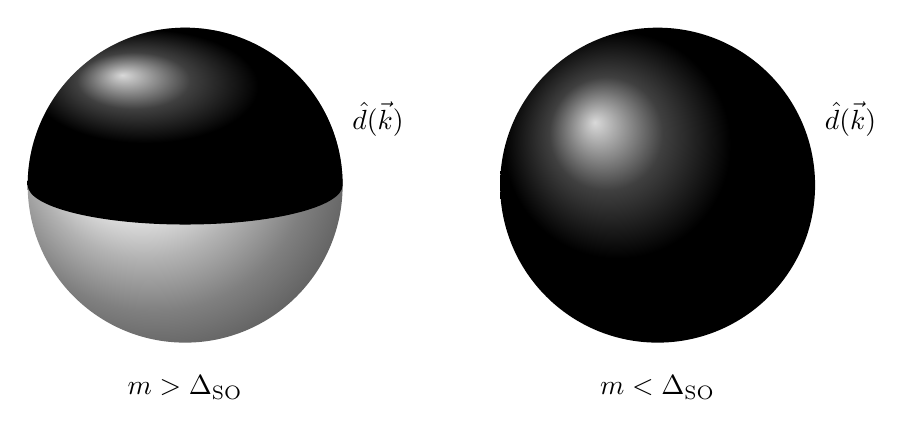
\begin{tikzpicture}
	\shade[ball color=white] (2,0) circle (2cm) node[below,yshift=-2.3cm] {$m>\Delta_{\trm{SO}}$} node[above right,xshift=2cm,yshift=0.5cm] {$\hat{d}(\vec{k})$}; 
	\fill[color=black] (0,0) arc (180:360:2cm and 0.5cm);
	\shade[ball color=black] (0,0) arc (180:0:2cm) ;
	\shade[ball color=black] (8,0) circle (2cm) node[below,yshift=-2.3cm] {$m<\Delta_{\trm{SO}}$} node[above right,xshift=2cm,yshift=0.5cm] {$\hat{d}(\vec{k})$};
\end{tikzpicture}
\end{center}
Given this observation, we can define a \ul{topological invariant} that characterizes the differences in these two topologically distinct situations corresponding to the two types of insulators. The quantity is $\eta\in\{0,1\}$ and is defined as
\begin{equation}
\eta=\frac{1}{4\pi}\int_{\trm{BZ}}\hat{d}\cdot(\partial_{k_{x}}\hat{d}\times\partial_{k_{y}}\hat{d})\dd[2]{k}=\begin{cases}
1, & \trm{if topological}\\
0, & \trm{if trivial}
\end{cases}
\end{equation}
where $\int_{\trm{BZ}}$ indicates an integration over the entire Brillouin zone. The quantity $\eta$ is related to the \ul{Chern number}. In this particular case
\begin{equation}
\eta=\begin{cases}
1, & m<\Delta_{\trm{SO}}\\
0, & m>\Delta_{\trm{SO}}
\end{cases}
\end{equation}

\subsection{Topological/Non-Topological Interfaces}
Just as in polyacetylene, the topological distinction gives rise to edge states at the interface between topological and ordinary insulators. To describe this, let us consider $H(\vec{k})$.
\begin{equation}
H_{-}(\vec{k})=\hbar v_{F}(-k_{x}\sigma^{x}+k_{y}\sigma^{y})+(m-\Delta_{\trm{SO}})\sigma^{z}
\end{equation}
The coefficient in front of $\sigma^{z}$ differs in sign depending on the type of insulator. Assume the material transitions from a topological insulator to an ordinary insulator by letting $m(x)$ denote this coefficient as it varies along $x$. Note that this discussion implies that $\tau^{z}$ and $S^{z}$ must be of opposite signs, otherwise the interface would be between two trivial insulators.
\begin{equation}
m(x)=m-\Delta_{\trm{SO}}
\end{equation}
Since $k_{x}$ no longer corresponds with plane wave solutions to the Schr\"{o}dinger equation, replace $k_{x}$ with its representation in position space.
\begin{equation}
k_{x}\rightarrow-i\pdv{x}
\end{equation}

Thus
\begin{equation}
H_{-}(k_{y})=i\hbar v_{F}\pdv{x}\sigma^{x}+\hbar v_{F}k_{y}\sigma^{y}+m(x)\sigma^{z}
\end{equation}

Let us start with $k_{y}=0$ and find the zero energy eigenstate solution for the Schr\"{o}dinger equation. We let $m(x\rightarrow-\infty)$ be negative, corresponding to a topological insulator and $m(x\rightarrow\infty)$ be positive, corresponding to a trivial insulator. This is analogous to what we did for polyacetylene. Thus, we look for solutions of the form
\begin{equation}
\Psi(x)=e^{f(x)}\sigma^{x}\ket{z}
\end{equation}
where as before
\begin{equation}
\ket{z}=z_{1}\ket{1}+z_{2}\ket{2}
\end{equation}
Recall that $\sigma^{z}\sigma^{x}=i\sigma^{y}$. Thus
\begin{equation}
\begin{aligned}
H_{-}(k_{y}=0)\Psi(x)&=0\\
-\left[i\hbar v_{F}\dv{f}{x}+im(x)\sigma^{y}\right]e^{f(x)}\ket{z}&=0\\
\left[\dv{f}{x}+\frac{m(x)}{\hbar v_{F}}\sigma^{y}\right]&=0
\end{aligned}
\end{equation}
Taking $\ket{z}$ to be an eigenstate of $\sigma^{y}$ with eigenstate 1
\begin{equation}
\sigma^{y}\ket{z}=\ket{z}
\end{equation}
Thus
\begin{equation}
\begin{aligned}
\dv{f}{x}&=-\frac{1}{\hbar v_{F}}m(x)\\
f(x)&=-\frac{1}{\hbar v_{F}}\int_{0}^{x}m(x')\dd{x'}
\end{aligned}
\end{equation}
and therefore
\begin{equation}
\Psi(x)=e^{-\frac{1}{\hbar v_{F}}\int_{0}^{x}m(x')\dd{x'}}\sigma^{x}\ket{z}
\end{equation}

\begin{center}
\begin{tikzpicture}
	\draw[<->] (-4,0) -- (4,0) node[right] {$x$};
	\draw[<->] (0,2.5) node[above] {$\Psi(x)$} -- (0,-0.5);
	\draw[thick,domain=-4:4,samples=200,red,<->] plot (\x, {2*e^(-(\x)^2)+0.1});
\end{tikzpicture}
\end{center}

Additionally
\begin{equation}
\sigma^{y}\sigma^{x}\ket{z}=-\sigma^{x}\sigma^{y}\ket{z}=-\sigma^{x}\ket{z}
\end{equation}
Thus, $\sigma^{x}\ket{z}$ is an eigenstate of $\sigma^{y}$ with eigenvalue -1 and the solution is of the form
\begin{equation}
\Psi(x)=e^{-\frac{1}{\hbar v_{F}}\int_{0}^{x}m(x')\dd{x'}}\ket{\sigma^{y}=-1}
\end{equation}
This is known as the Jackiw-Rebbi solution.\\

Consider a non-zero $k_{y}$
\begin{equation}
\begin{aligned}
H_{-}(k_{y})\Psi(x)&=\hbar v_{F}k_{y}\sigma^{y}e^{-\frac{1}{\hbar v_{F}}\int_{0}^{x}m(x')\dd{x'}}\ket{\sigma^{y}=-1}\\
&\quad\explain\trm{ Since }H_{-}(k_{y}=0)\Psi(x)=0\\
&=-\hbar v_{F}k_{y}e^{-\frac{1}{\hbar v_{F}}\int_{0}^{x}m(x')\dd{x'}}\ket{\sigma^{y}=-1}\\
&=-\hbar v_{F}k_{y}\Psi(x)
\end{aligned}
\end{equation}

Thus, $\Psi(x)$ is an eigenstate of $H_{-}(k_{y})$ with eigenvalue $-\hbar v_{F}k_{y}$. Plotting the dispersion relation
\begin{center}
\begin{tikzpicture}
	\draw[<->] (-4,0) -- (4,0) node[right] {$k_{y}$};
	\draw[<->] (0,4) node[above] {$\varepsilon(k_{y})$} -- (0,-4);
	\draw[<->,ultra thick] (-1,4) -- (1,-4);
	\draw[->,shorten >=1mm] (2,-2) node[right] {$\varepsilon(k_{y})=-\hbar v_{F}k_{y}$} -- (0.5,-2);
\end{tikzpicture}
\end{center}
This kind of edge state is called a \ul{chiral edge state}. The dispersion is called a \ul{chiral dispersion}. This dispersion resembles that of a left-handed Weyl fermion in 1D.\\

Recall that the formula for \ul{group velocity} is
\begin{equation}
\vec{v}=\frac{1}{\hbar}\vec{\nabla}_{k}\varepsilon(\vec{k})
\end{equation}
This can be seen knowing that $\vec{v}=\vec{\nabla}_{k}\omega(\vec{k})$ and $\varepsilon(\vec{k})=\hbar\omega(\vec{k})$. Thus, the group velocity is $\vec{v}=-v_{F}\hat{y}$ and all electrons in this state move in one direction.
\begin{center}
\begin{tikzpicture}
	\draw (0,2) -- (0,-2);
	\draw[->,red,thick] (-0.3,1.5) -- (-0.3,-1.5);
	\draw[<-,shorten >=1mm] (-0.5,-1) -- (-1,-2) node[left] {chiral pseudospin edge state};
	\node at (-3,0) {Topological};
	\node at (3,0) {Trivial};
	\draw[->] (0.5,1) -- (0.5,2) node[above] {$\hat{y}$};
	\draw[->] (0.5,1) -- (1.5,1) node[right] {$\hat{x}$};	
\end{tikzpicture}
\end{center}
This was done for $S^{z}=1$ spin-up electrons. The same analysis can be done for $S^{z}=-1$ spin-down electrons (where $\ket{z}$ is instead an eigenstate of $\sigma^{y}$ with eigenvalue 1). This gives $\varepsilon(k_{y})=\hbar v_{F}k_{y}$ (i.e. they all move in the opposite direction). $\varepsilon(k_{y})=\pm\hbar v_{F}k_{y}$ is a band dispersion for a one-dimensional ``wire" located at the interface. Note this differs for a real 1D wire found earlier with $\varepsilon(k_{y})=-2t\cos(k_{y}a)$.
\begin{center}
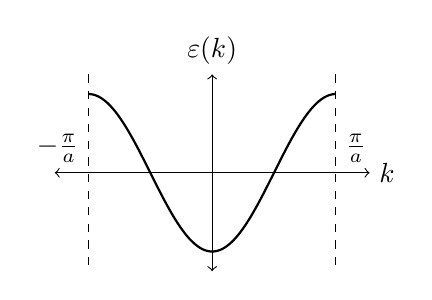
\begin{tikzpicture}[scale=0.5]
	\draw[<->] (-4,0) -- (4,0) node[right] {$k$};
	\draw[<->] (0,-2.5) -- (0,2.5) node[above] {$\varepsilon(k)$};
	\draw[thick,domain=-pi:pi,samples=200] plot (\x, {-2*cos(deg(\x)});
	\draw[dashed] (-pi,2.5) -- node[above left] {$-\frac{\pi}{a}$} (-pi,-2.5); 
	\draw[dashed] (pi,2.5) -- node[above right] {$\frac{\pi}{a}$} (pi,-2.5);
\end{tikzpicture}
\end{center}

\subsection{Quantum Spin Hall Effect}
For a finite 2D sample, spin up electrons orbit along the interface in one direction while the spin down electrons orbit in the opposite direction. This is the \ul{quantum spin Hall effect}.

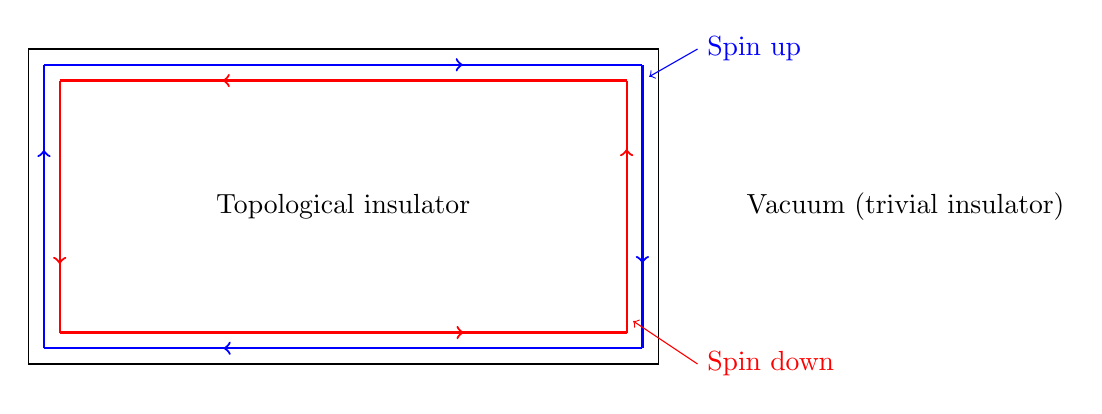
\begin{tikzpicture}
	\draw (-4,2) rectangle (4,-2);
	\coordinate (tl) at (-4,2);
	\coordinate (tr) at (4,2);
	\coordinate (bl) at (-4,-2);
	\coordinate (br) at (4,-2);
	\draw[->-=0.7,blue,thick] ([shift={(0.2,-0.2)}]tl) -- ([shift={(-0.2,-0.2)}]tr);
	\draw[->-=0.7,blue,thick] ([shift={(-0.2,-0.2)}]tr) -- ([shift={(-0.2,0.2)}]br);
	\draw[->-=0.7,blue,thick] ([shift={(-0.2,0.2)}]br) -- ([shift={(0.2,0.2)}]bl);
	\draw[->-=0.7,blue,thick] ([shift={(0.2,0.2)}]bl) -- ([shift={(0.2,-0.2)}]tl);
	\draw[-<-=0.3,red,thick] ([shift={(0.4,-0.4)}]tl) -- ([shift={(-0.4,-0.4)}]tr);
	\draw[-<-=0.3,red,thick] ([shift={(-0.4,-0.4)}]tr) -- ([shift={(-0.4,0.4)}]br);
	\draw[-<-=0.3,red,thick] ([shift={(-0.4,0.4)}]br) -- ([shift={(0.4,0.4)}]bl);
	\draw[-<-=0.3,red,thick] ([shift={(0.4,0.4)}]bl) -- ([shift={(0.4,-0.4)}]tl);
	\node[right] at (5,0) {Vacuum (trivial insulator)};
	\node at (0,0) {Topological insulator};
	\draw[<-,shorten <=1mm,blue] (3.8,1.6) -- (4.5,2) node[right] {Spin up};
	\draw[<-,shorten <=1mm,red] (3.6,-1.4) -- (4.5,-2) node[right] {Spin down};
\end{tikzpicture}
There are two dispersion relations given by
\begin{center}
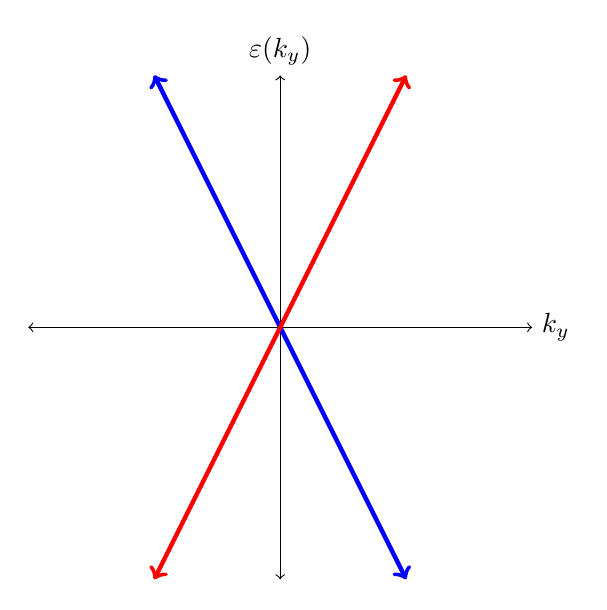
\begin{tikzpicture}[scale=0.8]
	\draw[<->] (-4,0) -- (4,0) node[right] {$k_{y}$};
	\draw[<->] (0,-4) -- (0,4) node[above] {$\varepsilon(k_{y})$};
	\draw[<->,ultra thick,blue] (-2,4) -- (2,-4);
	\draw[<->,ultra thick,red] (-2,-4) -- (2,4);
\end{tikzpicture}
\end{center}
Using an external potential $V_{y}$, electrons pool on one side in the $y$-direction.
\begin{center}
\begin{tikzpicture}
	\draw (-3,2) rectangle (3,-2);
	\draw (2.8,2) -- (2.8,2.5) -- (4.5,2.5) -- (4.5,-2.5) -- (2.8,-2.5) -- (2.8,-2);
	\draw[fill=white] (4.5,0) circle (25pt) node[font=\large] {$V_{y}$};
	\draw[->] (3.2,-1) -- (3.2,1);
	\foreach \i in {0,...,10}{
		\node[red,thick] at (-2.5+0.5*\i,1.5) {$+$};
		\node[red,thick] at (-2.5+0.5*\i,-1.5) {$-$};
	}
	\draw[->] (6,0) -- (6,1) node[above] {$\hat{y}$};
	\draw[->] (6,0) -- (7,0) node[right] {$\hat{x}$};	
\end{tikzpicture}
\end{center}
Consider a sample with two edges. In the absence of an external voltage across the $y$-direction, the net current is zero as the two edges cancel each other. However, after applying a voltage drop between the upper and lower edge, the occupation of electrons will differ between the sides and a net current flows in the $x$-direction due to the quantum spin Hall effect. Since $P=IV$ but the current flows orthogonally to the applied voltage, there is no dissipation of energy. This is the \ul{Hall effect}, where there is current flowing perpendicular to the applied voltage.

\begin{center}
\begin{tikzpicture}
	\draw (-5,2) -- (5,2);
	\draw (-5,-2) -- (5,-2);
	\draw (6,1) -- (6,2) node[above] {$\hat{y}$};
	\draw (6,1) -- (7,1) node[right] {$\hat{x}$};
	\draw[->] (-4.5,1.5) -- (4.5,1.5);
	\draw[<-] (-4.5,-1.5) -- (4.5,-1.5);
\end{tikzpicture}
\end{center}

For a wire with electrons flowing through it
\begin{center}
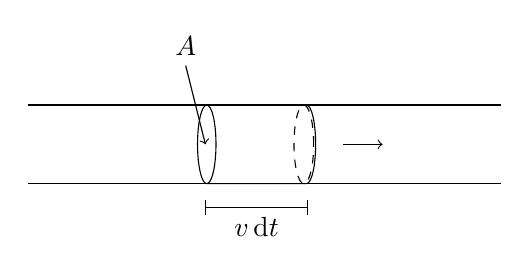
\begin{tikzpicture}
	\node[cylinder,shape border rotate=180,draw,minimum height=1.5cm,minimum width=1cm] at (0,0) {};
	\draw (-3,0.5) -- (3,0.5);
	\draw (-3,-0.5) -- (3,-0.5);
	\draw[|-|] (-0.75,-0.8) -- node[below] {$v\dd{t}$} (0.55,-0.8);
	\draw[->] (1,0) -- (1.5,0);
	\draw[dashed] (0.5,0) circle[x radius=0.125cm,y radius=0.5cm];
	\draw[<-] (-0.75,0) -- (-1,1) node[above] {$A$};
\end{tikzpicture}
\end{center}
where $I=\dv{Q}{t}$ is the current, $n$ is the electron density, and $-e$ is the charge of the electron.\\

The charge flowing through this cross-section per time $\dd{t}$ is
\begin{equation}
\begin{aligned}
\dd{Q}&=-enAv\dd{t}\\
\dv{Q}{t}&=-enAv
\end{aligned}
\end{equation}
Thus, one defines the \ul{current density} $j$
\begin{equation}
I=ja
\end{equation}
where $j=-env$. More generally
\begin{equation}
\vec{j}=-en\vec{v}
\end{equation}

\begin{center}
\begin{tikzpicture}
	\draw (-5,2) -- (5,2);
	\draw (-5,-2) -- (5,-2);
	\draw[->] (-4.5,1.5) -- (4.5,1.5);
	\draw[<-] (-4.5,-1.5) -- (4.5,-1.5);
	\node at (2.5,1) {$I_{\trm{top}}\equiv I_{R}$};
	\node at (-2.5,-1) {$I_{\trm{bottom}}\equiv I_{L}$};
\end{tikzpicture}
\end{center}

The electron density $n$ can be written as an integral over momentum space. This gives $I_{R}$ as
\begin{equation}
I_{R}=-e\int v_{F}n_{F}(\varepsilon_{k}) \frac{\dd{k_{x}}}{2\pi}
\end{equation}
Since $k=2\pi n/L$, $\dd{k_{x}}/\left(\frac{2\pi}{L}\right)$ is the volume in momentum space corresponding to a single quantum state. To obtain an area
\begin{equation}
A=\frac{V}{L}=\frac{\dd{k_{x}}}{2\pi}
\end{equation}
Correspondingly
\begin{equation}
I_{L}=e\int v_{F}n_{F}(\varepsilon_{k}) \frac{\dd{k_{x}}}{2\pi}
\end{equation}

Since $\varepsilon=\hbar v_{F}k_{x}$, $\dd{\varepsilon}=\hbar v_{F}\dd{k_{x}}$. Thus
\begin{equation}
\begin{aligned}
I_{R}&=-\frac{e}{2\pi n}\int_{-\infty}^{\varepsilon_{FR}}\dd{\varepsilon}n_{F}(\varepsilon)\\
I_{L}&=\frac{e}{2\pi n}\int_{-\infty}^{\varepsilon_{FL}}\dd{\varepsilon}n_{F}(\varepsilon)\\
\end{aligned}
\end{equation}

\begin{center}
\begin{tikzpicture}
	\draw[->] (0,0) -- (4,0) node[right] {$\varepsilon$};
	\draw[->] (0,0) -- (0,2) node[above] {$n_{F}$};
	\draw (3,1.5) -- (0,1.5) node[left] {1};
	\draw (3,1.5) -- (3,0) node[below] {$\varepsilon_{F}$};
	\fill[fill opacity=0.2] (0,0) rectangle (3,1.5);
\end{tikzpicture}
\end{center}

The net current is
\begin{equation}
\begin{aligned}
I&=I_{L}+I_{R}\\
&=-\frac{e}{2\pi n}\left(\int_{-\infty}^{\varepsilon_{FR}}\dd{\varepsilon}n_{F}(\varepsilon)-\int_{-\infty}^{\varepsilon_{FL}}\dd{\varepsilon}n_{F}(\varepsilon)\right)\\
&=-\frac{e}{h}\left(\int_{\varepsilon_{FL}}^{\varepsilon_{FR}}\dd{\varepsilon}\right)\trm{, since $n_{F}(\varepsilon)=1$ in these bounds}\\
&=-\frac{e}{h}(\varepsilon_{FR}-\varepsilon_{FL})
\end{aligned}
\end{equation}

\newpage
Moreover
\begin{center}
\begin{tikzpicture}
	\draw (-5,2) -- (5,2);
	\draw (-5,-2) -- (5,-2);
	\draw[->] (-4.5,1.5) -- (4.5,1.5);
	\draw[<-] (-4.5,-1.5) -- (4.5,-1.5);
	\draw(2,2) -- (2,2.5) -- (3,2.5) -- (3,-2.5) -- (2,-2.5) -- (2,-2);
	\draw[fill=white] (3,0) circle (25pt) node[font=\large] {$V_{y}$};
	\node[above right] at (4,2) {spin up};
	\node[right] at (5,0) {$\varepsilon_{FR}-\varepsilon_{FL}=eV_{y}$}; 
\end{tikzpicture}
\end{center}

Thus
\begin{equation}
I_{x}=-\frac{e^{2}}{h}V_{y}=\sigma_{xy}V_{y}
\end{equation}
where $\sigma_{xy}=-\frac{e^{2}}{h}$ is the \ul{Hall conductivity}. The Hall conductivity $\sigma_{xy}$ is the off-diagonal component of the conductivity tensor. The fact that $\sigma_{xy}$ is perfectly universal and depends only on fundamental constants is the quantum Hall effect.\\

However, spin up and spin down electrons move in different directions. Thus
\begin{equation}
\begin{aligned}
\sigma_{xy}^{\up}&=-\frac{e^{2}}{h}\\
\sigma_{xy}^{\dn}&=\frac{e^{2}}{h}\\
\sigma_{xy}&=\sigma_{xy}^{\up}+\sigma_{xy}^{\dn}=0
\end{aligned}
\end{equation}

Let us introduce a \ul{spin-current} with \ul{spin-hall conductivity}
\begin{equation}
\sigma_{xy}^{s}=\frac{1}{2}(\sigma_{xy}^{\up}-\sigma_{xy}^{\dn})=-\frac{e^{2}}{h}
\end{equation}
Effectively, there is an equal number of electrons moving in either direction, but each direction is biased to a spin. There is buildup of spin up electrons to the right and spin down electrons to the left. This is the analogue of \ul{spin voltage}. We see these in topological insulators such as HgTe and CdTe.

\subsection{Bravais Lattices in 3D}
Let us discuss 3D topological insulators. We will use a simplistic model called the Fu-Kane-Mele model that generalizes graphene to 3D. Note it does not represent any real material. The model involves electrons hopping on a diamond lattice. The diamond lattice has two atoms per unit cell, with the Bravais lattice being face-centred cubic.\\

Recall 3D Bravais lattices. There are 14 different types but we shall only discuss the cubic family.
\begin{enumerate}
\item Simple cubic (SC)

\begin{tikzpicture}
	\cube{2};
	\draw[->,red,thick,shorten >=1mm] (0,0,0) -- node[above] {$\vec{a}_{1}$} (2,0,0);
	\draw[->,red,thick,shorten >=1mm] (0,0,0) -- (0,2,0) node[above] {$\vec{a}_{2}$};
	\draw[->,red,thick,shorten >=1mm] (0,0,0) -- (0,0,2) node[below left] {$\vec{a}_{3}$};
	\draw[->] (5,0,0) -- (6,0,0) node[right] {$\hat{x}$};
	\draw[->] (5,0,0) -- (5,1,0) node[above] {$\hat{y}$};
	\draw[->] (5,0,0) -- (5,0,1) node[below left] {$\hat{z}$};
	\node[anchor=north west,right] at (7,1)
		{\[
			\begin{aligned}
				\vec{a}_{1}&=a\hat{x}\\
				\vec{a}_{2}&=a\hat{y}\\
				\vec{a}_{3}&=a\hat{z}\\
			\end{aligned}
		\]};
\end{tikzpicture}
\item Body-centred cubic (BCC)

\begin{tikzpicture}
\cube{2};
	\fill[red] (1,1,1) circle (3pt);
	\draw[->,red,thick,shorten >=1mm] (0,0,0) -- node[below] {$\vec{a}_{1}$} (2,0,0);
	\draw[->,red,thick,shorten >=1mm] (0,0,0) -- (0,2,0) node[above] {$\vec{a}_{2}$};
	\draw[->,red,thick,shorten >=1mm] (0,0,0) -- (1,1,1) node[above] {$\vec{a}_{3}$};
	\draw[->] (5,0,0) -- (6,0,0) node[right] {$\hat{x}$};
	\draw[->] (5,0,0) -- (5,1,0) node[above] {$\hat{y}$};
	\draw[->] (5,0,0) -- (5,0,1) node[below left] {$\hat{z}$};
	\node[anchor=north west,right] at (7,1)
		{\[
			\begin{aligned}
				\vec{a}_{1}&=a\hat{x}\\
				\vec{a}_{2}&=a\hat{y}\\
				\vec{a}_{3}&=\frac{a}{2}(\hat{x}+\hat{y}+\hat{z})\\
			\end{aligned}
		\]};
\end{tikzpicture}
\item Face-centred cubic (FCC)

\begin{tikzpicture}
	\cube{2};
	\draw[->,red,thick,shorten >=1mm] (0,0,0) -- node[xshift=-0.2cm,yshift=0.2cm] {$\vec{a}_{1}$} (1,1,0);
	\draw[->,red,thick,shorten >=1mm] (0,0,0) -- (1,0,1) node[yshift=-0.7cm] {$\vec{a}_{2}$};
	\draw[->,red,thick,shorten >=1mm] (0,0,0) -- (0,1,1) node[xshift=-0.7cm] {$\vec{a}_{3}$};
	\fill[red] (0,1,1) circle (3pt);
	\fill[red] (2,1,1) circle (3pt);
	\fill[red] (1,0,1) circle (3pt);
	\fill[red] (1,2,1) circle (3pt);
	\fill[red] (1,1,0) circle (3pt);
	\fill[red] (1,1,2) circle (3pt);
	\draw[->] (5,0,0) -- (6,0,0) node[right] {$\hat{x}$};
	\draw[->] (5,0,0) -- (5,1,0) node[above] {$\hat{y}$};
	\draw[->] (5,0,0) -- (5,0,1) node[below left] {$\hat{z}$};
	\node[anchor=north west,right] at (7,1)
		{\[
			\begin{aligned}
				\vec{a}_{1}&=\frac{a}{2}(\hat{y}+\hat{z})\\
				\vec{a}_{2}&=\frac{a}{2}(\hat{x}+\hat{z})\\
				\vec{a}_{3}&=\frac{a}{2}(\hat{x}+\hat{y})\\
			\end{aligned}
		\]};
\end{tikzpicture}
\end{enumerate}

The diamond crystal lattice is an FCC lattice with a 2-atom basis, where $\vec{r}=\frac{a}{4}(\hat{x}+\hat{y}+\hat{z})$ along the main diagonal of the cube. Some materials that crystallize in this structure are C (in diamond), Si, Ge, and Sn. 
\begin{center}
\begin{tikzpicture}
	\cube{2};
	\fill[red] (0.5,0.5,0.5) circle (3pt) node[yshift=0.4cm] {2};
	\fill[black] (0,1,1) circle (3pt) node[left] {1};
	\fill[black] (1,0,1) circle (3pt) node[right] {1};
	\fill[black] (1,1,0) circle (3pt) node[yshift=-0.4cm] {1};
	\node[yshift=-0.4cm] at (0,0,0) {1};
	\node[right] at (-2,1.5,1) {$\vec{a}_{1}-\vec{r}$};
	\draw[->,red,thick,shorten >=1mm] (0,0,0) node[left] {$\vec{r}$} -- (0.5,0.5,0.5);
	\draw[->,thick,shorten >=1mm] (0.5,0.5,0.5) -- (0,1,1);
	\draw[->,thick,shorten >=1mm] (0.5,0.5,0.5) -- (1,0,1);
	\draw[->,thick,shorten >=1mm] (0.5,0.5,0.5) -- (1,1,0);
	\draw[->] (5,0,0) -- (6,0,0) node[right] {$\hat{x}$};
	\draw[->] (5,0,0) -- (5,1,0) node[above] {$\hat{y}$};
	\draw[->] (5,0,0) -- (5,0,1) node[below left] {$\hat{z}$};
\end{tikzpicture}
\end{center}

Every atom of type 1 (or 2) has four nearest neighbours of type 2 (or 1). The diamond structure generalizes graphene to 3D. Its nearest-neighbour Hamiltonian is given by
\begin{equation}
\begin{aligned}
H_{1}=-\sum_{\vec{R}}\big[&(t+\delta t)\ketbra*{\vec{R},1}{\vec{R},2}+t\ketbra*{\vec{R}+\vec{a}_{1},1}{\vec{R},2}+t\ketbra*{\vec{R}+\vec{a}_{2},1}{\vec{R},2}\\
&\quad+t\ketbra*{\vec{R}+\vec{a}_{3},1}{\vec{R},2}+\trm{h.c.}\big]
\end{aligned}
\end{equation}

To find the spin-orbit coupling term, the next-nearest-neighbour Hamiltonian is given by
\begin{equation}
\begin{aligned}
H_{2}=i\frac{8\Delta_{\trm{SO}}}{a^{2}}\sum_{\alpha\in\{1,2\}}\sum_{\vec{R}}\bigg[&\ketbra*{\vec{R}+\vec{a}_{1},\alpha}{\vec{R},\alpha}\vec{S}\cdot(\vec{r}\times\vec{a}_{1})\\
&\quad+\ketbra*{\vec{R}+\vec{a}_{2},\alpha}{\vec{R},\alpha}\vec{S}\cdot(\vec{r}\times\vec{a}_{2})\\
&\quad+\ketbra*{\vec{R}+\vec{a}_{3},\alpha}{\vec{R},\alpha}\vec{S}\cdot(\vec{r}\times\vec{a}_{3})\\
&\quad+\ketbra*{\vec{R}+\vec{a}_{2}-\vec{a}_{1},\alpha}{\vec{R},\alpha}\vec{S}\cdot\left[(\vec{r}-\vec{a}_{1})\times\left(\vec{r}-\frac{a}{2}\hat{y}\right)\right]\\
&\quad+\ketbra*{\vec{R}+\vec{a}_{3}-\vec{a}_{1},\alpha}{\vec{R},\alpha}\vec{S}\cdot\left[(\vec{r}-\vec{a}_{1})\times\left(\vec{r}-\frac{a}{2}\hat{z}\right)\right]\\
&\quad+\ketbra*{\vec{R}+\vec{a}_{2}-\vec{a}_{3},\alpha}{\vec{R},\alpha}\vec{S}\cdot\left[(\vec{r}-\vec{a}_{3})\times\left(\vec{r}-\frac{a}{2}\hat{y}\right)\right]\\
&\quad+\trm{h.c.}\bigg]
\end{aligned}
\end{equation}

The cross-products evaluate to
\[
\begin{aligned}
&\vec{r}\times\vec{a}_{1}=\frac{a^{2}}{8}(\hat{z}-\hat{y})\\
&\vec{r}\times\vec{a}_{2}=\frac{a^{2}}{8}(\hat{x}-\hat{z})\\
&\vec{r}\times\vec{a}_{3}=\frac{a^{2}}{8}(\hat{y}-\hat{x})\\
&(\vec{r}-\vec{a}_{1})\times\left(\vec{r}-\frac{a}{2}\hat{y}\right)=-\frac{a^{2}}{8}(\hat{x}+\hat{y})\\
&(\vec{r}-\vec{a}_{1})\times\left(\vec{r}-\frac{a}{2}\hat{z}\right)=\frac{a^{2}}{8}(\hat{x}+\hat{y})\\
&(\vec{r}-\vec{a}_{3})\times\left(\vec{r}-\frac{a}{2}\hat{y}\right)=\frac{a^{2}}{8}(\hat{y}+\hat{z})\\
\end{aligned}
\]

Thus, the next-nearest-neighbour Hamiltonian is given by
\begin{equation}
\begin{aligned}
H_{2}=i\Delta_{\trm{SO}}\sum_{\alpha\in\{1,2\}}\sum_{\vec{R}}\big[&\ketbra*{\vec{R}+\vec{a}_{1},\alpha}{\vec{R},\alpha}(S^{z}+S^{y})+\ketbra*{\vec{R}+\vec{a}_{2},\alpha}{\vec{R},\alpha}(S^{x}-S^{z})\\
&\quad+\ketbra*{\vec{R}+\vec{a}_{3},\alpha}{\vec{R},\alpha}(S^{y}-S^{x})-\ketbra*{\vec{R}+\vec{a}_{2}-\vec{a}_{1},\alpha}{\vec{R},\alpha}(S^{x}+S^{y})\\
&\quad+\ketbra*{\vec{R}+\vec{a}_{3}-\vec{a}_{1},\alpha}{\vec{R},\alpha}(S^{x}+S^{z})+\ketbra*{\vec{R}+\vec{a}_{2}-\vec{a}_{3},\alpha}{\vec{R},\alpha}(S^{y}+S^{z})\big]\\
\end{aligned}
\end{equation}

\aside{
For adding terms $\vec{S}\cdot(\vec{d}_{1}\times\vec{d}_{2})$
\[
\quad i\ketbra*{\vec{R}+\vec{a}_{1},1}{\vec{R},1}\vec{S}\cdot\big(\vec{r}\times(\vec{a}_{1}-\vec{r})\big)=i\ketbra*{\vec{R}+\vec{a}_{1},1}{\vec{R},1}\vec{S}\cdot(\vec{r}\times\vec{a}_{1})
\]
This is done six times for each atom 1 and 2.
\begin{center}
\begin{tikzpicture}
	\draw (0,0) -- (0,1) -- (0.866,1.5) -- (1.732,1) -- (1.732,0) -- (0.866,-0.5) -- (0,0) -- cycle;
	\draw (1.732,1) -- (2.598,1.5) -- (3.464,1) -- (3.464,0);
	\draw[->] (1.732,0) -- node[below] {$\vec{d}_{1}$} (2.598,-0.5);
	\draw[->] (2.596,-0.5) -- node[below] {$\vec{d}_{2}$} (3.464,0);
	\fill (1.732,0) circle (3pt) node[yshift=-0.3cm] {1};
	\fill (1.732,1) circle (3pt) node[yshift=0.3cm] {2};
	\fill (3.464,0) circle (3pt) node[yshift=-0.3cm] {1};
	\draw[->,shorten >=2mm,shorten <=2mm] (1.732,0) -- (3.464,0); 
\end{tikzpicture}
\hfill
\begin{tikzpicture}
	\fill (0,0,0) circle (3pt) node[left] {1};
	\fill (0,2,2) circle (3pt) node[left] {1};
	\fill (2,0,2) circle (3pt) node[right] {1};
	\fill (2,2,0) circle (3pt) node[below right] {1};
	\fill[red] (1,1,1) circle (3pt) node[above] {2};
	\draw[red,->,shorten >=2mm] (0,0,0) -- node[yshift=-0.4cm] {$\vec{r}$} (1,1,1);
	\draw[->,shorten >=2mm] (1,1,1) -- node[yshift=0.4cm] {$\vec{a}_{1}-\vec{r}$} (0,2,2);
	\draw[->,shorten >=2mm] (1,1,1) -- (2,0,2);
	\draw[->,shorten >=2mm] (1,1,1) -- (2,2,0);
\end{tikzpicture}
\end{center}
}

Using the Fourier transform $\ket*{\vec{R},\alpha}=\frac{1}{\sqrt{N}}\sum_{\vec{k}}e^{-i\vec{k}\cdot\vec{R}}\ket*{\vec{k},\alpha}$, the Hamiltonians become
\begin{equation}
H_{1}=-\sum_{\vec{k}}\bigg[\ketbra*{\vec{k},1}{\vec{k},2}\big[(t+\delta t)+te^{-i\vec{k}\cdot\vec{a}_{1}}+te^{-i\vec{k}\cdot\vec{a}_{2}}+te^{-i\vec{K}\cdot\vec{a}_{3}}\big]+\trm{h.c.}\bigg]
\end{equation}

\begin{equation}
\begin{aligned}
H_{2}=i\Delta_{\trm{SO}}\sum_{\alpha\in\{1,2\}}\sum_{\vec{k}}&\bigg[e^{-i\vec{k}\cdot\vec{a}_{1}}(S^{z}-S^{y})+e^{-i\vec{k}\cdot\vec{a}_{2}}(S^{x}-S^{z})+e^{-i\vec{k}\cdot\vec{a}_{3}}(S^{y}-S^{x})\\
&\quad-e^{-i\vec{k}\cdot(\vec{a}_{2}-\vec{a}_{1})}(S^{x}+S^{y})+e^{-i\vec{k}\cdot(\vec{a}_{3}-\vec{a}_{1})}(S^{x}+S^{z})\\
&\quad+e^{-i\vec{k}\cdot(\vec{a}_{2}-\vec{a}_{3})}(S^{y}+S^{z})+\trm{h.c.}\bigg]
\end{aligned}
\end{equation}

Introducing pseudospins $\vec{\sigma}=(\sigma_{x},\sigma_{y},\sigma_{z})$
\begin{equation}
\begin{aligned}
\sigma_{x}&=\ketbra{1}{2}+\ketbra{2}{1}\\
\sigma_{y}&=-i(\ketbra{1}{2}-\ketbra{2}{1})\\
\sigma_{z}&=\ketbra{1}{1}-\ketbra{2}{2}
\end{aligned}
\end{equation}

Thus
\begin{equation}
H_{1}(\vec{k})=\vec{d}(\vec{k})\cdot\vec{\sigma}{\trm{, where }}\vec{d}(\vec{k})=(d_{1}(\vec{k}),d_{2}(\vec{k}),0)
\end{equation}
where
\begin{equation}
\begin{aligned}
d_{1}(\vec{k})&=-(t+\delta t)-t\left[\cos(\vec{k}\cdot\vec{a}_{1})+\cos(\vec{k}\cdot\vec{a}_{2})+\cos(\vec{k}\cdot\vec{a}_{3})\right]\\
d_{2}(\vec{k})&=-t\left[\sin(\vec{k}\cdot\vec{a}_{1})+\sin(\vec{k}\cdot\vec{a}_{2})+\sin(\vec{k}\cdot\vec{a}_{3})\right]
\end{aligned}
\end{equation}
and
\begin{equation}
H_{2}(\vec{k})=d_{3}(\vec{k})\sigma^{z}S^{x}+d_{4}(\vec{k})\sigma^{z}S^{y}+d_{5}(\vec{k})\sigma^{z}S^{z}
\end{equation}
where
\begin{equation}
\begin{aligned}
d_{3}(\vec{k})&=\Delta_{\trm{SO}}\left[\sin(\vec{k}\cdot\vec{a}_{2})-\sin(\vec{k}\cdot\vec{a}_{3})-\sin(\vec{k}\cdot(\vec{a}_{2}-\vec{a}_{1}))+\sin(\vec{k}\cdot(\vec{a}_{3}-\vec{a}_{1}))\right]\\
d_{4}(\vec{k})&=\Delta_{\trm{SO}}\left[\sin(\vec{k}\cdot\vec{a}_{3})-\sin(\vec{k}\cdot\vec{a}_{1})+\sin(\vec{k}\cdot(\vec{a}_{1}-\vec{a}_{2}))-\sin(\vec{k}\cdot(\vec{a}_{3}-\vec{a}_{2}))\right]\\
d_{5}(\vec{k})&=\Delta_{\trm{SO}}\left[\sin(\vec{k}\cdot\vec{a}_{1})-\sin(\vec{k}\cdot\vec{a}_{2})-\sin(\vec{k}\cdot(\vec{a}_{1}-\vec{a}_{3}))-\sin(\vec{k}\cdot(\vec{a}_{2}-\vec{a}_{3}))\right]
\end{aligned}
\end{equation}

Note that
\begin{equation}
\sigma^{z}=\begin{cases}
+1 & \trm{for atoms 1}\\
-1 & \trm{for atoms 2}
\end{cases}
\end{equation}

The total Hamiltonian is
\begin{equation}
\begin{aligned}
H(\vec{k})&=H_{1}(\vec{k})+H_{2}(\vec{k})\\
&=d_{1}(\vec{k})\sigma^{x}+d_{2}(\vec{k})\sigma^{y}+d_{3}(\vec{k})\sigma^{z}S^{x}+d_{4}(\vec{k})\sigma^{z}S^{y}+d_{5}(\vec{k})\sigma^{z}S^{z}
\end{aligned}
\end{equation}

Note that diamond has inversion symmetry. Similarly, non magnetic field is applied, thus there is also time-reversal symmetry. The Hamiltonian must be even with respect to both these symmetries. Therefore
\begin{equation}
\Pi^{\dagger}H(-\vec{k})\Pi=\Theta H(-\vec{k})\Theta^{-1}=H(\vec{k})
\end{equation}
This is only possible if $\vec{d}(\vec{k})$ are odd or even functions of $\vec{k}$. Note that $d_{1}(\vec{k})$ is an even function while $d_{2}(\vec{k})$ to $d_{3}(\vec{k})$ are all odd functions. This implies that $\Pi=\sigma^{x}$ in order to retain even symmetry.\\

The $\sigma^{z}$ matrix arises in the Hamiltonian because in tunneling between atoms of type 2, one obtains a phase factor opposite in sign to the case of tunneling between atoms of type 1.\\

The five $4\times4$ matrices on the right of each $d_{i}(\vec{k})$ term are simple $\gamma$ matrices.
\begin{equation}
\begin{aligned}
\gamma^{0}&=\sigma^{x}\\
\gamma^{0}\gamma^{1}&=\sigma^{y}\\
\gamma^{0}\gamma^{2}&=\sigma^{z}S^{x}\\
\gamma^{0}\gamma^{3}&=\sigma^{z}S^{y}\\
\gamma^{0}\gamma^{5}&=i\sigma^{z}S^{z}
\end{aligned}
\end{equation}
Solving for $\gamma^{i}$ gives
\begin{equation}
\begin{aligned}
\gamma^{1}&=\sigma^{x}\sigma^{y}=i\sigma^{z}\\
\gamma^{2}&=\sigma^{x}\sigma^{z}\sigma^{x}=i\sigma^{y}S^{x}\\
\gamma^{3}&=\sigma^{x}\sigma^{z}\sigma^{y}=i\sigma^{y}S^{y}\\
\gamma^{5}&=i\sigma^{x}i\sigma^{z}i\sigma^{y}S^{x}i\sigma^{y}S^{y}=\sigma^{y}S^{z}
\end{aligned}
\end{equation}

Let us rename these matrices
\begin{equation}
\begin{aligned}
\Gamma^{1}&=\gamma^{0}=\sigma^{x}\quad\trm{(even under parity)}\\
\Gamma^{2}&=\gamma^{0}\gamma^{1}=\sigma^{y}\quad\trm{(odd under parity)}\\
\Gamma^{3}&=\gamma^{0}\gamma^{2}=\sigma^{z}S^{x}\quad\trm{(odd under parity)}\\
\Gamma^{4}&=\gamma^{0}\gamma^{3}=\sigma^{z}S^{y}\quad\trm{(odd under parity)}\\
\Gamma^{5}&=\gamma^{0}\gamma^{5}=\sigma^{z}S^{z}\quad\trm{(odd under parity)}
\end{aligned}
\end{equation}
The parities were found by applying the parity transformation $\Pi=\sigma^{x}$ to $\Gamma^{a}$.\\

Recall Clifford algebra
\begin{equation}
\begin{aligned}
\{\gamma^{\mu},\gamma^{\nu}\}&=2\eta^{\mu\nu}\\
\eta^{00}&=1,\quad\eta^{11}&=\eta^{22}=\eta^{33}=-1
\end{aligned}
\end{equation}

The $\Gamma^{a}$ matrices obey Clifford algebra
\begin{equation}
\{\Gamma^{a},\Gamma^{b}\}=2\delta_{ab}
\end{equation}

Thus
\begin{equation}
H(\vec{k})=\sum_{a=1}^{5}d_{a}(\vec{k})\Gamma^{a}=d_{a}(\vec{k})\Gamma^{a}
\end{equation}
and
\begin{equation}
\begin{aligned}
H^{2}(\vec{k})&=\sum_{a=1}^{5}\sum_{b=1}^{5}d_{a}(\vec{k})d_{b}(\vec{k})\Gamma^{a}\Gamma^{b}\\
&=\sum_{a=1}^{5}d_{a}(\vec{k})d_{a}(\vec{k})\Gamma^{a}\Gamma^{a}\\
&=\sum_{a=1}^{5}d_{a}(\vec{k})d_{a}(\vec{k})\\
&=\vec{d}(\vec{k})\cdot\vec{d}(\vec{k})
\end{aligned}
\end{equation}

Therefore the eigenvalues $\varepsilon_{\pm}(\vec{k})$ of $H(\vec{k})$ are $\pm\abs*{\vec{d}(\vec{k})}$ and we have doubly degenerate conduction and valence bands.\\

Constructing the reciprocal lattice primitive translation vectors
\begin{equation}
\begin{aligned}
\vec{a}_{1}&=\frac{a}{2}(\hat{y}+\hat{z}),\quad\vec{a}_{2}=\frac{a}{2}(\hat{z}+\hat{x}),\quad\vec{a}_{3}=\frac{a}{2}(\hat{x}+\hat{y})\\
V_{c}&=\vec{a}_{1}\cdot(\vec{a}_{2}\times\vec{a}_{3})=\frac{a^{3}}{4}\\
\vec{b}_{1}&=\frac{2\pi}{V_{c}}(\vec{a}_{2}\times\vec{a}_{3})=\frac{2\pi}{a}(\hat{y}-\hat{x}+\hat{z})\\
\vec{b}_{2}&=\frac{2\pi}{V_{c}}(\vec{a}_{3}\times\vec{a}_{1})=\frac{2\pi}{a}(\hat{z}-\hat{y}+\hat{x})\\
\vec{b}_{3}&=\frac{2\pi}{V_{c}}(\vec{a}_{1}\times\vec{a}_{2})=\frac{2\pi}{a}(\hat{x}-\hat{z}+\hat{y})
\end{aligned}
\end{equation}
The reciprocal lattice is BCC.

\begin{equation}
\vec{k}=k_{1}\vec{b}_{1}+k_{2}\vec{b}_{2}+k_{3}\vec{b}_{3}=k_{x}\hat{x}+k_{y}\hat{y}+k_{z}\hat{z}
\end{equation}
Since $\vec{k}\cdot\vec{a}_{i}=2\pi k_{i}$
\begin{equation}
\begin{aligned}
k_{1}&=\frac{a}{4\pi}(k_{y}+k_{z})\\
k_{2}&=\frac{a}{4\pi}(k_{x}+k_{z})\\
k_{3}&=\frac{a}{4\pi}(k_{x}+k_{y})
\end{aligned}
\end{equation}
and rearranging gets
\begin{equation}
\begin{aligned}
k_{x}&=\frac{2\pi}{a}(-k_{1}+k_{2}+k_{3})\\
k_{y}&=\frac{2\pi}{a}(k_{1}-k_{2}+k_{3})\\
k_{z}&=\frac{2\pi}{a}(k_{1}+k_{2}-k_{3})
\end{aligned}
\end{equation}
with the first Brillouin zone defined by $-\frac{1}{2}\leq k_{i}<\frac{1}{2}, i\in\{1,2,3\}$.\\

This allows us to find $\abs*{\vec{d}(\vec{k})}$. When $\delta t=0$, $\vec{d}(\vec{k})$ vanishes at three inequivalent points in the Brillouin zone.
\begin{equation}
\begin{aligned}
X^{x}&=\frac{2\pi}{a}(1,0,0)\\
X^{y}&=\frac{2\pi}{a}(0,1,0)\\
X^{z}&=\frac{2\pi}{a}(0,0,1)
\end{aligned}
\end{equation}
The Brillouin zone is a truncated octahedron. The conduction band and valence band touch at these three X-points. Assuming 1 valence electron per atom, there are 2 electrons per unit cell. Thus, the valence band is filled and conduction band is empty.\\

Let us consider expanding near $X^{z}$. One has $k_{1}=k_{2}=\frac{1}{2}$ and $k_{3}=0$. Thus
\begin{equation}
\vec{k}=X^{z}+\vec{q}=\left(q_{x},q_{y},\frac{2\pi}{a}+q_{z}\right)
\end{equation}
One obtains
\begin{equation}
\begin{aligned}
d_{1}(\vec{k})&\approx -(t+\delta t)-t(-1)=-\delta t\\
d_{2}(\vec{k})&\approx t\,a\,q_{z}\\
d_{3}(\vec{k})&\approx -2\Delta_{\trm{SO}}\,a\,q_{x}\\
d_{4}(\vec{k})&\approx 2\Delta_{\trm{SO}}\,a\,q_{y}\\
d_{5}(\vec{k})&\approx \frac{\Delta_{\trm{SO}}}{8}a^{3}(q_{y}^{2}-q_{x}^{2})q_{z}
\end{aligned}
\end{equation}
and the Hamiltonian becomes
\begin{equation}
H_{X^{z}}=-\delta t \sigma^{x}+tak_{z}\sigma^{y}-2\Delta_{\trm{SO}}a\sigma^{z}S^{x}k_{x}+2\Delta_{\trm{SO}}a\sigma^{z}S^{y}k_{y}
\end{equation}

Expanding near $X^{x}$ and $X^{y}$
\begin{equation}
\begin{aligned}
H_{X^{x}}&=-\delta t\sigma^{x}+tak_{x}\sigma^{y}-2\Delta_{\trm{SO}}a\sigma^{z}S^{y}k_{y}+2\Delta_{\trm{SO}}a\sigma^{z}S^{z}k_{z}\\
H_{X^{y}}&=-\delta t\sigma^{x}+tak_{y}\sigma^{y}+2\Delta_{\trm{SO}}a\sigma^{z}S^{x}k_{x}-2\Delta_{\trm{SO}}a\sigma^{z}S^{z}k_{z}
\end{aligned}
\end{equation}

$H_{X^{x,y,z}}$ look like the anisotropic Dirac Hamiltonians. It is the Hamiltonian of a Dirac fermion with Dirac mass $\delta t$.
\begin{equation}
\varepsilon_{\pm}(\vec{k})=\pm\sqrt{t^{2}a^{2}k_{z}^{2}+4\Delta_{\trm{SO}}^{2}a^{2}(k_{x}^{2}+k_{y}^{2})+\delta t^{2}}
\end{equation}

Changing the sign of $\delta t$ corresponds to a transition between topological and ordinary insulators.
\begin{itemize}
\item $\delta t>0$: Topological
\item $\delta t=0$: Dirac semimetal
\item $\delta t<0$: Ordinary
\end{itemize}

\subsection{Quantum Hall Effect}
Similar physics to topological insulators occur in two dimensional electron gas (2DEG) in a strong perpendicular magnetic field. They arise, for example, at the interface of semiconductors with different band gaps.
\begin{center}
\begin{tikzpicture}
	\draw (0,4) -- (0,-2);
	\draw[dashed] (-4,2) -- (4,2) node[right] {$\varepsilon_{F}$};
	\draw plot [smooth, tension=1] coordinates {(-4,-2) (-1.5,-1.75) (0,-1)};
	\draw plot [smooth, tension=1] coordinates {(-4,2.25) (-1.5,2.5) (0,3.25)};
	\draw plot [smooth, tension=1] coordinates {(0,-0.5) (1.5,1) (4,1.5)};
	\draw plot [smooth, tension=1] coordinates {(0,0.5) (1.5,2) (4,2.5)};
	\node[left] at (-1.5,3) {Al$_{x}$Ga$_{1-x}$As};
	\node[right] at (1.5,3) {GaAs};
	\draw[->] (1,-1) node[below right] {2DEG} -- (0.3,1.55);
\end{tikzpicture}
\end{center}

\ul{Semiconductors} are insulators with relatively small band gaps (typically less than 1 eV). This corresponds to temperature scales of about $10^{4}$ K.

\subsubsection*{Semiconductor Heterostructures}
\begin{center}
\begin{tikzpicture}
	\draw[dashed] (-1.5,0) -- (1.5,0);
	\draw[thick,<->,domain=-1.5:1.5,samples=200] plot (\x, {-0.5*cos(deg(\x))+1});
	\draw[thick,<->,domain=-1.5:1.5,samples=200] plot (\x, {0.5*cos(deg(\x))-1});
	\node[above,text width=2cm,align=center] at (-3,0.5) {conduction band};
	\node[below,text width=2cm,align=center] at (-3,-0.5) {valence band};
	\node[above right] at (2,0.5) {$\varepsilon_{c}(\vec{k})=\varepsilon_{c}+\frac{\hbar^{2}k^{2}}{2m_{c}^{*}}$, $m_{c}^{*}\equiv$ effective mass in conduction band};
	\node[below right] at (2,-0.5) {$\varepsilon_{v}(\vec{k})=\varepsilon_{v}-\frac{\hbar^{2}k^{2}}{2m_{v}^{*}}$, $m_{v}^{*}\equiv$ effective mass in valence band};
	\fill (0,-0.5) circle (3pt) node[yshift=-0.3cm] {$\varepsilon_{v}$};
	\fill (0,0.5) circle (3pt) node[yshift=0.3cm] {$\varepsilon_{c}$};
\end{tikzpicture}
\end{center}
Typically, $m_{c}^{*},m_{v}^{*}\ll m_{e}$. This is counter-intuitive as that seems to imply electrons are lighter in a semiconductor. In actuality, it refers moreso to the curvature of the band.

\subsubsection*{Doping Semiconductors}
Silicon (Si) crystallizes in the diamond structure, in which every Si atom has four nearest-neighbours. Si has four electrons. All valence electrons are used in making chemical bonds with nearest-neighbours.\\

Arsenic (As) has five valence electrons. Four of them will form bonds while the fifth one is ``free" to move around. The fifth valence electron will interact with the ionized arsenic atom via Coulomb interaction. Since the valence band was filled, the fifth electron goes into the conduction band. This electron behaves as a free electron with mass $m_{c}^{*}\ll m_{e}$.
\begin{center}
\begin{tikzpicture}
	\foreach \a in {1,2,3}{
		\draw (0.5,\a) -- (4.5,\a);
	}
	\foreach \a in {1,2,...,4}{
		\draw (\a,0.5) -- (\a,3.5);
	}
	\foreach \i in {1,2,...,4}{
		\foreach \j in {1,2,3}{
			\fill[white] (\i,\j) circle (5pt);
			\draw (\i,\j) circle (5pt);
		}
	}
	\fill (2,2) circle (5pt);
	\draw (2.5,2.5) circle (7pt) node {\footnotesize $e^{-}$};
	\draw[->,shorten >=3mm] (2.5,0) node[below] {fifth electron} -- (2.5,2.5);
\end{tikzpicture}
\end{center}
\begin{equation}
\vec{P}=\Chi\vec{E}
\end{equation}
where $\vec{P}$ is the polarization and $\Chi$ is the permittivity. The larger the gap, the smaller the value of $\Chi$. Additionally
\begin{equation}
\varepsilon = 1+4\pi\Chi
\end{equation}
where $\varepsilon$ is the dielectric constant.

\begin{equation}
\vec{F}=\frac{e^{2}}{r\varepsilon}\implies\trm{Binding energy }E_{0}=\frac{m_{e}e^{4}}{2\hbar^{2}}=13.6\trm{ eV}
\end{equation}
and
\begin{equation}
E=\frac{m_{c}^{*}e^{4}}{2\hbar^{2}\varepsilon^{2}}=\underbrace{\frac{m_{c}^{*}}{m_{e}}}_{\approx10^{-1}}\frac{1}{\varepsilon^{2}}E_{0}\approx 0.01\trm{ eV}
\end{equation}
Electrons from the impurity energy level are easily excited into the conduction band from the valence band and can move around.

\begin{center}
\begin{tikzpicture}
	\draw[dashed] (-1.5,0.4) -- (1.5,0.4);
	\draw[thick,<->,domain=-1.5:1.5,samples=200] plot (\x, {-0.5*cos(deg(\x))+1});
	\draw[thick,<->,domain=-1.5:1.5,samples=200] plot (\x, {0.5*cos(deg(\x))-1});
\end{tikzpicture}
\end{center}

\begin{center}
\begin{tikzpicture}
	\draw (-4,2) node[above left] {Si} -- (-2,2) -- (-2,-2) node[below] {$z=0$} -- (-4,-2) node[below left] {Al$_{x}$Ga$_{1-x}$As};
	\draw (-2,1.75) -- (0,1.75) node[right] {$\varepsilon_{c}$};
	\draw (-2,-1.75) -- (0,-1.75) node[right] {$\varepsilon_{v}$};
	\node[below] at (0.5,-2) {GaAs};
	\draw[<->] (-0.25,-1.75) -- (-0.25,1.75);
	\foreach \i in {0,...,7}{
		\draw (-4,-1.75+0.5*\i) circle (5pt) node[red,thick] {$+$};
	}
	\draw[->] (-2.5,2.25) .. controls (-2,2.25) and (-2,2) .. (-1.5,2);
	\node[anchor=north west,right] at (0,1)
		{\[
			\begin{aligned}
				&\trm{High electron mobility transistors (HEMT)}\\
				&\quad\explain\trm{ Assuming electrons are free classical particles}
			\end{aligned}
		\]};
\end{tikzpicture}
\end{center}
GaAs $\sim$ 1 eV, AlAs $\sim$ 2 eV

\begin{center}
\begin{tikzpicture}
	\draw (0,3.5) -- (0,-1) node[below] {$z=0$};
	\draw plot [smooth, tension=1] coordinates {(-4,0) (-1.5,0.25) (0,1)};
	\draw plot [smooth, tension=1] coordinates {(-4,2.5) (-1.5,2.75) (0,3.5)};
	\draw plot [smooth, tension=1] coordinates {(0,-1) (1.5,-0.25) (4,0)} node[right] {$\varepsilon_{v}$};
	\draw plot [smooth, tension=1] coordinates {(0,2) (1.5,2.75) (4,3)} node[right] {$\varepsilon_{c}$};
	\draw[->] (-0.25,1.5) -- (0.25,1.5) node[right] {$\vec{B}$ (applied magnetic field)};
	\foreach \i in {1,...,4}{
		\draw (-3.5,0.5*\i) circle (5pt) node[red,thick] {$+$};
	}
\end{tikzpicture}
\end{center}
Assume we have a 2DEG in the $xy$-plane and a magnetic field is applied perpendicular to it.
\begin{equation}
\vec{B}=B\hat{z}
\end{equation}
Let us take electrons to be classical particles of charge $-e$ and mass $m$. The equation of motion for such a particle in a magnetic field is
\begin{equation}
\begin{aligned}
\dv{\vec{p}}{t}&=\vec{F}_{L}=-\frac{e}{c}\vec{v}\times\vec{B}\trm{ (Lorentz force)}\\
\vec{p}&=m\vec{v}=v\dv{\vec{r}}{t}
\end{aligned}
\end{equation}
Thus
\begin{equation}
m\dv[2]{\vec{r}}{t}=-\frac{e}{c}\dv{\vec{r}}{t}\times\vec{B}
\end{equation}

In components
\begin{equation}
\begin{aligned}
m\dv[2]{x}{t}=-\frac{e}{c}\dv{y}{t}B\\
m\dv[2]{y}{t}=\frac{e}{c}\dv{x}{t}B
\end{aligned}
\end{equation}

Let us introduce the \ul{cyclotron frequency}
\begin{equation}
\omega_{c}=\frac{eB}{mc}
\end{equation}

Therefore, a coupled sstem of ODEs is obtained
\begin{equation}
\begin{aligned}
\dv[2]{x}{t}&=-\omega_{c}\dv{y}{t}\\
\dv[2]{y}{t}&=\omega_{c}\dv{x}{t}
\end{aligned}
\end{equation}

To solve this, introduce a complex parameter $z=x+iy$
\begin{equation}
\begin{aligned}
\dv[2]{z}{t}&=i\omega_{c}\dv{x}{t}-\omega_{c}\dv{y}{t}=i\omega_{c}\dv{t}(x+iy)=i\omega_{c}\dv{z}{t}\\
\implies \dv{z}{t}&=v_{0}e^{i\omega_{c}t}\trm{, where $v_{0}=v_{0x}+iv_{0y}$ is the velocity at $t=0$}\\
\implies z(t)&=z_{0}-\frac{iv_{0}}{\omega_{c}}e^{i\omega_{c}t}\trm{, where $z_{0}=x_{0}+iy_{0}$ is the position at $t=0$}
\end{aligned}
\end{equation}

This corresponds to circular motion in the $xy$-plane with frequency $\omega_{c}$ about a point $(x_{0},y_{0})$.\\

Let us add an electric field, as well as impurity scattering.
\begin{equation}
\dv{\vec{p}}{t}=-e\left(\vec{E}+\frac{1}{c}\vec{v}\times\vec{B}\right)\quad-\underbrace{\frac{\vec{p}}{\tau}}_{\trm{impurity term}}
\end{equation}

$\tau$ is the \ul{mean scattering time} (or relaxation time). It is the time between two collisions with an impurity. Without magnetic and electric fields
\begin{equation}
\vec{p}(t)=\vec{p}(0)e^{-\frac{t}{\tau}}
\end{equation}
Using $\vec{p}=m\vec{v}$ and solving for the stead-state solution ($\dv{\vec{v}}{t}=\vec{0}$)
\begin{equation}
\vec{v}=-\frac{e\tau}{m}\left(\vec{E}+\frac{1}{c}\vec{v}\times\vec{B}\right)
\end{equation}

Rewriting this in terms of current density $\vec{j}=-en\vec{v}$
\begin{equation}
\vec{j}=\frac{ne^{2}\tau}{m}\vec{E}-\frac{e\tau}{mc}\vec{j}\times\vec{B}
\end{equation}

We denote $\sigma=\frac{ne^{2}\tau}{m}$ as the \ul{conductivity}. Thus
\begin{equation}
\begin{aligned}
\vec{j}&=\sigma\vec{E}-\frac{e\tau}{mc}\vec{j}\times\vec{B}\trm{ (compare with Ohm's law $\vec{j}=\sigma\vec{E}$)}\\
\vec{E}&=\frac{\vec{j}}{\sigma}-\frac{1}{nec}\vec{B}\times\vec{j}
\end{aligned}
\end{equation}
\newpage
Consider the following experiment
\begin{center}
\begin{tikzpicture}
	\draw[->-=0.5] (-5,0) node[left] {$j_{x}$} -- (-3,0);
	\draw[->-=0.5] (3,0) -- (5,0) node[right] {$j_{x}$};
	\draw (-5,-2) -- (-1,2) -- (5,2) --  (1,-2) -- cycle;
	\draw[->] (3,1) -- node[xshift=-0.5cm] {$E_{y}$} (1,-1);
	\foreach \i in {0,1,...,9}{
		\node[red,thick] at (-0.75+0.5*\i,1.5) {$+$};
		\node[red,thick] at (-3.75+0.5*\i,-1.5) {$-$};
	}
	\draw[->] (5.5,1) -- node[right] {$\vec{B}$} (5.5,2);
\end{tikzpicture}
\end{center}
Suppose current flows in the x-direction as shown. The moving electrons experience a Lorentz force $\vec{F}_{L}=-\frac{e}{c}\vec{v}\times\vec{B}$, which deflects the electrons in the $-\hat{y}$ direction. Electrons accumulate on the lower edge of the sample, leaving positive charge from the ions of the crstal lattice on the opposite edge. This creates an electric field $E_{y}$ perpendicular to the current $j_{x}$. This is the \ul{Hall effect}.

\begin{equation}
\begin{aligned}
E_{x}&=\frac{1}{\sigma}j_{x}+\frac{B}{nec}j_{y}\\
E_{y}&=\frac{1}{\sigma}j_{y}-\frac{B}{nec}j_{x}
\end{aligned}
\end{equation}

Since there are no leads connecting the sample in the $y$-direction, $j_{y}=0$. Thus, considering $E_{y}$
\begin{equation}
\begin{aligned}
E_{y}&=-\frac{B}{nec}j_{x}\\
\implies \frac{E_{y}}{Bj_{x}}&=-\frac{1}{nec}=-R_{H} \trm{ (\ul{Hall coefficient})}
\end{aligned}
\end{equation}
Thus, in general
\begin{equation}
\begin{aligned}
E_{x}&=\frac{1}{\sigma}j_{x}+BR_{H}j_{y}\\
E_{y}&=\frac{1}{\sigma}j_{y}-BR_{H}j_{x}
\end{aligned}
\implies \vec{E}=\rho\vec{j}
\end{equation}
where 
\begin{equation}
\rho=\begin{bmatrix}
\frac{1}{\sigma} & BR_{H}\\
-BR_{H} & \frac{1}{\sigma}
\end{bmatrix}
\end{equation}
is the \ul{resistivity tensor}.
\begin{center}
\begin{tikzpicture}
	\draw[->] (0,0) -- (4,0) node[right] {$B$};
	\draw[->] (0,0) -- (0,3) node[above] {$\rho_{xy}$};
	\draw[->] (0,0) -- (4,3);
	\draw[->, shorten >= 0.2cm] (3,1) node[below right] {slope $R_{H}$} -- (2,1.5);
\end{tikzpicture}
\end{center}
This is the classical Hall effect discovered by Edwin Hall.\\

In reality, the classical Hall effect only corresponds to reality in weak magnetic fields or in dirty samples (i.e. when $\omega_{c}\tau\ll 1$). Note that $\tau$ is larger in cleaner samples. Assuming the magnetic field is fixed, this is a ``dirty" limit or a low magnetic field limit. When $\omega_{c}\tau\gg 1$, this is a ``clean" limit or high magnetic field limit. In this limit, we witness the quantum Hall effect.\\

Physically, in the dirty limit, an electron cannot complete a full circular orbit before being deflected by collisions with impurities. Thus, quantum effects do no tmatter since there are no closed orbits. In the clean limit, an electron can complete multiple orbits and quantum effects become important. Think of these effects as being analogous to the quantum effects of an electron orbiting around a hydrogen atom.
\begin{center}
\begin{tikzpicture}
	\draw (0,0) circle (2cm);
	\node at (2,0) {$\wedge$};
	\node[xshift=0.5cm] at (2,0) {$e^{-}$};
\end{tikzpicture}
\end{center}

Let us solve this problem quantum mechanically. Consider a free particle of charge $-e$ in the $xy$-plane with a magnetic field $\vec{B}=B\hat{z}$. In the absence of a magnetic field, with $\vec{p}=m\vec{v}$
\begin{equation}
H=-\frac{\hbar^{2}\nabla^{2}}{2m}
\end{equation}
However, in a magnetic field $\vec{B}=\vec{\nabla}\times\vec{A}$
\begin{equation}
m\vec{v}=\vec{p}+\frac{e}{c}\vec{A}
\end{equation}
where $m\vec{v}$ is the mechanical momentum and $\vec{p}$ is the canonical momentum. Thus
\begin{equation}
H=\frac{1}{2m}\left(-i\hbar\vec{\nabla}+\frac{e}{c}\vec{A}\right)^{2}-\vec{\mu}\cdot\vec{B}
\end{equation}
where $\vec{\mu}$ is the \ul{magnetic dipole moment}. Moreover
\begin{equation}
\vec{\mu}=-g\mu_{B}\vec{S}
\end{equation}
is the \ul{magnetic moment of the electron}. Let us ignore the term with the magnetic moment for now.\\

The vector potential is defined up to a gauge transformation, given that $\vec{B}=\vec{\nabla}\times\vec{A}$.
\begin{equation}
\implies \vec{A}\rightarrow\vec{A}+\vec{\nabla}f \trm{ since } \vec{\nabla}\times(\vec{\nabla}f)=\vec{0}
\end{equation}
Several gauge choices are available. We will use the Landau gauge
\begin{equation}
\vec{A}=xB\hat{y} \implies \vec{\nabla}\times\vec{A}=B\hat{z}
\end{equation}
Thus, the Hamiltonian becomes
\begin{equation}
\begin{aligned}
H&=\frac{1}{2m}\left(-i\hbar\vec{\nabla}+\frac{e}{c}\vec{A}\right)^{2}\\
&=\frac{1}{2m}\left(-i\hbar\vec{\nabla}+\frac{eB}{c}x\hat{y}\right)^{2}\\
&=-\frac{\hbar^{2}}{2m}\pdv[2]{x} +\frac{1}{2m}\left(-i\hbar\pdv{y}+\frac{eB}{c}x\right)^{2}
\end{aligned}
\end{equation}

Solve the Schr\"{o}dinger equation $H\Psi=E\Psi$. Given translational symmetry along $y$ (but not $x$), let us look for solutions in the form $\Psi(x,y)=e^{iky}\phi(x)$. Thus
\begin{equation}
-\frac{\hbar^{2}}{2m}\dv[2]{\phi}{x}+\frac{1}{2m}\left(\hbar k+\frac{eB}{c}x\right)^{2}\phi=E\phi
\end{equation}
Rewriting in terms of $\omega_{c}=\frac{eB}{mc}$ and \ul{magnetic length} $\ell=\sqrt{\frac{\hbar c}{eB}}$
\begin{equation}
-\frac{\hbar^{2}}{2m}\dv[2]{\phi}{x}+\frac{m\omega_{c}^{2}}{2}(x+k\ell^{2})^{2}\phi=E\phi
\end{equation}
Note that $\ell$ is a purely quantum term, unlike $\omega_{c}$. This is the Hamiltonian of a 1D harmonic oscillator of frequency $\omega_{c}$, centred at $x=-k\ell^{2}$.\\

The energy spectrum (\ul{Landau levels}) have the form
\begin{equation}
E_{nk}=\hbar\omega_{c}\left(n+\frac{1}{2}\right),\quad n\in\{0,1,2,\ldots\} \trm{ (Discrete Landau levels)}	
\end{equation}
The energy eigenstates have the form
\begin{equation}
\Psi_{nk}(x)=\frac{e^{iky}}{\sqrt{\ell\sqrt{\pi}2^{n}n!}}e^{-\frac{1}{2\ell^{2}}(x+k\ell^{2})^{2}}H_{n}\left(\frac{x+k\ell^{2}}{\ell}\right)
\end{equation}
where the $H_{n}$ are the Hermite polynomials. Note that $\ell$ in the denominator of the exponential determines the spatial extent of the wavefunction. Contrast the spectrum against $\varepsilon_{k}=\frac{\hbar^{2}k^{2}}{2m}$. In this case, $E_{nk}$ are independent of $k$ and are degenerate. Assuming periodic boundary conditions in the $y$-direction
\begin{equation}
\begin{aligned}
\Psi(x,y+L_{y})&=\Psi(x,y)\\
\implies e^{ik(y+L_{y})}&=e^{iky}\\
\implies kL_{y}&=2\pi n, n\in\mathbb{Z}
\end{aligned}
\end{equation}
Thus
\begin{equation}
k=\frac{2\pi n}{L_{y}}, n\in\mathbb{Z}
\end{equation}

However, $k$ also defines the centre-of-mass position of $\Psi_{nk}$ in the $x$-direction. Let us take the sample to be from $-L_{x}$ to 0.
\begin{equation}
-L_{x}\leq -k\ell^{2}\leq 0 \implies 0\leq k \leq \frac{L_{x}}{\ell^{2}}
\end{equation}

Let $N_{\phi}$ denote the total number of states per Landau level.
\begin{equation}
\begin{aligned}
N_{\phi}&=\frac{L_{x}/\ell^{2}}{2\pi/L_{y}}=\frac{\tikzmarknode{A}{L_{x}L_{y}}}{\tikzmarknode{B}{2\pi\ell^{2}}}\\
&=\frac{L_{x}L_{y}}{2\pi\frac{\hbar c}{eB}}=\frac{\tikzmarknode{C}{L_{x}L_{y}B}}{\tikzmarknode{D}{\frac{\hbar c}{\ell}}}
\end{aligned}
\end{equation}

\begin{tikzpicture}[overlay,remember picture,shorten <=2mm,font=\footnotesize]
	\draw[red,<-] (A.north) -- ++ (0.5,0.2) node[right] {area of sample};
	\draw[red,<-] (B.east) -- ++ (0.5,0.1) node[right,text width=4.5cm] {area per single quantum state in each Landau level};
	\draw[red,<-] (C.east) -- ++ (0.5,-0.15) node[right] {total magnetic flux $\phi$};
	\draw[red,<-] (D.east) -- ++ (0.5,-0.3) node[below right] {magnetic flux quantum $\phi_{0}$};
\end{tikzpicture}

\subsubsection*{Density of States Function}
A careful derivation of the 2DEG with periodic boundary conditions yeilds
\begin{equation}
\varepsilon(k)=\frac{\hbar^{2}k^{2}}{2m}\trm{, where }k_{x,y}=\frac{2\pi n_{x,y}}{L_{x,y}},\quad n_{x},n_{y}\in\mathbb{Z}
\end{equation}
The number of states in a volume element $\dd[2]{k}$ in momentum space is
\begin{equation}
\frac{\dd[2]{k}}{(2\pi)^{2}/L_{x}L_{y}}=\frac{L_{x}L_{y}\dd[2]{k}}{(2\pi)^{2}}
\end{equation}
Since each accessible $k$-state occupies area $\left(\frac{2\pi}{L_{x}}\right)\left(\frac{2\pi}{L_{y}}\right)$ in momentum space. Thus, the number of states per unit volume in volume element $\dd[2]{k}$ is
\begin{equation}
\frac{\dd[2]{k}}{(2\pi)^{2}}
\end{equation}
Rearranging $\varepsilon(k)$
\begin{equation}
k=\sqrt{\frac{2m\varepsilon}{\hbar^{2}}}\implies \dd{\varepsilon}=\frac{\hbar^{2}k\dd{k}}{m}\implies \frac{m\dd{\varepsilon}}{\hbar^{2}}=k\dd{k}
\end{equation}
In 2D, the volume element in spherical coordinates gives
\begin{equation}
\dd[2]{k}=k\dd{\varphi}\dd{k}
\end{equation}

Since $k$ is independent of angle $(k\neq k(\varphi))$, integrating over $\dd{\varphi}$ gives
\begin{equation}
\begin{aligned}
\dd[2]{k}&=2\pi k\dd{k}\\
\implies \frac{\dd[2]{k}}{(2\pi)^{2}}&=\frac{k\dd{k}}{2\pi}\\
&=\frac{m\dd{\varepsilon}}{2\pi\hbar^{2}}\\
&=g(\varepsilon)\dd{\varepsilon}\trm{ (number of states in energy interval $\varepsilon$ and $\varepsilon+\dd{\varepsilon})$}
\end{aligned}
\end{equation}
In reality, each electron has two accessible spin states for each $k$-combination. There is truly twice as many states available. Thus
\begin{equation}
g(\varepsilon)=\frac{m}{\pi\hbar^{2}}
\end{equation}
$g(\varepsilon)$ is independent of $\varepsilon$ and is characteristic for free electrons.\\

Since the number of states per Landau level $N_{\phi}$ (i.e. number of electrons) is independent of $n$, they are the same for all Landau levels.
\begin{equation}
N_{\phi}=\frac{L_{x}L_{y}}{2\pi\ell^{2}}=\frac{\phi}{\phi_{0}}
\end{equation}
where $\phi_{0}$ is the magnetic flux quantum.\\

The density of states in the absence of a magnetic field is given by $g(\varepsilon)=\frac{m}{\pi\hbar^{2}}$.
\begin{center}
\begin{tikzpicture}
	\draw[->] (0,0) -- (3,0) node[right] {$\varepsilon$};
	\draw[->] (0,0) -- (0,2) node[above] {$g(\varepsilon)$};
	\draw (3,1.5) -- (0,1.5) node[left] {$\frac{m}{\pi\hbar^{2}}$};
\end{tikzpicture}
\end{center}
The density of states is uniform.\\

In the presence of a magnetic field, $E_{nk}=\hbar\omega{c}\left(n+\frac{1}{2}\right)$. Each Landau level contains an infinite (in the thermodynamic limit) number of degenerate states, corresponding to different values in $k$.
\begin{center}
\begin{tikzpicture}
	\draw[->] (0,0) -- (5,0) node[right] {$\frac{\varepsilon}{\hbar\omega_{c}}$};
	\draw[->] (0,0) -- (0,4.5) node[above] {$g(\varepsilon)$};
	\draw (0.5,0) node[below] {$\frac{1}{2}$} -- (0.5,4.5);
	\draw (1.5,0) node[below] {$\frac{3}{2}$} -- (1.5,4.5);
	\draw (2.5,0) node[below] {$\frac{5}{2}$} -- (2.5,4.5);
	\draw (3.5,0) node[below] {$\frac{7}{2}$} -- (3.5,4.5);
	\draw (4.5,0) node[below] {$\frac{9}{2}$} -- (4.5,4.5);
\end{tikzpicture}
\end{center}

The area under the curve is still the same in both cases (integrating under the curve yields the same result). These energy levels are the \ul{Landau levels}. The density of states form a Dirac comb structure. In reality, each Landau level is broadened by an amount $\frac{\hbar}{\tau}$ (which is analogous to the peak broadening in time-dependent perturbations from PHYS 434) due to impurity scattering.\\

Consider low scatter rates as in pure material ($\omega_{c}\tau\gg1$).
\begin{center}
\begin{tikzpicture}
	\draw[->] (0,0) -- (5,0) node[right] {$\frac{\varepsilon}{\hbar\omega_{c}}$};
	\draw[->] (0,0) -- (0,4.5) node[above] {$g(\varepsilon)$};
	\node[below] at (0.5,0) {$\frac{1}{2}$};
	\node[below] at (1.5,0) {$\frac{3}{2}$};
	\node[below] at (2.5,0) {$\frac{5}{2}$};
	\node[below] at (3.5,0) {$\frac{7}{2}$};
	\node[below] at (4.5,0) {$\frac{9}{2}$};
	\draw[domain=0:5,samples=200] plot (\x, {4*(cos(deg(pi*(\x-0.5))))^10});
	\draw[->] (4,2) -- (4.383,2);
	\draw[<-] (4.617,2) -- (5,2) node[right] {$\frac{\hbar}{\tau}$};
	\draw[<->] (3.5,4.25) -- node[above] {$\hbar\omega_{c}$} (4.5,4.25);
	\node[anchor=north west,right] at (5,3)
		{\[
			\begin{aligned}
				\hbar\omega_{c}&\equiv\trm{ Distance in energy between Landau levels}\\
				\frac{\hbar}{\tau}&\equiv\trm{ Width of peaks}
			\end{aligned}
		\]};
\end{tikzpicture}
\end{center}
When $\hbar\omega_{c}>\frac{\hbar}{\tau}$, the peaks are well-resolved. Broadening can be understood as a consequence of the Heisenberg uncertainty principle. Electrons exist in a given quantum state for a time $\tau$ which corresponds to the mean free time between collisions. The uncertainty in energy-time is
\begin{equation}
\Delta\varepsilon\Delta\tau\sim\Delta\varepsilon\tau\sim\hbar\implies\Delta\varepsilon\sim\frac{\hbar}{\tau}
\end{equation}
This gives another interpretation to the applicability of the semiclassical transport theory condition.\\

Consider when the sample is impure ($\omega_{c}\tau\ll1$).
\begin{center}
\begin{tikzpicture}
	\draw[->] (0,0) -- (5,0) node[right] {$\frac{\varepsilon}{\hbar\omega_{c}}$};
	\draw[->] (0,0) -- (0,4.5) node[above] {$g(\varepsilon)$};
	\node[below] at (0.5,0) {$\frac{1}{2}$};
	\node[below] at (1.5,0) {$\frac{3}{2}$};
	\node[below] at (2.5,0) {$\frac{5}{2}$};
	\node[below] at (3.5,0) {$\frac{7}{2}$};
	\node[below] at (4.5,0) {$\frac{9}{2}$};
	\draw[domain=0:5,samples=200,blue] plot (\x, {1/(0.25*(cos(deg(pi*(\x))))^2+0.25)}) node[below right] {$\tau'\ll1$};
	\draw[domain=0:5,samples=200,red] plot (\x, {1/(0.25*(cos(deg(pi*(\x))))^2+1)+3}) node[right] {$\tau''<\tau'$};
	\draw[dashed] (0,4) -- (5,4) node[above right] {$\frac{m}{\pi\hbar^{2}}$};
\end{tikzpicture}
\end{center}
This more closely approximates the classical regime when $\omega_{c}\tau\ll1$ and the density of states becomes more uniform and approximates the density of states without a magnetic field
\begin{equation}
g(\varepsilon)\approx g_{0}=\frac{m}{\pi\hbar^{2}}
\end{equation}
In this case, semiclassical transport theory works. The Landau levels are degenerate in $k$ and are analogous to bands in a crystal.\\

The total magnetic flux through the sample area is $\phi=L_{x}L_{y}B$ while the magnetic flux quantum is $\phi_{0}=\frac{hc}{e}$. Thus, the Landau occupancy number can also be viewed as a flux ratio
\begin{equation}
N_{\phi}=\frac{\phi}{\phi_{0}}
\end{equation}
Combining the Landau level description at high magnetic fields gives a new description of resistivity $\rho_{xy}$ and $\rho_{xx}$.\\

Recall that the Hall resistivity is given by $\rho_{xy}=R_{H}B=\frac{B}{nec}$.
\begin{center}
\begin{tikzpicture}
	\draw[->] (0,0) -- (4,0) node[right] {$B$};
	\draw[->] (0,0) -- (0,3) node[above] {$\rho_{xy}$};
	\draw[->] (0,0) -- (4,3);
	\draw[->, shorten >= 0.2cm] (3,1) node[right] {$R_{H}=\frac{1}{nec}$} -- (2,1.5);
\end{tikzpicture}
\end{center}
When $\omega_{c}\tau>1$, $\hbar\omega_{c}>\frac{\hbar}{\tau}$ and Landau levels can be resolved. In this regime, measurement of the Hall effect gives a completely different result.
\begin{center}
\begin{tikzpicture}
	\draw[->] (0,0) -- (5,0) node[right] {$B$};
	\draw[->] (0,0) -- (0,4) node[above] {$\rho_{xy}$};
	\draw (0,0) -- (1,1) -- (1.2,1) -- (1.25,1.25) -- (1.65,1.25) -- (1.75,1.7) -- (2.3,1.7) -- (2.5,2.5) -- (3.2,2.5) -- (3.5,4) -- (5,4);
	\draw[->, shorten >= 0.1cm] (1.5,-0.5) node[below right] {For small fields, $\hbar\omega_{c}<\frac{\hbar}{\tau}$ regime. Thus, $\rho_{xy}$ is linear.} -- (0.5,0.5);
	\draw[->, shorten >= 0.1cm] (4,1.5) node[right,text width=8cm] {Sharpness depends on temperature. It becomes a step function at $T=0$.} -- (2.35,1.8);
\end{tikzpicture}
\end{center}
Plateaus in $\rho_{xy}$ correspond to $\frac{h}{\nu e^{2}}$. The precision of quantization in $\rho_{xy}$ is 1 in 10$^{10}$. $\nu$ is the \ul{Landau filling factor}. It is the number of Landau levels filled below the Fermi energy. $\nu$ can be integer (as in the integer quantum Hall effect) or some rational fraction (as in the fractional quantum Hall effect).
\begin{center}
\begin{tikzpicture}
	\draw[->] (0,0) -- (5.1,0) node[right] {$B$};
	\draw[->] (0,0) -- (0,4) node[above] {$\rho_{xy}$};
	\draw[text=red] (0,0) -- (1,1) -- (1.2,1) -- (1.25,1.25) -- (1.65,1.25) -- (1.75,1.7) -- (2.3,1.7) -- (2.5,2.5) -- (3.2,2.5) -- (3.5,4) -- (5,4) node[right] {$\rho_{xx}$};
	\draw[red] (0,1) -- (1,1);
	\draw[domain=1:1.125,samples=200,red] plot (\x, {0.05*cos(deg(2*pi/0.25*(\x-1)))+0.95});
	\draw[domain=1.125:1.225,samples=200,red] plot (\x, {-0.1*cos(deg(2*pi/0.2*(\x-1.125)))+1});
	\draw[domain=1.225:1.325,samples=200,red] plot (\x, {0.55*cos(deg(2*pi/0.2*(\x-1.225)))+0.55});
	\draw[red] (1.325,0) -- (1.5,0);
	\draw[domain=1.5:1.9,samples=200,red] plot (\x, {-0.8*cos(deg(2*pi/0.4*(\x-1.5)))+0.8});
	\draw[red] (1.9,0) -- (2.1,0);
	\draw[domain=2.1:2.7,samples=200,red] plot (\x,{-1.3*cos(deg(2*pi/0.6*(\x-2.1)))+1.3});
	\draw[red] (2.7,0) -- (3,0);
	\draw[domain=3:3.7,samples=200,red] plot (\x,{-2.1*cos(deg(2*pi/0.7*(\x-3)))+2.1});
	\draw[red] (3.7,0) -- (5,0);
\end{tikzpicture}
\end{center}
The states at the centre of each broadened Landau level remain unmodified by impurity scattering. They are delocalized and can contribute to transport. All other states are localized spatially
\begin{equation}
\Psi(\vec{r})\sim e^{-\frac{i(\vec{r}-\vec{r}_{0})}{\xi}}
\end{equation}
where $\vec{r}_{0}$ is the deep minimum of the impurity potential and $\xi$ is the localization length. The electrons are trapped and cannot contribute to electrical conduction.
\begin{center}
\begin{tikzpicture}
	\draw[->] (0,0) -- (6,0) node[right] {$\frac{\varepsilon}{\hbar\omega_{c}}$};
	\draw[->] (0,0) -- (0,4.5) node[above] {$g(\varepsilon)$};
	\node[below] at (1,0) {$\frac{1}{2}$};
	\node[below] at (3,0) {$\frac{3}{2}$};
	\node[below] at (5,0) {$\frac{5}{2}$};
	\draw[domain=0:6,samples=200] plot (\x, {4*cos(deg(pi*(\x/2+0.5)))^4)});
	\fill [gray,domain=0:6,fill opacity=0.2,samples=200] (0,0) -- plot (\x, {4*cos(deg(pi*(\x/2+0.5)))^4)}) -- (6,0) -- cycle;
	\draw[ultra thick] (1,0) -- (1,4);
	\draw[ultra thick] (3,0) -- (3,4);
	\draw[ultra thick] (5,0) -- (5,4);
	\draw[<-,shorten >=5mm] (5,4) -- (6,5) node[above right] {delocalized};
	\draw[<-, shorten >=5mm] (5.37,2) -- (6.37,2) node[right] {localized};	
\end{tikzpicture}
\end{center}
As $B$ increases, $N_{\phi}\propto B$ also increases. Thus, $\varepsilon_{F}$ moves towards zero through the Landau levels. When $\varepsilon_{F}$ is in the mobility gap (which is almost always), it is an insulator. When it passes through the Landau level centres, it becomes metallic as the states are delocalized.\\

\aside{There are two methods for insulation
\begin{itemize}
\item Band insulators
\item Localization (which is purely quantum mechanical as described by Phil Anderson)
\end{itemize}}

\begin{center}
\begin{tikzpicture}
	\draw[->] (0,0) -- (5.1,0) node[right] {$B$};
	\draw[->] (0,0) -- (0,4) node[above] {$\rho_{xy}$};
	\draw[text=red] (0,0) -- (1,1) -- (1.2,1) -- (1.25,1.25) -- (1.65,1.25) -- (1.75,1.7) -- (2.3,1.7) -- (2.5,2.5) -- (3.2,2.5) -- (3.5,4) -- (5,4);
	\draw[dashed] (4.25,4) circle[x radius=0.8cm,y radius=0.2cm];
	\draw[<-,shorten <=2mm] (4.25,4.2) -- (4.5,5) node[above right] {$\varepsilon_{F}$ is between Landau level centres};
	\draw[dashed] (3.35,3.25) circle[x radius=0.2cm,y radius=0.75cm];
	\draw[<-,shorten <=2mm] (3.55,3.25) -- (4,3) node[right] {$\varepsilon_{F}$ goes through the centre of Landau levels};
\end{tikzpicture}
\end{center}
The steps are only infinitely sharp at $T=0$, because there is always some conduction at finite temperatures.\\

This explains why nothing changes at the plateaus, but it fails to explain why $\rho_{xy}$ is quantized to precise values. This has to do with the existence of edge states. Consider a 2DEG sample that is finite in the $x$-direction. Let its potential be zero in regions between $\pm \frac{L_{x}}{2}$, but becomes infinite at the edges.
\begin{center}
\begin{tikzpicture}
	\draw[<->] (-3,0) -- (3,0) node[right] {$x$};
	\draw[<->] (0,-1) -- (0,4) node[above] {$V(x)$};
	\draw[dashed] (2,-1) node[below] {$\frac{L_{x}}{2}$} -- (2,4);
	\draw[dashed] (-2,-1) node[below] {$-\frac{L_{x}}{2}$} -- (-2,4);
	\draw[domain=-1.982:1.982,samples=200] plot (\x, {(\x/1.85)^20});
	\fill [gray,fill opacity=0.2] (5,0) rectangle (9,4);
	\draw (5,0) node[below] {$-\frac{L_{x}}{2}$} -- (5,4);
	\draw (9,0) node[below] {$\frac{L_{x}}{2}$} -- (9,4);
	\draw[<->] (5,2) -- node[above] {$L_{x}$} (9,2);
	\draw[->] (10,3) -- (10,4) node[above] {$\hat{y}$};
	\draw[->] (10,3) -- (11,3) node[right] {$\hat{x}$};
	\node[below] at (7,0) {sample};
\end{tikzpicture}
\end{center}
The Schr\"{o}dinger equation is the familiar shifted harmonic oscillator with potential $V(x)$
\begin{equation}
-\frac{\hbar^{2}}{2m}\dv[2]{\phi}{x}+\frac{m\omega_{c}^{2}}{2}(x+k\ell^{2})^{2}\phi+V(x)\phi=E\phi
\end{equation}
In the absence of $V(x)$, $\phi(x)\sim e^{-\frac{1}{2\ell^{2}}(x+k\ell^{2})^{2}}$, which varies on the scale of $\ell$. Thus, electrons are localized on the scale of the magnetic length. Suppose $V(x)$ varies slowly on this scale. ne can replace $V(x)$ by its value a the centre of this $\phi(x)$. Thus, $V(x)\approx V(k\ell^{2})$ (since $V(x)$ is an even function). The presence of $V(x)$ was taken into account quasiclassically.\\

On the scale of $\ell$ at $\vec{B}$ where quantum Hall is observed, $V(x)$ is replaced by $V(k\ell^{2})$. Thus
\begin{equation}
-\frac{\hbar^{2}}{2m}\dv[2]{\phi}{x}+\frac{m\omega_{c}^{2}}{2}(x+k\ell^{2})^{2}\phi+V(k\ell^{2})\phi=E\phi
\end{equation}
Thus, the eigenvalues are
\begin{equation}
E_{nk}=\hbar\omega_{c}\left(n+\frac{1}{2}\right)+V(k\ell^{2})
\end{equation}
The Landau levels now depend on $k$.
\begin{center}
\begin{tikzpicture}
	\draw[<->] (-4.5,0) -- (4.5,0) node[right] {$k$};
	\draw[->] (0,0) -- (0,4) node[above] {$E_{nk}$};
	\draw[domain=-4.258:4.258,samples=200] plot (\x, {(\x/4)^20+0.5});
	\draw[domain=-4.187:4.187,samples=200] plot (\x, {(\x/4)^20+1.5});
	\draw[domain=-4.081:4.081,samples=200] plot (\x, {(\x/4)^20+2.5});
	\node[above right] at (0.5,0.5) {$n=0$};
	\node[above right] at (0.5,1.5) {$n=1$};
	\node[above right] at (0.5,2.5) {$n=2$};
	\draw[dashed] (-4.5,2) -- (4.5,2) node[right] {$\varepsilon_{F}$};
	\draw[domain=3.982:4.182,thick,blue] plot (\x, {7.35*(\x-4.082)+2});
	\draw[domain=-4.182:-3.982,thick,blue] plot (\x, {-7.35*(\x+4.082)+2});
	\draw[dashed] (-4.082,4) -- (-4.082,0) node[below] {$-k_{n}$};
	\draw[dashed] (4.082,4) -- (4.082,0) node[below] {$k_{n}$};
	\fill[red] (-4.082,2) circle (3pt);
	\fill[red] (4.082,2) circle (3pt);
\end{tikzpicture}
\end{center}
When $\varepsilon_{F}$ is in between Landau levels in he bulk, there are still states at the Fermi energy at the edges of the system. The number of states equal to the number of filled Landau levels in the bulk. Note the edges are populated last for each Landau level. The dispersion near $k=\pm k_{n}$ has the same form as found in 2D topological insulators. Near the intersection with $\varepsilon_{F}$, the dispersion is chiral.
\begin{equation}
E_{nk}\approx \varepsilon_{F}\pm\hbar v_{F}(k\pm k_{n})
\end{equation}
\begin{tikzpicture}
	\draw (0,0) -- (0,3);
	\draw (4,0) -- (4,3);
	\draw[red,->] (0.25,2.5) -- (0.25,0.5);
	\draw[red,->] (3.75,0.5) -- (3.75,2.5);
	\draw[->,shorten >=1mm] (-1,1.5) node[left] {chiral edge states} -- (0.25,1.5);
	\draw[->] (5,2) -- (5,3) node[above] {$\hat{y}$};
	\draw[->] (5,2) -- (6,2) node[right] {$\hat{x}$};
\end{tikzpicture}

As discussed before, the existence of chiral edge states implies the Hall effect.
\begin{equation}
\begin{aligned}
I_{y}&=-e\int\frac{\dd{k}}{2\pi}v_{F}n_{F}(\varepsilon_{k}),\quad \dd{k}=\frac{1}{\hbar v_{F}}\dd{\varepsilon}\\
\implies I_{R}&=-\frac{e}{2\pi\hbar}\int_{-\infty}^{\varepsilon_{FR}}\dd{\varepsilon}n_{F}(\varepsilon)\trm{ and }I_{L}=\frac{e}{2\pi\hbar}\int_{-\infty}^{\varepsilon_{FL}}\dd{\varepsilon}n_{F}(\varepsilon)\\
\therefore I_{y}&=I_{R}+I_{L}=\frac{e}{h}(\varepsilon_{FR}-\varepsilon_{FL})=-\frac{e^{2}}{\hbar}V_{x}
\end{aligned}
\end{equation}
Note $V_{x}$ was applied to otain a non-zero current in $\hat{y}$, which affects $\varepsilon_{FR}$ and $\varepsilon_{FL}$.\\

Since each filled Landau level contributes $\sigma_{yx}=-\frac{e^{2}}{h}$ to the total Hall conductivity, using the Landau filling factor $\nu$
\begin{equation}
\begin{aligned}
\sigma_{yx}&=-\nu\frac{e^{2}}{h} \trm{ (since number of edge states is number of filled Landau levels)}\\
\sigma_{xy}&=\nu\frac{e^{2}}{h} \trm{ (Lorentz force depends on a cross product, thus switching coordinates flips signs)}
\end{aligned}
\end{equation}
As long as $\varepsilon_{F}$ is in the mobility gap between Landau levels, $\sigma_{yx}$ stays pinned at this value as the number of edge states does not change and the bulk states do not contribute. Also, since there is no current in $x$ in the macroscopic sample, given that the edge states (on opposite sides) do not communicate with each other (i.e. there is no tunneling), $\sigma_{xx}=\sigma_{yy}=0$. Since there is no regular conductivity as well, this is also an insulator. Thus
\begin{equation}
\sigma=\begin{bmatrix}
0 & \nu\frac{e^{2}}{h}\\
-\nu\frac{e^{2}}{h} & 0
\end{bmatrix}
\end{equation}
The resistivity tensor is given by $\rho=\sigma^{-1}$.
\begin{equation}
\begin{aligned}
\det(\sigma)&=\sigma_{xx}\sigma_{yy}-\sigma_{xy}\sigma_{yx}=\sigma_{xy}^{2}\\
\rho_{xx}&=\frac{\sigma_{xx}}{\det(\sigma)}=0=\rho_{yy}\\
\rho_{xy}&=-\frac{\sigma_{xy}}{\sigma_{xy}^{2}}=-\frac{h}{e^{2}\nu}\\
\rho_{yx}&=\frac{h}{e^{2}\nu}
\end{aligned}
\end{equation}

\aside{Experimentally, one usually measure $\rho$, sends in a current, then measures $V$, rather than vice versa.}

Since $\rho_{xx}$ and $\sigma_{xx}$ both vanish, a 2DEG in the quantum Hall regime acts as both a perfect conductor and perfect insulator. To understand this, consider the following thought experiment (Cabino ring).
\begin{center}
\begin{tikzpicture}
	\draw (0,0) node {$\phi(t)$} circle (1cm);
	\draw (0,0) circle (2cm);
	\draw (0,0) circle (3cm);
	\foreach \a in {1,2,...,12}{
		\node[red] at (\a*360/12: 1.5cm) {+};
		\node at (\a*360/12: 2.5cm) {-};
	}
	\draw[->] (0,-3.5) node[below] {$\vec{E}$} -- (0,-2.9);
\end{tikzpicture}
\end{center}
Consider a sample in the form of a disk with a hole in the centre. In the hole, a solenoid is inserted with a variable external magnetic field. Let $\phi(t)$ be the flux from this external magnetic field.
\begin{equation}
\begin{aligned}
\vec{\nabla}\times\vec{E}&=-\frac{1}{c}\pdv{\vec{B}}{t}\trm{ (Maxwell's equation)}\\
\oint\vec{E}\cdot\dd{\vec{\ell}}&=-\frac{1}{c}\pdv{\phi}{t}\trm{ (Faraday's law)}
\end{aligned}
\end{equation}
Since $\sigma_{xx}=0$, the external magnetic field does not lead to an azimuthal current. However, since $\sigma_{xy}\neq 0$, the external magnetic field will lead to a radial current. If there are no leads attached, this leads to a buildup of charge on the inner and outer radius. This radial polarization leads to a radial electric field. Again, since $\sigma_{xy}\neq 0$, this leads to an azimuthal current. The azimuthal current flows without resistance since $\rho_{xx}=0$. Since $\sigma_{xx}=0$, the charge never relaxes (as would be expected of a conductor) since the radial electric field cannot decay through radial current. Thus, the azimuthal current flows forever once created.

\newpage
\section{Magnetism}
Electronic structure topology leads to macroscopic quantum phenoma. Another source also comes from electron-electron interactions. Thus far, we have considered materials where electrons are modeled as moving in an atomic lattice in isolation. In essence, the electrons are treated as being non-interacting. In many cases, such electron interactions are negligible. However, in specific cases, electron interactions lead to interesting physics. This includes phenomena such as magnetism and superconductivity. Let us consider a type of magnetism: ferromagnetism.

\subsection{Ferromagnetism}
\ul{Ferromagnetism} is the appearance of spontaneous macroscopic magnetic moments in some metals below a sufficiently low temperature.
\begin{equation}
\vec{B}=\vec{H}+4\pi\vec{M}
\end{equation}
where $\vec{B}$ is the magnetic field in the substance, $\vec{H}$ is the external magnetic field, and $\vec{M}$ is the magnetization. For small $\vec{H}$
\begin{equation}
\vec{M}=\Chi\vec{H}
\end{equation}
where $\Chi$ is the magnetic susceptibility. If $\Chi>0$, the material is a paramagnet. If $\Chi<0$, the material is a diamagnet. Ferromagnets are distinct in that they possess magnetization $\vec{M}\neq\vec{0}$ even in the absence of $\vec{H}$. This is what is referred to when magnetic fields are produced spontaneously.\\

In material with completely filled shells, they have zero spin and thus have zero magnetic moment. Contrast this with iron.
\[\trm{Fe: 3d$^{6}$4s$^{2}$ valence shell}\]
The d-shell can have a maximum of 10 electrons, thus the d-shell in iron is not completely filled. Iron is ferromagnetic. All ferromagnetic metals have one thing in common, in that they have incomplete d- or f-shells (incomplete d-shells are more conventional while more exotic ferromagnetic material have incomplete f-shells). By \ul{Hund's rule}, shells are filled in such a way to maximize the total spin. Ferromagnetism only occurs with incomplete d-shells (rather than s- or p-shells) since the electrons are space further apart and are ore tightly localized. These electrons interact more strongly with each other.\\

There is a non-zero atomic magnetic moment $\vec{\mu}$
\begin{equation}
\vec{\mu}=g\mu_{B}\vec{S}
\end{equation}
where
\begin{equation}
\mu_{B}=\frac{eh}{2mc}
\end{equation}
is the Bohr magneton and $g\approx2$ is the Land\'{e} factor. Magnetism is associated with partially localized magnetic moments. However, d-electrons are delocalized partially and participate in conduction in ferromagnetic metals. This complicates the theory of ferromagnetism.\\

Even if there are microscopic magnetic moments, without interaction there is no ferromagnetism, since each moment fluctuates randomly and independently, leading to a net zero macroscopic moment.
\begin{center}
\begin{tikzpicture}
	\draw[->,thick] (0,0) -- ++(105:1cm);
	\draw[->,thick] (1,0) -- ++(60:1cm);
	\draw[<-,thick] (3,0) -- ++(75:1cm);
	\draw[->,thick] (4.5,0) -- ++(135:1cm);
	\draw[->,thick] (0.5,-2) -- ++(105:1cm);
	\draw[<-,thick] (2,-2) -- ++ (95:1cm);	
	\draw[->,thick] (3.25,-2) -- ++(75:1cm);
\end{tikzpicture}
\end{center}
To produce macroscopic magnetic moments, atomic moments must align.
\begin{center}
\begin{tikzpicture}
	\draw[->,thick] (0,0) -- ++(0,1);
	\draw[->,thick] (1,0) -- ++(0,1);
	\draw[->,thick] (2,0) -- ++(0,1);
	\draw[->,thick] (3,0) -- ++(0,1);
	\draw[->,thick] (0,-2) -- ++(0,1);
	\draw[->,thick] (1,-2) -- ++(0,1);
	\draw[->,thick] (2,-2) -- ++(0,1);
	\draw[->,thick] (3,-2) -- ++(0,1);
\end{tikzpicture}
\end{center}
This can only arise from interactions between moments. Suppose naively they interact directly through magnetic dipole interaction.
\begin{equation}
U_{\trm{dip}}=\frac{1}{r^{3}}\left[\vec{\mu}_{1}\cdot\vec{\mu}_{2}-3(\vec{\mu}_{1}\cdot\hat{r})(\vec{\mu}_{2}\cdot\hat{r})\right]
\end{equation}
Since $\mu\approx g\mu_{B}=\frac{eh}{mc}$ and the Bohr radius is $a_{0}=\frac{\hbar^{2}}{mc^{2}}$
\begin{equation}
U_{\trm{dip}}\sim\frac{(g\mu_{B})^{2}}{r^{3}}=\left(\frac{e^{2}}{\hbar c}\right)^{2}\frac{e^{2}}{a_{0}}\left(\frac{a_{0}}{r}\right)^{3}=\alpha^{2}\frac{e^{2}}{a_{0}}\left(\frac{a_{0}}{r}\right)^{3}
\end{equation}
where $\alpha=\frac{e^{2}}{\hbar c}\approx\frac{1}{137}$ is the \ul{fine structure constant}. The Bohr radius $a_{0}$ is approximately 0.5 \angstrom{} while typical interatomic separation in metals is $r\approx 1-2$ \angstrom{}. Thus
\begin{equation}
U_{\trm{dip}}\sim10^{-4}\trm{ eV}
\end{equation}
This corresponds to a temperature of about 1 K. However, iron remains a ferromagnet under critical temperature 1043 K, after which it becomes a paramagnet. Thus, magnetic dipole interaction is too weak to explain ferromagnetism ($k_{B}T_{c}\gg U_{\trm{dip}}$).\\

In reality, the combination of the Puali principle and Coulomb interaction leads to sufficiently strong interactions between atomic magnetic moments, which leads to ferromagnetism.
\begin{equation}
U_{\trm{Coulomb}}\sim \frac{e^{2}}{r}=\frac{e^{2}}{a_{0}}\frac{a_{0}}{r}\sim 137^{2}U_{\trm{dip}}
\end{equation}
This is surprising since the Coulomb potential does not know anything about the magnetic fields. Instead, the effects of spin (in addition to $V(r)$) gives rise to ferromagnetism.\\

Consider two electrons with wavefunctions $\varphi_{1}(\vec{r})$ and $\varphi_{2}(\vec{r})$. Assuming the two electrons interact via the Coulomb interaction
\begin{equation}
V(\vec{r}_{1}-\vec{r}_{2})=\frac{e^{2}}{\abs*{\vec{r}_{1}-\vec{r}_{2}}}
\end{equation}
The two electron wavefunctions will have the following general form
\begin{equation}
\Psi(\vec{r}_{1}\sigma_{1},\vec{r}_{2}\sigma_{2})=\underbrace{\psi(\vec{r}_{1},\vec{r}_{2})}_{\substack{\trm{orbital}\\\trm{momentum}}}\underbrace{\Chi(\sigma_{1},\sigma_{2})}_{\substack{\trm{spin}\\\trm{wavefunction}}},\quad\sigma\in\{\up,\dn\}
\end{equation}
Since electrons are fermions, $\Psi(\vec{r}_{1}\sigma_{1},\vec{r}_{2}\sigma_{2})$ must be antisymmetric under the interchange of the electrons.
\begin{equation}
\Psi(\vec{r}_{1}\sigma_{1},\vec{r}_{2}\sigma_{2})=-\Psi(\vec{r}_{2}\sigma_{2},\vec{r}_{1}\sigma_{1})
\end{equation}
Thus, there are two possibilities:
\begin{enumerate}
\item $\Psi(\vec{r}_{1},\vec{r}_{2})$ is symmetric and $\Chi(\sigma_{1},\sigma_{2})$ is antisymmetric
\item $\Psi(\vec{r}_{1},\vec{r}_{2})$ is antisymmetric and $\Chi(\sigma_{1},\sigma_{2})$ is symmetric
\end{enumerate}
Since $V(\vec{r}_{1}-\vec{r}_{2})$ (and hence the Hamiltonian) is independent of spin, the total spin of electrons is conserved. Thus, the Hamiltonian does not act on the spin state. Let us instead use the total spin $S$ and its projection onto the $z$-axis $M$ as quantum numbers labeling the spin states. Write the spin states as $\ket{S,M}$. There are four possible spin states:
\begin{itemize}
\item $\ket{0,0}=\frac{1}{\sqrt{2}}(\ket{\up\dn}-\ket{\dn\up})$
\item $\ket{1,1}=\ket{\up\up}$
\item $\ket{1,0}=\frac{1}{\sqrt{2}}(\ket{\up\dn}+\ket{\dn\up})$
\item $\ket{1,-1}=\ket{\dn\dn}$
\end{itemize}
Thus, $\Chi$ is antisymmetric for $S=0$ and $S=1$. The overall wavefunction becomes
\begin{equation}
\begin{aligned}
\Psi_{1,M}(\vec{r}_{1},\vec{r}_{2})&=\frac{1}{\sqrt{2}}[\varphi_{1}(\vec{r}_{1})\varphi_{2}(\vec{r}_{1})-\varphi_{1}(\vec{r}_{2})\varphi_{2}(\vec{r}_{1})]\ket{1,M}\\
\Psi_{0,0}(\vec{r}_{1},\vec{r}_{2})&=\frac{1}{\sqrt{2}}[\varphi_{1}(\vec{r}_{1})\varphi_{2}(\vec{r}_{1})+\varphi_{1}(\vec{r}_{2})\varphi_{2}(\vec{r}_{1})]\ket{0,0}\\
\end{aligned}
\end{equation}
Assuming the energy associated with $\varphi_{1}$ and $\varphi_{2}$ are the same, the total energy is the same and the states are degenerate (without taking into account Coulomb interaction). Adding Coulomb interaction lifts this degeneracy.\\

Let us perform degenerate perturbation theory. The first step is to calculate the matrix elements of $V(\vec{r}_{1}-\vec{r}_{2})$ between the four degenerate states. Since $V(\vec{r}_{1}-\vec{r}_{2})$ is spin-independent, the matrix elements are proportional to the scalar products of the spin wavefunctions
\begin{equation}
\braket{S,M}{S',M'}=\delta_{SS'}\delta_{MM'}\implies V_{SM,S'M'}=V_{S}\delta_{SS'}\delta_{MM'}
\end{equation}
where $V_{S}$ is the matrix element of $V(\vec{r}_{1}-\vec{r}_{2})$ with respect to the coordinate part of the wavefunction only.

\begin{equation}
\begin{aligned}
V_{1}&=\bra{1,M}V\ket{1,M}\\
&=\int\dd[3]{r_{1}}\dd[3]{r_{2}}\Psi^{*}_{1,M}(\vec{r}_{1},\vec{r}_{2})V(\vec{r}_{1}-\vec{r}_{2})\Psi_{1,M}(\vec{r}_{1},\vec{r}_{2})\\
&=\int\dd[3]{r_{1}}\dd[3]{r_{2}}\left(\frac{1}{\sqrt{2}}\right)[\varphi_{1}^{*}(\vec{r}_{1})\varphi_{2}^{*}(\vec{r}_{1})-\varphi_{1}^{*}(\vec{r}_{2})\varphi_{2}^{*}(\vec{r}_{1})]V(\vec{r}_{1}-\vec{r}_{2})\\
&\qquad\left(\frac{1}{\sqrt{2}}\right)[\varphi_{1}(\vec{r}_{1})\varphi_{2}(\vec{r}_{1})+\varphi_{1}(\vec{r}_{2})\varphi_{2}(\vec{r}_{1})]\\
&=\frac{1}{2}\int\dd[3]{r_{1}}\dd[3]{r_{2}}\abs{\varphi_{1}(\vec{r}_{1})}^{2}\abs{\varphi_{2}(\vec{r}_{2})}^{2}V(\vec{r}_{1}-\vec{r}_{2})\\
&\qquad+\frac{1}{2}\int\dd[3]{r_{1}}\dd[3]{r_{2}}\abs{\varphi_{1}(\vec{r}_{2})}^{2}\abs{\varphi_{2}(\vec{r}_{1})}^{2}V(\vec{r}_{1}-\vec{r}_{2})\\
&\qquad-\frac{1}{2}\int\dd[3]{r_{1}}\dd[3]{r_{2}}\varphi_{1}^{*}(\vec{r}_{1})\varphi_{2}^{*}(\vec{r}_{2})\varphi_{1}(\vec{r}_{2})\varphi_{2}(\vec{r}_{1})V(\vec{r}_{1}-\vec{r}_{2})\\
&\qquad-\frac{1}{2}\int\dd[3]{r_{1}}\dd[3]{r_{2}}\varphi_{1}^{*}(\vec{r}_{2})\varphi_{2}^{*}(\vec{r}_{1})\varphi_{1}(\vec{r}_{1})\varphi_{2}(\vec{r}_{2})V(\vec{r}_{1}-\vec{r}_{2})\\
&=\int\dd[3]{r_{1}}\dd[3]{r_{2}}\abs{\varphi_{1}(\vec{r}_{1})}^{2}\abs{\varphi_{2}(\vec{r}_{2})}^{2}V(\vec{r}_{1}-\vec{r}_{2})-\underbrace{\int\dd[3]{r_{1}}\dd[3]{r_{2}}\varphi_{1}^{*}(\vec{r}_{1})\varphi_{2}^{*}(\vec{r}_{2})\varphi_{1}(\vec{r}_{2})\varphi_{2}(\vec{r}_{1})V(\vec{r}_{1}-\vec{r}_{2})}_{\trm{off-diagonal term}}\\
&\quad\explain\trm{ Since $V$ depends only on $\abs*{\vec{r}_{1}-\vec{r}_{2}}$, one can simply switch the integrating variables.}
\end{aligned}
\end{equation}
Similarly
\begin{equation}
\begin{aligned}
V_{0}&=\int\dd[3]{r}_{1}\dd[3]{r}_{2}\abs{\varphi_{1}(\vec{r}_{1})}^{2}\abs{\varphi_{2}(\vec{r}_{2})}^{2}V(\vec{r}_{1}-\vec{r}_{2})\\
&\qquad+\int\dd[3]{r}_{1}\dd[3]{r}_{2}\varphi_{1}^{*}(\vec{r}_{2})\varphi_{2}^{*}(\vec{r}_{1})\varphi_{1}(\vec{r}_{1})\varphi_{2}(\vec{r}_{2})V(\vec{r}_{1}-\vec{r}_{2})
\end{aligned}
\end{equation}
Let us define the \ul{Coulomb integral} $C$ as
\begin{equation}
C=\int\dd[3]{r_{1}}\dd[3]{r_{2}}\abs{\varphi_{1}(\vec{r}_{1})}^{2}\abs{\varphi_{2}(\vec{r}_{2})}^{2}\frac{e^{2}}{\abs{\vec{r}_{1}-\vec{r}_{2}}}
\end{equation}
which is the average Coulomb repulsion between two electrons. $\abs{\varphi_{1}(\vec{r}_{1})}^{2}$ resembles a density $\rho_{1}$ and $\abs{\varphi_{2}(\vec{r}_{2})}^{2}$ resembles a density $\rho_{2}$. This appears like a classical interaction.\\

Let us define the differing integral as the \ul{exchange integral} $J$
\begin{equation}
J=\int\dd[3]{r_{1}}\dd[3]{r_{2}}\varphi_{1}^{*}(\vec{r}_{1})\varphi_{2}^{*}(\vec{r}_{2})\varphi_{1}(\vec{r}_{2})\varphi_{2}(\vec{r}_{1})\frac{e^{2}}{\abs{\vec{r}_{1}-\vec{r}_{2}}}
\end{equation}
This is purely quantum and has no classical analogues. It is the exchange interaction that appears due to Pauli exclusion principle. Thus
\begin{equation}
\begin{aligned}
V_{1}&=C-J\\
V_{0}&=C+J
\end{aligned}
\end{equation}
Energies of states with total spin $S=1$ is different than the energy of state with total spin $S=0$ in the presence of the Coulomb interaction. The state which will have lower energy will depend on the sign of $J$. In ferromagnets, $J>0$, thus $S=1$ states have a lower energy. This leads to alignment of atomic moments. Recall that the orbital wavefunction for $S=1$ is antisymmetric.
\begin{equation}
\Psi_{1,M}(\vec{r}_{1},\vec{r}_{2})=\frac{1}{\sqrt{2}}[\varphi_{1}(\vec{r}_{1})\varphi_{2}(\vec{r}_{1})-\varphi_{1}(\vec{r}_{2})\varphi_{2}(\vec{r}_{1})]\ket{1,M}
\end{equation}
If we let $\vec{r}_{1}=\vec{r}_{2}$, $\Psi_{1,M}(\vec{r}_{1},\vec{r}_{1})=0$. Thus, the probability of both elecrons being found in the same place is zero and the Coulomb interaction is minimized by alignment (when normally it tends to infinity when $\vec{r}_{1}\rightarrow\vec{r}_{2}$). Note also that when $\vec{r}_{1}=\vec{r}_{2}$, $J$ tends towards $C$, which is positive. Alignment minimizes spin through Pauli exclusion.\\

One can express this result in terms of the spin operators.
\begin{equation}
\begin{aligned}
\vec{S}&=\vec{S}_{1}+\vec{S}_{2}\implies \vec{S}^{2}=(\vec{S}_{1}+\vec{S}_{2})^{2}=\vec{S}_{1}^{2}+\vec{S}_{2}^{2}+2\vec{S}_{1}\cdot\vec{S}_{2}=2\vec{S}_{1}\cdot\vec{S}_{2}+\trm{constant}\\
\therefore H&=-J\vec{S}^{2}=-2J\vec{S}_{1}\cdot\vec{S}_{2}+\trm{constant}
\end{aligned}
\end{equation}
When $J>0$, $H$ is minimized when $\vec{S}_{1}$ and $\vec{S}_{2}$ are aligned. When $J<0$, $H$ is minimized when $\vec{S}_{1}$ and $\vec{S}_{2}$ are anti-aligned.\\

Generalizing to many interacting spins as in the \ul{Heisenberg model}
\begin{equation}
H=-\frac{1}{2}\sum_{i,j}J_{ij}\vec{S}_{i}\cdot\vec{S}_{j}
\end{equation}
The model is oversimplified since it ignores the fact that the spin is carried by mobile d-electrons. However, it captures the basics of magnetism. The typical siize of $J$ is $J\sim\frac{e^{2}}{r}\gg U_{\trm{dip}}$.\\

This is one of the simplest quantum many-body problem. Let us assume that $J_{ij}=0$ for spins when the are not nearest-neighbours and that $J_{ij}=J$ for spins when they are nearest-neighbours. 
\begin{center}
\begin{tikzpicture}
	\draw (0,0) -- (3,0);
	\draw (0,1) -- (3,1);
	\draw (0.5,-0.5) -- (0.5,1.5);
	\draw (1.5,-0.5) -- (1.5,1.5);
	\draw (2.5,-0.5) -- (2.5,1.5);
	\fill (0.5,0) circle (3pt);
	\fill (1.5,0) circle (3pt);
	\fill (2.5,1) circle (3pt);
	\draw[<->,shorten >=3pt,shorten <=3pt,yshift=-1mm] (0.5,0) to [out=330,in=210] node[below] {$J$} (1.5,0);
	\draw[<->,shorten >=5pt,shorten <=5pt] (0.5,0) to [out=45,in=195] node[left,yshift=1mm] {0} (2.5,1);
\end{tikzpicture}
\end{center}
Let us also add a term due to an external magnetic field $\vec{B}$. Thus
\begin{equation}
H=-\tikzmarknode{A}{\frac{J}{2}}\sum_{\tikzmarknode{B}{\langle i,j\rangle}}\vec{S}_{i}\cdot\vec{S}_{j}-\underbrace{g\mu_{B}\vec{B}}_{\trm{redefine as $\vec{B}$}}\cdot\sum_{i}\vec{S}_{i}
\end{equation}
\begin{tikzpicture}[overlay,remember picture,shorten <=1mm,font=\footnotesize]
	\draw[<-] (A.south) -- ++ (-0.3,-0.3) node[below] {avoids double counting};
	\draw[<-] (B.south) -- ++ (0.3,-0.3) node[below] {nearest neighbours};
\end{tikzpicture}
$\vec{S}_{i}$ are the quantum mechanical spin operators
\begin{equation}
[S_{i}^{\alpha},S_{i}^{\beta}]=i\varepsilon_{\alpha\beta\gamma}S_{i}^{\gamma}
\end{equation}
At $T=0$, the lowest energy state corresponds to all spins having maximal projection $\frac{\hbar}{2}$ along an arbitrary axis $\hat{z}$ (in the absence of $\vec{B}$). If a magnetic field exists, the axis is along $\vec{B}$. Let us find the critical temperature $T_{c}$ at which transitions from ferromagnetic to paramagnetic state occur.

\subsection{Mean-Field Theory}
Write the spin operators as
\begin{equation}
\begin{aligned}
\vec{S}_{i}&=\vec{S}_{i}-\langle \vec{S}_{i}\rangle+\langle \vec{S}_{i}\rangle\\
\vec{S}_{i}\cdot\vec{S}_{j}&=\left(\vec{S}_{i}-\langle\vec{S}_{i}\rangle+\langle\vec{S}_{i}\rangle\right)\cdot\left(\vec{S}_{j}-\langle\vec{S}_{j}\rangle+\langle\vec{S}_{j}\rangle\right)\\
&=\left(\vec{S}_{i}-\langle\vec{S}_{i}\rangle\right)\cdot\left(\vec{S}_{j}-\langle\vec{S}_{j}\rangle\right)+\vec{S}_{i}\cdot\langle\vec{S}_{j}\rangle+\vec{S}_{j}\cdot\langle\vec{S}_{i}\rangle-\underbrace{\langle\vec{S}_{i}\rangle\cdot\langle\vec{S}_{j}\rangle}_{\trm{constant}}
\end{aligned}
\end{equation}

Let us assume the fluctuations of the spins from their expectation values are small. Note this assumption is not rigorously justified in most cases. Thus
\begin{equation}
(\vec{S}_{i}-\langle\vec{S}_{i}\rangle)\cdot(\vec{S}_{j}-\langle\vec{S}_{j}\rangle)\approx0
\end{equation}
Ignoring the constant term
\begin{equation}
H=-\frac{J}{2}\sum_{\langle i,j\rangle}\left[\vec{S}_{i}\cdot\langle\vec{S}_{j}\rangle+\vec{S}_{j}\cdot\langle\vec{S}_{i}\rangle\right]-\vec{B}\cdot\sum_{i}\vec{S}_{i}
\end{equation}
Note the $\langle \vec{S}_{i}\rangle\cdot\langle\vec{S}_{j}\rangle$ still needs to be accounted for when calculating quantities such as free energy.\\

Assuming $J>0$, one expects ferromagnetic ordering of spins.
\begin{center}
\begin{tikzpicture}
	\foreach \a in {1,2,...,5}{
		\draw[->,thick] (\a,0) -- (\a,1);
	}
\end{tikzpicture}
\end{center}
Thus, we expect $\langle\vec{S}_{i}\rangle$ to be  independent of the site index $i$.
\begin{equation}
\therefore H=-\frac{J}{2}\sum_{\langle i,j\rangle}\left[\vec{S}_{i}\cdot\langle\vec{S}\rangle+\vec{S}_{j}\cdot\langle\vec{S}\rangle\right]-\vec{B}\cdot\sum_{i}\vec{S}_{i}
\end{equation}

Summing over all spins $i$ and $j$
\begin{equation}
\begin{aligned}
H&=-J\sum_{\langle i,j\rangle}\vec{S}_{i}\cdot\langle\vec{S}\rangle\\
&=-Jz\langle\vec{S}_{i}\rangle\cdot\sum_{i}\vec{S}_{i}-\vec{B}\cdot\sum_{i}\vec{S}_{i}
\end{aligned}
\end{equation}
where $z$ is the \ul{coordinate number} which defines the number of nearest neighbours of any lattice site in a given lattice. For example, the cubic lattice has $z=6$. Thus
\begin{equation}
H=-\left(\vec{B}+Jz\langle\vec{S}\rangle\right)\cdot\sum_{i}\vec{S}_{i}
\end{equation}

Let us introduce the \ul{molecular field}.
\begin{equation}
\vec{B}_{m}=Jz\langle\vec{S}\rangle
\end{equation}
Thus
\begin{equation}
H=-\left(\vec{B}+\vec{B}_{m}\right)\cdot\sum_{i}\vec{S}_{i}
\end{equation}

$\vec{B}_{m}$ physically corresponds to an effective mean magnetic field acting on a given spin, in addition to an external magnetic field, due to its interaction with other spins.\\

Thus, we have converted a many-interacting spins problem into a single spin in a field problem. Ultimately, this is a common approach for many approximation methods in many-body theory. The molecular field $\vec{B}_{m}$ is however still unknown and must be determined self-sufficiently. Note minimizing $-\sum_{\langle i,j\rangle}\vec{S}_{i}\cdot\vec{S}_{j}$ aligns all spins.\\

Without loss of generality, take $\vec{B}=B\hat{z}$. $\vec{B}_{m}$ will also point in the $\hat{z}$ direction (spins align in the $\hat{z}$ direction), since $\vec{B}$ is the only thing that chooses out a particular direction. The spins align in $\hat{z}$ to minimize $\vec{B}\cdot\vec{S}_{i}$, while the spin-spin interaction part is rotationally invariant. This is an example of \ul{spontaneously broken symmetry}.
\begin{equation}
\therefore H=-(B+B_{m})\sum_{i}S_{i}^{z}
\end{equation}
Let us calculate $\langle S_{i}^{z}\rangle$ for a given $T$. Assume the particles are spin-$\frac{1}{2}$. Using the partition function gives
\begin{equation}
\langle S^{z}\rangle=\frac{\sum\limits_{S^{z}=\pm\frac{\hbar}{2}}e^{\frac{1}{k_{B}T}(B+B_{m})S^{z}}S^{z}}{\underbrace{\sum_{S^{z}=\pm\frac{\hbar}{2}}e^{\frac{1}{k_{B}T}(B+B_{m})S^{z}}}_{Z\trm{ (partition function)}}}
\end{equation}
Measuring spin in units of $\hbar$
\begin{equation}
\begin{aligned}
\langle S^{z}\rangle&=\frac{\frac{1}{2}e^{\frac{1}{2k_{B}T}(B+B_{m})}-\frac{1}{2}e^{-\frac{1}{2k_{B}T}(B+B_{m})}}{e^{\frac{1}{2k_{B}T}(B+B_{m})}-e^{-\frac{1}{2k_{B}T}(B+B_{m})}}\\
&=\frac{1}{2}\tanh\left(\frac{B+B_{m}}{2k_{B}T}\right)
\end{aligned}
\end{equation}

The macroscopic magnetization per spin is given by
\begin{equation}
M=\frac{1}{N}\sum_{i}\langle S_{i}^{z}\rangle=\langle S^{z}\rangle
\end{equation}
Since $B_{m}=Jz\langle S^{z}\rangle$, one can rewrite the equation as
\begin{equation}
M=\frac{1}{2}\tanh\left(\frac{B+JzM}{2k_{B}T}\right)
\end{equation}
For spontaneous magnetization, one sets $\vec{B}=\vec{0}$.
\begin{equation}
M=\frac{1}{2}\tanh\left(\frac{JzM}{2k_{B}T}\right)
\end{equation}
Note that this equation is a transcendental equation.

\begin{center}
\begin{tikzpicture}
	\draw[<->] (-5,0) -- (5,0) node[right] {$M$};
	\draw[<->] (0,-5) -- (0,5) node[above] {$\frac{1}{2}\tanh\left(\frac{M}{T}\right)$};
	\draw[dashed] (-5,-4) node[left] {$-\frac{1}{2}$} -- (5,-4);
	\draw[dashed] (-5,4) node[left] {$\frac{1}{2}$} -- (5,4);
	\draw (-5,-5) -- (5,5) node[above right] {$M$};
	\draw[<->,domain=-5:5,red,samples=200] plot (\x,{4*tanh(\x/2)}) node[right] {$T=0$};
	\draw[<->,domain=-5:5,green,samples=200] plot (\x,{4*tanh(\x/4)}) node[right] {$T=T_{c}$};
	\draw[<->,domain=-5:5,blue,samples=200] plot (\x,{4*tanh(\x/15)}) node[right] {$T\rightarrow\infty$};
	\fill[red] (3.83,3.83) circle (3pt) node[yshift=0.7cm,text=black] {$M_{0}$};
	\fill[red] (-3.83,-3.83) circle (3pt) node[yshift=-0.7cm,text=black] {$-M_{0}$};
\end{tikzpicture}
\end{center}
Since $\tanh(0)=0$, there always exists the solution $M=0$ at all temperatures. If the slope of the right hand side is ever greater than 1, there are two non-trivial solutions at $M=\pm M_{0}$. This transition between magnetization and no magnetization is a \ul{phase transition}.\\

To determine $T_{c}$ at which a non-trivial solution occurs, expanding in terms of small $M$ (since $M=0$ at $T=T_{c}$)
\begin{equation}
\begin{aligned}
\tanh\left(\frac{JzM}{2k_{B}T}\right)&\approx\frac{JzM}{2k_{B}T}\\
\implies M&=\frac{JzM}{4k_{B}T_{c}}
\end{aligned}
\end{equation}

Thus
\begin{equation}
T_{c}=\frac{Jz}{4k_{B}}
\end{equation}
This is the \ul{Curie temperature}. Note $k_{B}T_{c}\sim J\sim\frac{e^{2}}{r}\sim$ 1 eV, which corresponds with $10^{4}$ K.\\

\aside{There is always a paramagnetic state. We also found only two non-trivial solutions since we ignored the other components of $\vec{S}_{i}$. In reality, there are infinite solutions since there is no external field, which is disregarded due to spontaneous symmetry breaking.}

Note that real $T_{c}$ in magnetic metals are on the order of $10^{3}$ K. Mean field theory overestimates $T_{c}$ because it neglects fluctuations in spin. Let us calculate $M(T)$ analytically in the limits of $T\approx T_{c}$ and $T\approx0$.\\

\aside{We refer to $M$ as the \ul{M-order parameter} that allows us to distinguish between ferromagnets and paramagnets.\\

Depending on the nature of the phase transition boundary, one can have two types of phase transitions: \ul{first-order phase transitions}, which are discontinuous in the first derivative of the free energy with respect to some thermodynamic quantity, and \ul{second-order phase transitions}, which are continuous.}

Since $M$ vanishes continously and is small at $T=T_{c}$, taking the Taylor series expansion $\tanh(x)\approx x-\frac{1}{3}x^{3}$
\begin{equation}
\begin{aligned}
M&=\frac{1}{2}\left[\frac{JzM}{2k_{B}T}-\frac{1}{3}\left(\frac{JzM}{2k_{B}T}\right)^{3}\right]\\
1&=\frac{T_{c}}{T}-\frac{4}{3}\left(\frac{T_{c}}{T}\right)^{3}M^{2}\\
M(T)&=\pm\frac{1}{2}\frac{T}{T_{c}}\sqrt{3\left(1-\frac{T}{T_{c}}\right)}
\end{aligned}
\end{equation}
By symmetry of reflection, choosing positive sign
\begin{equation}
\begin{aligned}
M(T)&=\frac{1}{2}\frac{T}{T_{c}}\sqrt{3\left(1-\frac{T}{T_{c}}\right)}\\
&\approx \frac{1}{2}\sqrt{3\left(1-\frac{T}{T_{c}}\right)}\\
&\quad\explain\trm{ Since $T\approx T_{c}$}
\end{aligned}
\end{equation}

\begin{center}
\begin{tikzpicture}
	\draw[->] (0,0) -- (3.5,0) node[right] {$T$};
	\draw[->] (0,0) -- (0,2.5) node[above] {$M$};
	\draw[domain=0:3,samples=200] plot (\x,{2*tanh(-2*\x+6)}) node[below] {$T_{c}$};
	\node[left] at (0,2) {$\frac{g\mu_{B}}{2}$};
	\node[right,yshift=0.5cm] at (3,0) {$\sim\sqrt{T_{c}-T}$};
	\node[above right] at (2,2) {PM};
	\node at (1.5,1) {FM};
\end{tikzpicture}
\end{center}
Mean field theory correctly captures the basic fact that there is a transition at some finite $T_{c}$. It also captures the fact that $M$ vanishes at $T_{c}$ as a power law.
\begin{equation}
M(T)\sim(T_{c}-T)^{\beta},\quad\beta=\frac{1}{2}
\end{equation}
where $\beta$ is the \ul{magnetization critical exponent}.\\

$M$ is not analytic \textemdash{} it sharply transitions to zero magnetization. This is an example of a \ul{phase transition}. Since $M$ vanishes continuously, this is a \ul{continuous} or \ul{second-order phase transition}. It is possilbe to a have a \ul{discontinuous phase transition} or \ul{first-order phase transition} (e.g. liquid or solid).
\begin{center}
\begin{tikzpicture}
	\draw[->] (0,0) -- (3.5,0) node[right] {$T$};
	\draw[->] (0,0) -- (0,2.5) node[above] {$M$};
	\draw[domain=0:3,samples=200] plot (\x,{2*tanh(-2*\x+6)}) node[below] {$T_{c}$};
	\draw[red] (3,0) circle (3pt);
	\draw[<-,shorten <=2mm] (3,0) -- (3.5,1) node[above right,text width=3cm] {second-order phase transition};
	\draw[->] (8,0) -- (11.5,0) node[right] {$T$};
	\draw[->] (8,0) -- (8,2.5) node[above] {$M$};
	\draw[domain=8:11,samples=200] plot (\x,{2*tanh(-2*(\x-8)+7)});
	\draw (11,1.523) -- (11,0) node[below] {$T_{c}$};
	\draw[red] (11,1.523) circle (3pt);
	\draw[<-,shorten <=2mm] (11,1.523) -- (11.75,1.623) node[right,text width=2.9cm] {first-order phase transition};
\end{tikzpicture}
\end{center}
One can not assume $M$ is small for first-order phase transitions. The ferromagnet to paramagnet phase transition is an example of a second-order phase transition (in mean field theory). The order parameter $M$ characterizes transitions. In general, second-order phase transitions are characterized by universal, non-analytic behaviour of the order parameter and other quantities near $T_{c}$. They can be characterized with \ul{critical exponents}, with $\beta$ being one of them. In general, the critical exponent is some real number that is independent of the microscopic details of the material. Since $\beta$ entirely determines the nature of the phase transition, we consider $\beta$ to be a universal behaviour. Note that the mean-field value of $\beta=\frac{1}{2}$ is incorrect and does not truly describe the phase transition for this model.\\

Let us add back in the external magnetic field.
\begin{equation}
M=\frac{1}{2}\tanh\left(\frac{B+JzM}{2k_{B}T}\right)
\end{equation}
Let us calculate \ul{magnetic susceptibility} $\Chi=\pdv{M}{B}$ for $T>T_{c}$. In this case, $M=0$ when $B=0$. Assume $B$ is small. Thus, $M$ is small. Taking the Taylor series expansion to leading order in $M$ and $B$
\begin{equation}
\begin{aligned}
M&=\frac{1}{2}\left(\frac{B+JzM}{2k_{B}T}\right)\implies M\left(1-\frac{Jz}{4k_{B}T}\right)&=\frac{B}{4k_{B}T}\trm{ ($M\propto B$ above $T_{c}$)}\\
\implies\Chi&=\pdv{M}{B}=\left(\frac{1}{4k_{B}}\right)\left(\frac{1}{T-T_{c}}\right)
\end{aligned}
\end{equation}
This is the \ul{Curie-Weiss law}. This is consistent with our classification for paramgnets ($\Chi>0$) when $T>T_{c}$. Notice that $\Chi$ diverges when $T$ approaches $T_{c}$.
\begin{equation}
\Chi\sim(T-T_{c})^{-\gamma},\quad\gamma=1
\end{equation}
where $\gamma$ is the \ul{susceptibility critical exponent}.
\begin{center}
\begin{tikzpicture}
	\draw[->] (0,0) -- (3.5,0) node[right] {$T$};
	\draw[->] (0,0) -- (0,2.5) node[above] {$\Chi$};
	\draw[domain=1.7:3.5,samples=200] plot (\x,{0.5/(\x-1.5)});
	\draw[dashed] (1.5,2.5) -- (1.5,0) node[below] {$T_{c}$};
	\node[above right] at (2.5,1) {$\sim\frac{1}{T-T_{c}}$};
\end{tikzpicture}
\end{center}
Note that $\gamma=1$ obtained from mean-field theory is also incorrect.\\

Physically, the susceptibility diverges because the system wants to magnetize below $T_{c}$, even without an external field.\\

\subsection{Mean-Field Theory (Including Constant Term)}
Consider another way of devising mean-field theory. The Heisenberg model is
\begin{equation}
H=-\frac{J}{2}\sum_{\langle i,j\rangle}\vec{S}_{i}\cdot\vec{S}_{j}-\vec{B}\cdot\sum_{i}\vec{S}_{i}
\end{equation}

Let us again write
\begin{equation}
\begin{aligned}
\vec{S}_{i}\cdot\vec{S}_{j}&=\left(\vec{S}_{i}-\langle\vec{S}_{i}\rangle+\langle\vec{S}_{i}\rangle\right)\cdot\left(\vec{S}_{j}-\langle\vec{S}_{j}\rangle+\langle\vec{S}_{j}\rangle\right)\\
&=\cancelto{0}{\left(\vec{S}_{i}-\langle\vec{S}_{j}\rangle\right)\cdot\left(\vec{S}_{j}-\langle\vec{S}_{j}\rangle\right)}+\vec{S}_{j}\cdot\langle\vec{S}_{i}\rangle-\langle\vec{S}_{i}\rangle\cdot\langle\vec{S}_{j}\rangle
\end{aligned}
\end{equation}
Thus
\begin{equation}
 H=-\frac{J}{2}\sum_{\langle i,j\rangle}\left[\vec{S}_{i}\cdot\langle\vec{S}_{j}\rangle+\vec{S}_{j}\cdot\langle\vec{S}_{i}\rangle-\langle\vec{S}_{i}\rangle\cdot\langle\vec{S}_{j}\rangle\right]-\vec{B}\cdot\sum_{i}\vec{S}_{i}
\end{equation}
In this case, we no longer ignore the constant. Let $\vec{B}=B\hat{z}$ and assume that the expectation of each $\vec{S}_{i}$ is magnetized as
\begin{equation}
\begin{aligned}
-\langle\vec{S}_{i}\rangle&=M\hat{z}\trm{ for all site index $i$}\\
\therefore H&=\frac{JzNM^{2}}{2}-(JzM+B)\sum_{i}\vec{S}_{i}^{z}
\end{aligned}
\end{equation}

Recall from statistical mechanics that if we want to obtain the equilibrium state at $T\neq0$, we minimize the free energy. If we want the equilibrium state at $T=0$, we minimize the energy.\\

The free energy is given by
\begin{equation}
F=-k_{B}T\ln{Z}
\end{equation}
In general, the partition function $Z$ is given by
\begin{equation}
\begin{aligned}
Z&=\Tr(e^{-\frac{H}{k_{B}T}})\trm{ (sum over eigenspace $S^{z}=\pm\frac{1}{2}$)}\\
&=\left[\sum_{S^{z}=\pm\frac{1}{2}}e^{-\frac{JzM^{2}}{2k_{B}T}+\frac{(JzM+B)S^{z}}{k_{B}T}}\right]^{N}\\
&=\left(e^{\frac{-JzM^{2}N}{2k_{B}T}}\right)\left(e^{\frac{JzM+B}{2k_{B}T}}+e^{-\frac{JzM+B}{2k_{B}T}}\right)^{N}\\
\therefore F&=\frac{JzNM^{2}}{2}-k_{B}TN\ln{\left(e^{\frac{JzM+B}{2k_{B}T}}+e^{-\frac{JzM+B}{2k_{B}T}}\right)}\\
&=\frac{JzNM^{2}}{2}-k_{B}TN\ln{\left[2\cosh\left(\frac{JzM+B}{2k_{B}T}\right)\right]}
\end{aligned}
\end{equation}
The free energy is proportional to the total number of atoms and is affected by temperature and magnetization. The total free energy is an extensive quantity that will depend on the volume or size of a system.\\

To find the equilibrium state for $M$, minimize $F$ with respect to $M$.
\begin{equation}
\begin{aligned}
\pdv{F}{M}=0&=JzNM-Nk_{B}T\left[\frac{2\sinh\left(\frac{B+JzM}{2k_{B}T}\right)}{2\cosh\left(\frac{B+JzM}{2k_{B}T}\right)}\right]\left(\frac{Jz}{2k_{B}T}\right)\\
&=JzNM-\frac{JzN}{2}\tanh\left[\frac{B+JzM}{2k_{B}T}\right]\\
\implies M&=\frac{1}{2}\tanh\left[\frac{B+JzM}{2k_{B}T}\right]\trm{, as before}
\end{aligned}
\end{equation}
$M(T)$ vanishes at $T=T_{c}$ when $B=0$. Thus, $M$ is small near $T_{c}$. One can expand the free energy as a function of $M$. Define the free energy per atom $f=\frac{F}{N}$.
\begin{equation}
f=\frac{JzM^{2}}{2}-k_{B}T\ln{\left[2\cosh\left(\frac{JzM+B}{2k_{B}T}\right)\right]}
\end{equation}
$f(M)$ is an even function of $M$ (which is a consequence of symmetry). Note this is not true for non-zero external magnetic field. Let us expand $f$ to $\mathcal{O}(M^{4})$.
\newpage
\begin{equation}
f=\cancelto{0}{\tikzmarknode{FF}{f_{0}}}+\frac{JzM^{2}}{2}-\frac{1}{2}k_{B}T\left(\frac{JzM}{2k_{B}T}\right)^{2}+\frac{1}{2}k_{B}T\left(\frac{JzM}{2k_{B}T}\right)^{4}+\mathcal{O}(M^{6})
\end{equation}
\begin{tikzpicture}[overlay,remember picture,shorten <=1mm,font=\footnotesize]
	\draw[<-] (FF.south) -- ++ (0,-0.5) node[below] {$f(M=0)$, set to zero};
\end{tikzpicture}

\vspace{1cm}

From the fact that $T_{c}=\frac{Jz}{4k_{B}}$
\begin{equation}
\begin{aligned}
f&=2k_{B}T_{c}M^{2}\left(1-\frac{T_{c}}{T}\right)+\frac{4}{3}k_{B}\frac{T_{c}^{4}}{T^{4}}M^{4}\\
&\approx2k_{B}T_{c}M^{2}\left(1-\frac{T_{c}}{T}\right)+\frac{4}{3}k_{B}T_{c}M^{4}\trm{, since $T\approx T_{c}$}
\end{aligned}
\end{equation}
\begin{center}
\begin{tikzpicture}
	\draw[<->] (-3,0) -- (3,0) node[right] {$M$};
	\draw[<->] (0,-1) node[below] {$T>T_{c}$ (Paramagnetic)} -- (0,4) node[above] {$f$};
	\draw[domain=-1.54:1.54,samples=200] plot (\x,{0.5*(\x)^2+0.5*(\x)^4});
	\draw[<->] (5,0) -- (11,0) node[right] {$M$};
	\draw[<->] (8,-1) node[below] {$T<T_{c}$ (Ferromagnetic)} -- (8,4) node[above] {$f$};
	\draw[domain=6.164:9.836,samples=200] plot (\x,{-0.5*(\x-8)^2+0.5*(\x-8)^4});
	\fill (8.707,-0.125) circle (2pt) node[yshift=-0.5cm] {$M_{0}$};
	\fill (7.293,-0.125) circle (2pt) node[yshift=-0.5cm] {$-M_{0}$};
\end{tikzpicture}
\end{center}
In paramagnetic phase, $M=0$ minimizes the free energy. In the ferromagnetic phase, the curve goes from curve up to curve down at $M=0$. However, $f$ goes to infinity for large $M$ (due to the $M^{4}$ term). Thus, there must exist two local minima at $M=\pm M_{0}$. This corresponds with spontaneous magnetization.\\

Minimizing $f$ to find $\pm M_{0}$
\begin{equation}
0=\pdv{f}{M}=4k_{B}T_{c}M\left(1-\frac{T_{c}}{T}\right)+\frac{16}{3}k_{B}T_{c}M^{3}
\end{equation}

Ignoring the local maximum at $M=0$
\begin{equation}
M_{\trm{min}}(T)=\pm M_{0}=\pm\frac{1}{2}\frac{T}{T_{c}}\sqrt{3\left(1-\frac{T_{c}}{T}\right)}\approx\pm\sqrt{\frac{3}{4}\left(1-\frac{T_{c}}{T}\right)}
\end{equation}
Define \ul{reduced temperature}
\begin{equation}
t=\frac{T-T_{c}}{T_{c}}
\end{equation}
which is a measure of how close the temperature is to $T_{c}$.
\begin{equation}
\therefore M\sim(-t)^{\beta},\quad\beta=\frac{1}{2}\trm{, as before}
\end{equation}
This is the same critical exponent as in Ginzburg-Landau theory of superconductivity.

\subsection{Landau Theory of Phase Transitions}
The Heisenberg model
\begin{equation}
H=-\frac{J}{2}\sum_{\langle i,j\rangle}\vec{S}_{i}\cdot\vec{S}_{j}
\end{equation}
is invariant with respect to arbitrary rotation of all spins since $\vec{S}_{i}\cdot\vec{S}_{j}$ is preserved under rotation globally. Define $\vec{M}$ to be a multi-component vector instead of a scalar corresponding to the mean spin $\vec{M}=\langle\vec{S}_{i}\rangle$. Let the free-energy density $f(\vec{M})$ depend on each of the independent spins. Since $f(\vec{M})$ has the same global symmetry of rotations, $f(\vec{M})$ can only depend on $\vec{M}\cdot\vec{M}=\abs*{\vec{M}}^{2}$ and not specifically $\vec{M}$.
\begin{equation}
\therefore f(\vec{M})=f_{0}+a\vec{M}\cdot\vec{M}+\frac{b}{2}(\vec{M}\cdot\vec{M})^{2}+\ldots
\end{equation}
$a=a(t), b=b(t) \in\mathbb{R}$  are unknown coefficients parametrized by $t=\frac{T-T_{c}}{T_{c}}$. This result arises purely from symmetry arguments.\\

Take $\abs{t}\ll1$. Thus, expanding $a(t)$ and $b(t)$
\begin{equation}
\begin{aligned}
a(t)&=a_{0}+a_{1}t+\ldots\\
b(t)&=b_{0}+b_{1}t+\ldots
\end{aligned}
\end{equation}
$a_{0}$, $a_{1}$, $b_{0}$, and $b_{1}$ can be determined from the requirement that there is a phase transition (i.e. $\abs*{\vec{M}}\neq0$ when $t<0$ and $\abs*{\vec{M}}=0$ when $t>0$). Setting the constant $f_{0}$ to zero and ignoring higher order terms
\begin{equation}
f=a\abs*{\vec{M}}^{2}+\frac{b}{2}\abs*{\vec{M}}^{4}
\end{equation}

The value of $f$ is minimized at thermal equilibrium
\begin{equation}
0=\pdv{f}{\abs*{\vec{M}}}=2a\abs*{\vec{M}}+2b\abs*{\vec{M}}^{3}\implies\abs*{\vec{M}}=\sqrt{-\frac{a}{b}}\trm{ or }0
\end{equation}
If $b<0$, then $f$ is always minimized at large $\abs*{\vec{M}}$, regardless of the value of $a$. Let us ignore the $b_{1}t$ term since it will be small next to $b_{0}$ since it will be small next to $b_{0}$ at $T\approx T_{c}$. Thus, $b=b_{0}>0$. Since this always holds, to get a real solutions when $t<0$, $a(t)<0$. Thus, $a_{0}=0$ and $a(t)=a_{1}t$, where $a_{1}>0$. Note this also matches the expectation that $\abs*{\vec{M}}=0$ when $t>0$, as $\sqrt{-\frac{a}{b}}$ becomes complex.\\

Thus
\begin{equation}
\abs*{\vec{M}}=\sqrt{-\frac{a_{1}t}{b}}\sim\sqrt{T_{c}-T}\trm{ when $T<T_{c}$ as before}
\end{equation}
Remarkably, this comes purely from symmetry arguments. This can be generalized to second-order phase transitions and the general theory is known as the \ul{Landau Theory of Continuous Phase Transitions}. Substituting $\abs*{\vec{M}}$ back into $f$
\begin{equation}
\begin{aligned}
f&=f_{0}-\frac{a^{2}}{b}+\frac{a^{2}}{2b}=f_{0}-\underbrace{\frac{a^{2}}{2b}}_{\mathclap{\substack{\trm{condensation}\\\trm{energy}}}}&&,\quad T<T_{c}\\
f&=f_{0}&&,\quad T>T_{c}
\end{aligned}
\end{equation}
where $f_{0}$ is the free energy of the ``normal state" with $\abs*{\vec{M}}=0$.\\

Calculating entropy
\begin{equation}
S=-\pdv{F}{T}=S_{0}+\frac{a_{1}^{2}}{2b}\pdv{T}(T-T_{c})^{2}=S_{0}+\frac{a_{1}^{2}}{b}(T-T_{c})
\end{equation}
This is less than $S_{0}$ when $T<T_{c}$, which is consistent with the idea that below $T_{c}$, the system becomes more ordered.\\

Calculating specific heat
\begin{equation}
C_{v}=T\dv{S}{T}=T\frac{a_{1}^{2}}{b}+C_{0}
\end{equation}
\begin{center}
\begin{tikzpicture}
	\draw[->] (0,0) -- (3,0) node[right] {$T$};
	\draw[->] (0,0) -- (0,2) node[above] {$C_{v}-C_{0}$};
	\draw (0,0) -- (1.5,1) -- (1.5,0) node[below] {$T_{c}$};
	\draw[<-,shorten <=2mm] (1.5,0.5) -- (2,1) node[right] {$T_{c}\frac{a_{1}^{2}}{b}$ jump in specific heat};
\end{tikzpicture}
\end{center}
Adding an external field
\begin{equation}
f=aM^{2}+\frac{b}{2}M^{4}-BM
\end{equation}
where $M$ is the component of $\vec{M}$ along $\vec{B}$ ($M=\vec{M}\cdot\hat{B}$). The minimum energy configuration occurs at $\pdv{f}{M}=0$.
\begin{equation}
\begin{aligned}
0&=\pdv{f}{M}=2aM+2bM^{3}-B\implies B=2aM+2bM^{3}\\
\therefore1&=2a\dv{M}{B}+6bM^{2}\dv{M}{B}
\end{aligned}
\end{equation}

Reintroducing magnetic susceptibility $\Chi$ as $\Chi=\dv{M}{B}|_{B=0}$
\begin{equation}
\begin{aligned}
1&=(2a+6bM^{2})\Chi\\
\Chi&=\frac{1}{(2a+6bM^{2})}\\
\end{aligned}
\end{equation}
For $T>T_{c} (t>0)$, $M=0$ for $B=0$. Thus
\begin{equation}
\Chi=\frac{1}{2a}=\frac{1}{2a_{1}t}\sim\abs{T-T_{c}}^{-\gamma},\quad\gamma=1
\end{equation}
For $T<T_{c} (t<0)$, $M^{2}=-\frac{a}{b}$ for $B=0$. Thus
\begin{equation}
\Chi=\frac{1}{2a-ba}=-\frac{1}{4a_{1}t}\sim\abs{T-T_{c}}^{-\gamma},\quad\gamma=1
\end{equation}
Thus, $\Chi\sim\abs{T-T_{c}}^{-\gamma},\quad\gamma=1$ overall.
\begin{center}
\begin{tikzpicture}
	\draw (0,0) -- (4,0) node[right] {$T$};
	\draw (0,0) -- (0,3) node[above] {$\Chi$};
	\draw[dashed] (2,3) -- (2,0) node[below] {$T_{c}$};
	\draw[domain=0:1.916,samples=200] plot (\x,{-1/(4*\x-8)});
	\draw[domain=2.167:4,samples=200] plot (\x,{1/(2*\x-4)});
	\node[anchor=north west,right,text width=6cm] at (5,3)
		{Susceptibility can be thought of in terms of the ability of the magnetic field to reduce $M$ in the regime $T<T_{c}$};
\end{tikzpicture}
\end{center}
Since $M=\left(\frac{a_{1}}{b_{0}}\right)^{\frac{1}{2}}\abs{t}^{\frac{1}{2}}$
\begin{equation}
\begin{aligned}
B&=2aM+2bM^{3}\\
&=2a_{1}tM+2b_{0}M^{3}\\
&=2\frac{a_{1}^{\frac{3}{2}}}{b_{0}^{\frac{1}{2}}}\abs{t}^{\frac{3}{2}}\left[\sign(t)\frac{M}{\abs{t}^{\frac{1}{2}}}\frac{b_{0}^{\frac{1}{2}}}{a_{1}^{\frac{1}{2}}}+\left(\frac{M}{\abs{t}^{\frac{1}{2}}}\frac{b_{0}^{\frac{1}{2}}}{a_{1}^{\frac{1}{2}}}\right)^{3}\right]\\
\implies M(t,B)&=\abs{t}^{\frac{1}{2}}\Phi\left(\frac{B}{\abs{t}^{\frac{3}{2}}}\right)\trm{, where $\Phi(x)$ is some universal function}
\end{aligned}
\end{equation}
Similarly for free energy
\begin{equation}
\begin{aligned}
f&=aM^{2}+\frac{b}{2}M^{4}-BM\\
&=\frac{a_{1}^{2}}{b_{0}}\abs{t}^{2}\left[\sign(t)\left(\frac{M}{\abs{t}^{\frac{1}{2}}}\frac{b_{0}^{\frac{1}{2}}}{a_{1}^{\frac{1}{2}}}\right)^{2}+\frac{1}{2}\left(\frac{M}{\abs{t}^{\frac{1}{2}}}\frac{b_{0}^{\frac{1}{2}}}{a_{1}^{\frac{1}{2}}}\right)^{4}-\frac{B}{\abs{t}^{\frac{3}{2}}}\frac{b_{0}^{\frac{1}{2}}}{a_{1}^{\frac{3}{2}}}\left(\frac{M}{\abs{t}^{\frac{1}{2}}}\frac{b_{0}^{\frac{1}{2}}}{a_{1}^{\frac{3}{2}}}\right)\right]\\
&=\abs{t}^{2}F\left(\frac{B}{\abs{t}^{\frac{3}{2}}}\right)\trm{, where $F(x)$ is some other universal function}
\end{aligned}
\end{equation}

Generalizing the scaling form
\begin{equation}
f=\abs{t}^{2-\alpha}F\left(\frac{B}{\abs{t}^{\Delta}}\right)
\end{equation}
All other critical exponents can be expressed through $\alpha$ and $\Delta$ starting from this scaling law.
\begin{equation}
M=-\pdv{f}{B}=\abs{t}^{2-\alpha-\Delta}F^{\prime}\left(\frac{B}{\abs{t}^{\Delta}}\right)
\end{equation}
Setting $B=0$
\begin{equation}
M=\abs{t}^{2-\alpha-\Delta}F^{\prime}(0)\implies\beta=2-\alpha-\Delta
\end{equation}
Similarly
\begin{equation}
\Chi=\pdv{M}{B}=\abs{t}^{2-\alpha-2\Delta}F^{\prime\prime}\left(\frac{B}{\abs{t}^{\Delta}}\right)
\end{equation}
Setting $B=0$
\begin{equation}
\Chi=\abs{t}^{2-\alpha-2\Delta}F^{\prime\prime}(0)\implies\delta=2\Delta+\alpha-2
\end{equation}

A continuous phase transition is fully characterized by its critical exponents. Two transitions are said to belong to the same universality class if they have identical critical exponents. While it may appear they are independent of the system, they depend on a few general properties, such as symmetry, dimensionality of space, number of components in the order parameter, but not on the details of the microscopic properties.\\

For symmetry, $f\sim c(M_{x}^{2}+M_{y}^{2}+M_{z}^{2})$. This is minimized when $M_{x}$, $M_{y}$, and $M_{z}$ are maximized $c<0$. While we said that $f$ does not depend on the direction of $\vec{M}$, crystals have a preferred direction (e.g. primitive translation vectors). Thus, interactions will select a particular direction on the crystal.\\

For dimensionality of space, in our example, we have treated the order parameter as just a number that characterizes the whole magnet. In reality, $\vec{M}$ fluctuates from point to point (i.e. $\vec{M}=\vec{M}(\vec{r})$).\\

Accounting for both factors yields the correct critical exponents. However, this model is still flawed in that it does not take into account that the d-electrons are not localized and assumes that all material with incompletely filled atomic shells are ferromagnetic below some $T_{c}$. Let us take into account that electrons are not localized.

\subsection{Hubbard Model}
Assume tunneling of electrons. The Hubbard model is given by
\begin{equation}
H=-t\sum_{\langle i,j\rangle\sigma}\left(\ketbra{i\sigma}{j\sigma}+\ketbra{j\sigma}{i\sigma}\right)+U\sum_{i}n_{i\up}n_{i\dn}
\end{equation}
where $\ket{i\sigma}$ is the electron state with spin $\sigma$ localized at atom $i$ and $n_{i\sigma}\in\{0,1\}$ is the number of electrons with spin $\sigma$ at atom $i$. Note we have assumed electrons only interact when they are on the same atom (with long range Coulomb effects ignored).\\

Let us perform the mean-field theory approximation in $n_{i\sigma}$
\begin{equation}
n_{i\sigma}=n_{i\sigma}-\expval{n_{i\sigma}}+\expval{n_{i\sigma}}
\end{equation}
Thus
\begin{equation}
\begin{aligned}
n_{i\up}n_{i\dn}&=\left(n_{i\up}-\expval{n_{i\up}}+\expval{n_{i\up}}\right)\left(n_{i\dn}-\expval{n_{i\dn}}+\expval{n_{i\dn}}\right)\\
&=\cancel{\left(n_{i\up}-\expval{n_{i\up}}\right)\left(n_{i\dn}-\expval{n_{i\dn}}\right)}+\left(n_{i\up}-\expval{n_{i\up}}\right)\expval{n_{i\dn}}+\left(n_{i\dn}-\expval{n_{i\dn}}\right)\expval{n_{i\up}}+\expval{n_{i\up}}\expval{n_{i\dn}}\\
&=n_{i\up}\expval{n_{i\dn}}+n_{i\dn}\expval{n_{i\up}}-\expval{n_{i\up}}\expval{n_{i\dn}}\\
&\quad\explain\trm{ Assuming fluctuations are small}
\end{aligned}
\end{equation}

Let $n$ denote the average number of electrons on a given atom. Take this to be independent of site index $i$ (i.e. $n=n_{i}$). Thus
\begin{equation}
n=\expval{n_{i\up}}+\expval{n_{i\dn}}
\end{equation}

Define $\xi$ as the \ul{average spin degree of polarization}, with
\begin{equation}
\xi=\frac{\expval{n_{i\up}}-\expval{n_{i\dn}}}{\expval{n_{i\up}}+\expval{n_{i\dn}}}=\frac{\expval{n_{i\up}}-\expval{n_{i\dn}}}{n}
\end{equation}
One can also think of $\xi$ as a magnetization per atom. Thus
\begin{equation}
\expval{n_{i\up}}=n\left(\frac{1+\xi}{2}\right),\quad\expval{n_{i\dn}}=n\left(\frac{1-\xi}{2}\right)
\end{equation}
The Hamiltonian becomes
\begin{equation}
\begin{aligned}
H&=-t\sum_{\langle i,j\rangle\sigma}\left(\ketbra{i\sigma}{j\sigma}+\ketbra{j\sigma}{i\sigma}\right)+U\sum_{i}\left[n_{i\up}n\left(\frac{1-\xi}{2}\right)+n_{i\dn}n\left(\frac{1+\xi}{2}\right)-\frac{n^{2}}{4}(1-\xi^{2})\right]\\
&=-t\sum_{\langle i,j\rangle\sigma}\left(\ketbra{i\sigma}{j\sigma}+\ketbra{j\sigma}{i\sigma}\right)+\frac{Un}{2}\underbrace{\sum_{i}(n_{i\up}+n_{i\dn})}_{N}-\frac{Un\xi}{2}\sum_{i}(n_{i\up}-n_{i\dn})-\frac{Un^{2}}{4}(1-\xi^{2})\underbrace{\sum_{i}1}_{N}\\
&=-t\sum_{\langle i,j\rangle\sigma}\left(\ketbra{i\sigma}{j\sigma}+\ketbra{j\sigma}{i\sigma}\right)+\frac{UnN}{2}-\frac{Un\xi}{2}\sum_{i}(n_{i\up}-n_{i\dn})-\frac{Un^{2}}{4}(1-\xi^{2})N
\end{aligned}
\end{equation}

Let us ignore the second term since it is constant. Performing a lattice Fourier transform
\begin{equation}
\ket{i\sigma}=\sum_{k}\braket{k\sigma}{i\sigma}\ket{k\sigma}=\frac{1}{\sqrt{N}}\sum_{k}\ket{k\sigma}e^{-i\vec{k}\cdot\vec{R}}
\end{equation}
Thus
\begin{equation}
H=\sum_{k\sigma}\varepsilon_{k}\ketbra{k\sigma}{k\sigma}-\frac{Un\xi}{2}\sum_{i}(n_{i\up}-n_{i\dn})-\frac{Un^{2}}{4}(1-\xi^{2})N
\end{equation}
where $\varepsilon_{k}=-2t\sum_{\vec{a}}\cos(\vec{k}\cdot\vec{a})$.\\

Since $n_{i\sigma}\in\{0,1\}$, one can write
\begin{equation}
\begin{aligned}
n_{i\sigma}&=\ketbra{i\sigma}{i\sigma}\trm{, which only includes occupied states}\\
&=\frac{1}{N}\sum_{k}\ketbra{k\sigma}{k\sigma}
\end{aligned}
\end{equation}
Thus
\begin{equation}
H=\sum_{k}\left(\varepsilon_{k}-\frac{Un\xi}{2}\right)\ketbra{k\up}{k\up}+\sum_{k}\left(\varepsilon_{k}+\frac{Un\xi}{2}\right)\ketbra{k\dn}{k\dn}-\frac{Un^{2}}{4}(1-\xi^{2})N
\end{equation}
The physics behind the appearance (or lack) of magnetism in this model depends on the competition between the kinetic energy cost of polarization and interaction energy gain.\\

Let us find the interaction energy gain.
\begin{equation}
\begin{aligned}
\frac{\expval{H_{\trm{int}}}}{N}&=-\frac{Un\xi}{2}\frac{1}{N}\sum_{i}(\expval{n_{i\up}}-\expval{n_{i\dn}})+\frac{Un^{2}\xi^{2}}{4}\trm{, ignoring a constant term $\frac{Un^{2}}{4}$}\\
&=-\frac{Un\xi}{2}\frac{1}{N}n\xi\sum_{i}1+\frac{Un^{2}\xi^{2}}{4}\\
&=-\frac{Un^{2}\xi^{2}}{2}+\frac{Un^{2}\xi^{2}}{4}\\
&=-\frac{Un^{2}\xi^{2}}{4}
\end{aligned}
\end{equation}
Since interaction gain is negative, spin polarization lowers the energy of the system. Let us now calculate the kinetic energy cost. This occurs because we fill the $\up$ and $\dn$ states to two different energies.\\

Let us define
\begin{equation}
\begin{aligned}
\varepsilon_{k\up}&=\varepsilon_{k}-\frac{Un\xi}{2},\quad\varepsilon_{k\dn}=\varepsilon_{k}+\frac{Un\xi}{2}\\
\implies\varepsilon_{k\up}-\varepsilon_{F}&=\varepsilon_{k}-\frac{Un\xi}{2}-\varepsilon_{F}=\varepsilon_{k}-\varepsilon_{F\up}\\
\implies\varepsilon_{k\dn}-\varepsilon_{F}&=\varepsilon_{k}+\frac{Un\xi}{2}-\varepsilon_{F}=\varepsilon_{k}-\varepsilon_{F\dn}
\end{aligned}
\end{equation}
where
\begin{equation}
\varepsilon_{F\up}=\varepsilon_{F}+\frac{Un\xi}{2},\quad\varepsilon_{F\dn}=\varepsilon_{F}-\frac{Un\xi}{2}
\end{equation}
The Fermi energy has increased when electrons become polarized in the spin up ($\up$) direction. There are now more spin up electrons. Similarly, the Fermi energy has decreased when electrons become polarized in the spin down ($\dn$) direction. There are less spin down electrons.

\begin{center}
\begin{tikzpicture}
	\draw[<->] (-4,0) -- (4,0) node[right] {$g(\varepsilon)$};
	\draw[<->] (0,-1) -- (0,4.5) node[above] {$\varepsilon$};
	\draw[domain=-3:3,samples=200] plot (\x,{1/2*(\x)^2});
	\draw[dashed] (-2.5,3.125) -- (2.5,3.125) node[right] {$\varepsilon_{F}$};
	\draw[dashed,blue] (-2.693,3.625) node[left] {$\varepsilon_{F\up}$} -- (0,3.625);
	\draw[dashed,red] (0,2.625) -- (2.291,2.625) node[right] {$\varepsilon_{F\dn}$};
	\node[anchor=north west,right] at (4,3.5)
		{\[
			\begin{aligned}
				\expval{n_{\up}}&=n\left(\frac{1+\xi}{2}\right)=\frac{n}{2}+\frac{n\xi}{2}\\
				\expval{n_{\dn}}&=n\left(\frac{1-\xi}{2}\right)=\frac{n}{2}-\frac{n\xi}{2}\\
			\end{aligned}
		\]};
\end{tikzpicture}
\end{center}
The expected occupation for spin up states is equal to half the average number of electrons $n$ plus an amount given in terms of the density of states.
\begin{equation}
\begin{aligned}
\expval{n_{\up}}&=\underbrace{\frac{n}{2}}_{\mathclap{\hspace{2cm}\trm{density with no polarization}}}+\int_{\varepsilon_{F}}^{\varepsilon_{F\up}}\dd{\varepsilon}g(\varepsilon)\\
&\approx\frac{n}{2}+g(\varepsilon_{F})(\varepsilon_{F\up}-\varepsilon_{F})\trm{, taking $\varepsilon_{F\up}\approx\varepsilon_{F}$}
\end{aligned}
\end{equation}
Similarly
\begin{equation}
\begin{aligned}
\expval{n_{\dn}}&=\frac{n}{2}-\int_{\varepsilon_{F\dn}}^{\varepsilon_{F}}\dd{\varepsilon}g(\varepsilon)\\
&\approx\frac{n}{2}-g(\varepsilon_{F})(\varepsilon_{F}-\varepsilon_{F\dn})\trm{, taking $\varepsilon_{F\dn}\approx\varepsilon_{F}$}
\end{aligned}
\end{equation}

Note the second term in each counts the abundance of spin up electrons or lack of spin down electrons compared to the situation with no polarization.
\begin{equation}
\begin{aligned}
\implies\expval{n_{\up}}-\expval{n_{\dn}}&=g(\varepsilon_{F})(\varepsilon_{F\up}-\varepsilon_{F})+g(\varepsilon_{F})(\varepsilon_{F}-\varepsilon_{F\dn})\\
&=2g(\varepsilon_{F})(\varepsilon_{F\up}-\varepsilon_{F\dn})\\
&=n\xi\\
\implies\varepsilon_{F\up}-\varepsilon_{F\dn}&=\frac{n\xi}{2g(\varepsilon_{F})}
\end{aligned}
\end{equation}
The kinetic energy cost is
\begin{equation}
\begin{aligned}
\frac{\expval{H_{\trm{kin}}}}{N}&=\underbrace{\int_{\varepsilon_{F}}^{\varepsilon_{F\up}}\dd{\varepsilon}\varepsilon g(\varepsilon)}_{\mathclap{\substack{\trm{energy gain due to}\\\trm{extra spin up}\\\trm{electrons}}}}-\underbrace{\int_{\varepsilon_{F\dn}}^{\varepsilon_{F}}\dd{\varepsilon}\varepsilon g(\varepsilon)}_{\mathclap{\substack{\trm{energy loss due to}\\\trm{extra spin down}\\\trm{electrons}}}}\\
&\approx \frac{g(\varepsilon_{F})}{2}\left[\varepsilon_{F\up}^{2}-\varepsilon_{F}^{2}-\varepsilon_{F}^{2}+\varepsilon_{F\dn}^{2}\right]\\
&=\frac{g(\varepsilon_{F})}{2}\left[(\varepsilon_{F\up}-\varepsilon_{F})(\varepsilon_{F\up}+\varepsilon_{F})-(\varepsilon_{F}+\varepsilon_{F\dn})(\varepsilon_{F}-\varepsilon_{F\dn})\right]\\
&=\frac{g(\varepsilon_{F})}{2}(\varepsilon_{F\up}-\varepsilon_{F})\left[\varepsilon_{F\up}+\varepsilon_{F}-\varepsilon_{F}-\varepsilon_{F\dn}\right]\\
&=\frac{g(\varepsilon_{F})}{2}(\varepsilon_{F\up}-\varepsilon_{F})(\varepsilon_{F\up}-\varepsilon_{F\dn})\\
&=g(\varepsilon_{F})(\varepsilon_{F\up}-\varepsilon_{F})^{2}\\
&=g(\varepsilon_{F})\frac{n^{2}\xi^{2}}{4g^{2}(\varepsilon_{F})}\\
&=\frac{n^{2}\xi^{2}}{4g(\varepsilon_{F})}
\end{aligned}
\end{equation}
Thus, the kinetic energy cost is positive. This is the gain due to filling different spin electrons to different Fermi levels. Thus, the total energy per atom is
\begin{equation}
\begin{aligned}
\frac{E_{\trm{tot}}}{N}&=\frac{\expval{H_{\trm{int}}}}{N}+\frac{\expval{H_{\trm{kin}}}}{N}\\
&=-\frac{Un^{2}\xi^{2}}{4}+\frac{n^{2}\xi^{2}}{4g(\varepsilon_{F})}\\
&=\frac{n^{2}\xi^{2}}{4g(\varepsilon_{F})}(1-Ug(\varepsilon_{F}))
\end{aligned}
\end{equation}
The interaction energy is dominant when $E_{\trm{tot}}$ is negative and $Ug(\varepsilon_{F})>1$. This is \ul{Stoner's criteria}. It is simply stated as
\begin{equation}
\begin{aligned}
Ug(\varepsilon_{F})>1:&\trm{ Ferromagnet at }T=0\\
Ug(\varepsilon_{F})<1:&\trm{ Paramagnet at }T=0
\end{aligned}
\end{equation}
Note that $g(\varepsilon)\dd{\varepsilon}$ is the number of states in a small energy interval $\dd{\varepsilon}$. The total number of states in a band is always $2N$. Thus, squeezing the states in the band into a smaller interval increases $g(\varepsilon)$. Therefore, $g(\varepsilon_{F})$ is larger in a narrower band.\\

In this case, $\varepsilon(\vec{k})=-2t\sum_{\vec{a}}\cos(\vec{k}\cdot\vec{a})$. The width of the band depends on $t$. The tunneling amplitude (and hence $t$) is smaller for bands originating from d- or f-orbitals compared to s- or p-orbitals. This is because the wavefunctions are more localized. Furthermore, since the wavefunction is more strongly localized, the Coulomb interaction increases as electrons spend more time closer together. Thus, $U$ is also larger for d- and f-orbitals. This explains why metals with incomplete d- or f-orbitals are ferromagnetic, while those with incomplete s- or p-orbitals are not ferromagnetic.

\subsection{Mott Insulators and Antiferromagnetism}
Consider again the Hubbard model.
\begin{equation}
H=-t\sum_{\langle i,j\rangle\sigma}\left(\ketbra{i\sigma}{j\sigma}+\ketbra{j\sigma}{i\sigma}\right)+U\sum_{i}n_{i\up}n_{i\dn}
\end{equation}

Suppose we have a half-filled band, with one electron per site.
\begin{center}
\begin{tikzpicture}
	\draw[domain=0:2*pi,samples=200] plot (\x,{cos(deg(\x))}) node[right] {$\varepsilon(k)$};
	\draw[dashed] (0,0) -- (2*pi,0) node[right] {$\varepsilon_{F}$};
\end{tikzpicture}
\end{center}
According to band energy theory, this is a metal. However, at large enough $U$ it becomes energetically unfavourable for electrons to move, since moving electrons from a half-filled state always involves doubly occupying the same sites, which will cost energy $U$.
\begin{center}
\begin{tikzpicture}
	\draw (0,0) -- (4,0);
	\draw (0,1) -- (4,1);
	\draw (0,2) -- (4,2);
	\draw (0.5,-0.5) -- (0.5,2.5);
	\draw (1.5,-0.5) -- (1.5,2.5);
	\draw (2.5,-0.5) -- (2.5,2.5);
	\draw (3.5,-0.5) -- (3.5,2.5);
	\foreach \i in {0,1,2}{
		\foreach \j in {0,1,2,3}{
			\fill (0.5+\j,\i) circle (3pt);
		}
	}
	\draw[->,shorten >=3pt,shorten <=3pt,yshift=-1mm] (0.5,0) to [out=330,in=210] (1.5,0);
	\node[above right] at (0.5,0) {$e^{-}$};
	\node[above right] at (1.5,0) {$e^{-}$};
\end{tikzpicture}
\end{center}
When $\frac{U}{2t}\sim1$, electrons stop moving and the metal becomes a \ul{Mott insulator}. Let us consider the spins of the localized electrons in a Mott insulator.\\

Take $U\gg t$. Thus, the Hubbard model simplifies to
\begin{equation}
H=U\sum_{i}n_{i\up}n_{i\dn}
\end{equation}
The ground state of the Mott insulator occurs when there is exactly one electron at every site. Since the electrons can be spin up or down, the ground state is $2^{N}$-fold degenerate. This degeneracy is lifted when $t\neq0$. To see how this lifting occurs, consider a 2-site problem, where $N=2$ electrons.
\begin{equation}
H=-t\sum_{\sigma}(\ketbra{1\sigma}{2\sigma}+\ketbra{2\sigma}{1\sigma})+U\sum_{i=1}^{2}n_{i\up}n_{i\dn}
\end{equation}
There are two electrons, one for each site. Thus, in total there are four single-electron states.
\[
\ket{1\up},\quad\ket{1\dn},\quad\ket{2\up},\quad\ket{2\dn}
\]
As discussed before, the wavefunction for 2 electron-states must be antisymmetric under exchange. Thus
\begin{equation}
\begin{aligned}
\ket{1\up,1\dn}&=-\ket{1\dn,1\up}\\
\ket{1\up,2\up}&=-\ket{2\up,1\up}\\
\ket{1\up,2\dn}&=-\ket{2\dn,1\up}\\
\ket{1\dn,2\up}&=-\ket{2\up,1\dn}\\
\ket{1\dn,2\dn}&=-\ket{2\dn,1\dn}\\
\ket{2\up,2\dn}&=-\ket{2\dn,2\up}
\end{aligned}
\end{equation}
Let us find the matrix representation of $H_{\trm{int}}$ in this basis. The matrix element is only non-zero when there are two electrons on either site 1 or site 2. Thus
\begin{equation}
\mel{1\up,1\dn}{H_{\trm{int}}}{1\up,1\dn}=\mel{2\up,2\dn}{H_{\trm{int}}}{2\up,2\dn}=U
\end{equation}
All other entries are zero.\\

The kinetic energy terms turns $\ket{1\sigma}$ into $\ket{2\sigma}$ and vice versa. Thus
\begin{equation}
\begin{aligned}
\mel{1\dn,2\up}{H_{\trm{kin}}}{1\dn,1\up}&=-t\\
\implies\mel{1\dn,2\up}{H_{\trm{kin}}}{1\up,1\dn}&=t
\end{aligned}
\end{equation}
Note that acting on $\ket{1\up,2\up}$ into $\ket{2\up,2\up}$ is not allowed by Pauli exclusion principle. Summing $H_{\trm{int}}$ and $H_{\trm{kin}}$ gives the $6\times6$ matrix representation of $H$.
\begin{equation}
H=\begin{bmatrix}
U & 0 & -t & t & 0 & 0\\
0 & 0 & 0 & 0 & 0 & 0\\
-t & 0 & 0 & 0 & 0 & -t\\
t & 0 & 0 & 0 & 0 & t\\
0 & 0 & 0 & 0 & 0 & 0\\
0 & 0 & -t & t & 0 & 0
\end{bmatrix}
\end{equation}
where the row order is
\[
\ket{1\up,1\dn},\quad\ket{1\up,2\up},\quad\ket{1\up,2\dn},\quad\ket{1\dn,2\up},\quad\ket{1\dn,2\dn},\quad\ket{2\up,2\dn}
\]
Clearly the states $\ket{1\up,2\up}$ and $\ket{1\dn,2\dn}$ correspond to the second and fifth row and column, which are decoupled from the other states and have eigenenergy of zero. The Hamiltonian acting on the remaining states is given by the following $4\times4$ matrix representation.
\begin{equation}
H=\begin{bmatrix}
U & -t & t & 0\\
-t & 0 & 0 & -t\\
t & 0 & 0 & t\\
0 & -t & t & U
\end{bmatrix}
\end{equation}
where the row order is
\[
\ket{1\up,1\dn},\quad\ket{1\up,2\dn},\quad\ket{1\dn,2\up},\quad\ket{2\up,2\dn}
\]
Its eigenvalues are
\begin{equation}
\begin{aligned}
E_{1}&=0\\
E_{2}&=U\\
E_{3}&=\frac{1}{2}\left(U+\sqrt{U^{2}+16t^{2}}\right)\\
E_{4}&=\frac{1}{2}\left(U-\sqrt{U^{2}+16t^{2}}\right)
\end{aligned}
\end{equation}
The ground state corresponds with the lowest energy eigenvalue, which is
\begin{equation}
E_{g}=E_{4}=\frac{1}{2}\left(U-\sqrt{U^{2}+16t^{2}}\right)
\end{equation}
The corresponding (unnormalized) eigenvector is
\begin{equation}
\ket{\Psi}=\left(1,\quad\frac{U+\sqrt{U^{2}+16t^{2}}}{4t},\quad-\frac{U+\sqrt{U^{2}+16t^{2}}}{4t},\quad1\right)
\end{equation}

For Mott insulators, $U\gg t$. Thus
\begin{equation}
\ket{\Psi}=\left(0,\quad\frac{U}{2t},\quad-\frac{U}{2t},\quad 0\right)
\end{equation}
After normalization
\begin{equation}
\ket{\Psi}=\frac{1}{\sqrt{2}}\left(\ket{1\up,2\dn}-\ket{1\dn,2\up}\right)
\end{equation}
Thus, the ground state has a total spin of $\vec{S}=\vec{0}$. Similarly, the energy in the same limit $U\gg t$ is
\begin{equation}
\begin{aligned}
E_{g}&=\frac{1}{2}U-\frac{1}{2}U\sqrt{1+\frac{16t^{2}}{U^{2}}}\\
&\approx\frac{1}{2}U-\frac{1}{2}U\left(1+\frac{8t^{2}}{U^{2}}\right)\\
&=-\frac{4t^{2}}{U^{2}}
\end{aligned}
\end{equation}
Thus, let us use the two-spin model
\begin{equation}
H=J\vec{S}_{1}\cdot\vec{S}_{2}
\end{equation}
where $J\sim\frac{t^{2}}{U}>0$. Generalizing to $N$ interacting spin systems, where spin terms are restricted to nearest-neighbour interactions
\begin{equation}
H=\frac{J}{2}\sum_{\langle i,j\rangle}\vec{S}_{i}\cdot\vec{S}_{j}\quad\trm{(Heisenberg model with opposite sign)}
\end{equation}
In this case, this model is in fact a good description of antigerromagnetism, since antiferromagnets are typically Mott insulators.
\begin{center}
\begin{tikzpicture}
	\foreach \y in {0,1,2,3}{
		\draw (0,\y) -- (5,\y);
	}
	\foreach \x in {0,1,...,4}{
		\draw (0.5+\x,-0.5) -- (0.5+\x,3.5);
	}
	\foreach \y in {0,1,2,3}{
		\foreach \x in {0,1,...,4}{
			\fill (0.5+\x,\y) circle (3pt);
		}
	}
	\foreach \x in {0,2,4}{
		\foreach \y in {0,2}{
			\draw[->,red] (\x+0.25,\y-0.25) -- (\x+0.75,\y+0.25);
			\draw[->,blue] (\x+0.75,\y+1.25) -- (\x+0.25,\y+0.75);
		}
	}
	\foreach \x in {1,3}{
		\foreach \y in {0,2}{
			\draw[->,red] (\x+0.75,\y+1.25) -- (\x+0.25,\y+0.75);
			\draw[->,blue] (\x+0.25,\y-0.25) -- (\x+0.75,\y+0.25);
		}
	}
	\node[right] at (5.5,2) {N\'{e}el state};
	\node[right] at (5.5,1) {$p\sim\frac{\hbar}{\Delta x}\implies E_{\trm{kin}}\sim\frac{\Delta p^{2}}{2m}=\frac{\hbar^{2}}{2m\Delta x^{2}}$};
\end{tikzpicture}
\end{center}
In terms of physics, electrons on neighbouring sites in a Mott insulator want their spins anti-aligned because this allows them to lower their kinetic energy by partially delocalizing (i.e. hopping to a neighbour site and back). This is impossible if spins are aligned by Pauli exclusion principle.\\

Consider the simple two-spin model for ferromagnetism
\begin{equation}
H=-J\vec{S}_{1}\cdot\vec{S}_{2}
\end{equation}
where $J>0$. The spins can be aligned in either direction in the ground state for ferromagnets.
\begin{equation}
\ket{\psi}\in\{\ket{\up\up},\ket{\dn\dn}\}
\end{equation}
The components of spin $\vec{S}=\frac{\hbar}{2}\vec{\sigma}$ can be written such that
\begin{equation}
\begin{aligned}
\vec{S}_{1}\cdot\vec{S}_{2}&=S_{1}^{x}S_{2}^{x}+S_{1}^{y}S_{2}^{y}+S_{1}^{z}S_{2}^{z}\\
&=\frac{1}{2}\left(S_{1}^{+}S_{2}^{-}+S_{1}^{-}S_{2}^{+}\right)+S_{1}^{z}S_{2}^{z}
\end{aligned}
\end{equation}
Thus
\begin{equation}
\begin{aligned}
S^{z}\ket{\up}&=\frac{\hbar}{2}\sigma^{z}\ket{\up}=\frac{\hbar}{2}\ket{\up}\\
S^{z}\ket{\dn}&=\frac{\hbar}{2}\sigma^{z}\ket{\dn}=-\frac{\hbar}{2}\ket{\dn}\\
S^{+}\ket{\up}&=\frac{\hbar}{2}\sigma^{+}\ket{\up}=0\\
S^{-}\ket{\up}&=\frac{\hbar}{2}\sigma^{-}\ket{\up}=\hbar\ket{\dn}\\
S^{+}\ket{\dn}&=\frac{\hbar}{2}\sigma^{+}\ket{\dn}=\hbar\ket{\up}\\
S^{-}\ket{\dn}&=\frac{\hbar}{2}\sigma^{-}\ket{\dn}=0
\end{aligned}
\end{equation}
where $\sigma^{\pm}=\sigma^{x}\pm i\sigma^{y}$. Thus, $\ket{\up\up}$ is an eigenstate of $H$ with eigenvalue $-\frac{J\hbar^{2}}{4}$.
\begin{equation}
H\ket{\up\up}=-\frac{J\hbar^{2}}{4}\ket{\up\up}
\end{equation}

For antiferromagnets
\begin{equation}
H=J\vec{S}_{1}\cdot\vec{S}_{2}
\end{equation}
where $J>0$. However, $\ket{\up\dn}$ and $\ket{\dn\up}$ are not eigenstates.
\begin{equation}
\begin{aligned}
H\ket{\up\dn}&=\frac{J\hbar^{2}}{4}\left[\sigma_{1}^{z}\sigma_{2}^{z}+\frac{1}{2}(\sigma_{1}^{+}\sigma_{2}^{-}+\sigma_{1}^{-}\sigma_{2}^{+})\right]\ket{\up\dn}\\
&=-\frac{J\hbar^{2}}{4}\ket{\up\dn}+\frac{J\hbar^{2}}{4}\ket{\dn\up}\\
&\neq \lambda\ket{\up\dn}
\end{aligned}
\end{equation}
where $\lambda$ is some constant. Thus, $\ket{\up\dn}$ is not a ground state for antiferromagnets. We refer to this state and analogous multi-spin states, with neighbouring spin states being anti-aligned, as \ul{N\'{e}el states}. Landau proposed that the ground state of $H$ is a spin liquid.\\

Summarizing magnetism:
\begin{enumerate}
\item Ferromagnetism occurs mostly in metals where electron-electron interaction energy is lowered by spin alignment.
\item Antiferromagnetism occurs mostly in Mott insulators where kinetic energy is lowered by spin anti-alignment.
\end{enumerate}
Some examples include:
\begin{itemize}
\item[] Ferromagnets: Fe, Co, Ni, Mn, transition metals
\item[] Antiferromagnets: MnO, NiO, La$_{2}$CuO$_{4}$, Mott insulating oxides
\end{itemize}

\newpage
\section{Superconductivity}
\subsection{Ginzburg-Landau Free Energy}
Most metallic elements (excluding ferromagnets) and even some non-metals undergo a transition into a superconducting state as the temperature is lowered. This was discovered in 1911 by Kamerlingh Onnes.
\begin{center}
\begin{tikzpicture}
	\draw[->] (0,0) -- (4,0) node[right] {$T$};
	\draw[->] (0,0) -- (0,3) node[above] {$\rho$};
	\draw (1.5,0) node[below] {$T_{c}$} -- (1.5,0.5);
	\draw[domain=1.5:4,samples=200] plot (\x,{0.4*(\x-1.5)^2+0.5});
	\draw[<-,shorten <=1mm] (1.5,0.25) -- (3,0.5) node[right] {electrical resistivity vanishes below $T_{c}$};
	\draw[<-,shorten <=2mm] (3.75,2.525) -- (4.5,2.5) node[right,text width=6cm] {crystal lattice vibrations lead to more scattering of electrons};
\end{tikzpicture}
\end{center}
Similarly, specific heat $C_{V}$ jumps at critical temperature $T_{c}$. The temperature dependence changes from $C_{V}\sim T$ to $C_{V}\sim e^{-\frac{\Delta}{k_{B}T}}$.
\begin{center}
\begin{tikzpicture}
	\draw[->] (0,0) -- (4,0) node[right] {$T$};
	\draw[->] (0,0) -- (0,3) node[above] {$C_{V}$};
	\draw[domain=0.01:1.5,samples=200] plot (\x,{20*exp(-1/(0.3*\x))});
	\draw[domain=1.5:4,samples=200] plot (\x, {0.75*\x});
	\draw (1.5,2.167) -- (1.5,1.125);
	\draw[dashed] (1.5,0) node[below] {$T_{c}$} -- (1.5,3);
\end{tikzpicture}
\end{center}
Note that this superconducting state is a new state of matter. It can not be thought of as a metallic state with zero resistance. This is clearly demonstrated in the Meissner effect.

\subsubsection*{Meissner Effect}
Let us assume superconductors are simply an ideal conductor (i.e. a metal with zero resistance). Suppose we cooled the sample below $T_{c}$, where $\rho=0$. Afterwards, we apply an external magnetic field.\\

The field inside a conductor with $\rho=0$ is zero.
\begin{equation}
\begin{aligned}
\vec{\nabla}\times\vec{E}&=-\frac{1}{c}\pdv{\vec{B}}{t}\trm{ (Maxwell's equation)}\\
\vec{E}=\rho\vec{j}&=\vec{0}\implies\pdv{\vec{B}}{t}=\vec{0}\implies\vec{B}\trm{ is constant}
\end{aligned}
\end{equation}
Thus, $\vec{B}=\vec{0}$ inside the sample since $\vec{B}=\vec{0}$ before applying the field.
\begin{center}
\begin{tikzpicture}
	\draw (0,0) circle (7.5mm);
	\draw[thick,->] (-2.5,2) -- (-2.5,0.667);
	\draw[thick,->] (-2.5,0.667) -- (-2.5,-0.667);
	\draw[thick] (-2.5,-0.667) -- (-2.5,-2);
	\draw[thick,->] (2.5,2) -- (2.5,0.667);
	\draw[thick,->] (2.5,0.667) -- (2.5,-0.667);
	\draw[thick] (2.5,-0.667) -- (2.5,-2);
	\draw[thick,->,domain=1.99:0.667,samples=200] plot ({-0.2/(tan(deg(pi*\x/4))^2+1)-1.5},{\x});
	\draw[thick,->,domain=0.667:-0.667,samples=200] plot ({-0.2/(tan(deg(pi*\x/4))^2+1)-1.5},{\x});
	\draw[thick,domain=-0.667:-1.99,samples=200] plot ({-0.2/(tan(deg(pi*\x/4))^2+1)-1.5},{\x});
	\draw[thick,->,domain=1.99:0.667,samples=200] plot ({0.2/(tan(deg(pi*\x/4))^2+1)+1.5},{\x});
	\draw[thick,->,domain=0.667:-0.667,samples=200] plot ({0.2/(tan(deg(pi*\x/4))^2+1)+1.5},{\x});
	\draw[thick,domain=-0.667:-1.99,samples=200] plot ({0.2/(tan(deg(pi*\x/4))^2+1)+1.5},{\x});
	\draw[thick,->,domain=1.99:0.667,samples=200] plot ({-0.6/(tan(deg(pi*\x/4))^2+1.2)-0.5},{\x});
	\draw[thick,->,domain=0.667:-0.667,samples=200] plot ({-0.6/(tan(deg(pi*\x/4))^2+1.2)-0.5},{\x});
	\draw[thick,domain=-0.667:-1.99,samples=200] plot ({-0.6/(tan(deg(pi*\x/4))^2+1.2)-0.5},{\x});
	\draw[thick,->,domain=1.99:0.667,samples=200] plot ({0.6/(tan(deg(pi*\x/4))^2+1.2)+0.5},{\x});
	\draw[thick,->,domain=0.667:-0.667,samples=200] plot ({0.6/(tan(deg(pi*\x/4))^2+1.2)+0.5},{\x});
	\draw[thick,domain=-0.667:-1.99,samples=200] plot ({0.6/(tan(deg(pi*\x/4))^2+1.2)+0.5},{\x});
\end{tikzpicture}
\end{center}
Suppose instead one applies the field at $T>T_{c}$ and cools the sample afterwards below $T_{c}$. Again,$\pdv{\vec{B}}{t}=\vec{0}$ and $\vec{B}$ is cnstant. The field inside an ideal conductor will remain the same as before cooling below $T_{c}$. Thus, $\vec{B}\neq\vec{0}$.\\
\begin{center}
\begin{tikzpicture}
	\draw (0,0) circle (7.5mm);
	\draw[thick,->] (-2.5,2) -- (-2.5,0.667);
	\draw[thick,->] (-2.5,0.667) -- (-2.5,-0.667);
	\draw[thick] (-2.5,-0.667) -- (-2.5,-2);
	\draw[thick,->] (2.5,2) -- (2.5,0.667);
	\draw[thick,->] (2.5,0.667) -- (2.5,-0.667);
	\draw[thick] (2.5,-0.667) -- (2.5,-2);
	\draw[thick,->] (-1.5,2) -- (-1.5,0.667);
	\draw[thick,->] (-1.5,0.667) -- (-1.5,-0.667);
	\draw[thick] (-1.5,-0.667) -- (-1.5,-2);
	\draw[thick,->] (1.5,2) -- (1.5,0.667);
	\draw[thick,->] (1.5,0.667) -- (1.5,-0.667);
	\draw[thick] (1.5,-0.667) -- (1.5,-2);
	\draw[thick,->] (-0.5,2) -- (-0.5,0.667);
	\draw[thick,->] (-0.5,0.667) -- (-0.5,-0.667);
	\draw[thick] (-0.5,-0.667) -- (-0.5,-2);
	\draw[thick,->] (0.5,2) -- (0.5,0.667);
	\draw[thick,->] (0.5,0.667) -- (0.5,-0.667);
	\draw[thick] (0.5,-0.667) -- (0.5,-2);
\end{tikzpicture}
\end{center}
This is fundamentally different from superconductors. The magnetic field inside a superconductor below $T_{c}$ is always zero. This is the \ul{Meissner effect}. Below $T_{c}$ for field cooled samples
\begin{itemize}
\item[] Ideal conductor: $\rho=0$, $\vec{B}$ is constant
\item[] Superconductor: $\rho=0$, $\vec{B}=\vec{0}$
\end{itemize}
Thus, superconductors are clearly a different state of matter. In superconductors based on elemental metals (e.g. Al, Sn, Hg), the critical temperatures are $T_{c}\sim$1\textendash10 K, which requires temperatures on the order of liquid helium temperatures.\\

Some high-temperature superconductors are
\begin{itemize}
\item[] La$_{2-x}$Sr$_{x}$Cu$_{4}$: $T_{c}=34$ K
\item[] YBa$_{2}$Cu$_{3}$O$_{6+x}$: $T_{c}=95$ K
\item[] MgBa$_{2}$Ca$_{2}$Cu$_{3}$O$_{8}$: $T_{c}=133$ K
\end{itemize}

\aside{
$\vec{B}=\vec{H}+4\pi\vec{M}=\vec{0}\implies\vec{M}=-\frac{1}{4\pi}\vec{H}\implies\Chi=-\frac{1}{4\pi}$.\\
This is the largest possible value for $\Chi$ for a diamagnet. Thus, a superconductor is both an ideal conductor and an ideal diamagnet.
}

Superconductivity has its microscopic origins from the pairing of electrons into Cooper pairs. In metallic substances, this occurs due to exchange of phonons. There is pairing of electrons in the crystal lattice as an electron polarizes the lattice locally as it moves through the lattice, which in turn attracts another electron.
\begin{center}
\begin{tikzpicture}
	\draw (-0.5,0) -- (3.5,0);
	\draw (-0.5,1) -- (3.5,1);
	\draw (-0.5,2) -- (3.5,2);
	\draw (0,-0.5) -- (0,2.5);
	\draw (1,-0.5) -- (1,2.5);
	\draw (2,-0.5) -- (2,2.5);
	\draw (3,-0.5) -- (3,2.5);
	\foreach \x in {1,2,3}{
		\fill (\x,1) circle (3pt) node[below right] {$+$};
		\fill (\x,2) circle (3pt) node[above right] {$+$};
	}
	\fill (0,1) circle (3pt) node[below left] {$+$};
	\fill (0,2) circle (3pt) node[above left] {$+$};
	\draw (0.5,1.5) circle (8pt) node {$e^{-}$};
	\draw[->,shorten <=4mm] (0.5,1.5) -- (1.5,1.5);
	\draw[->] (0,1) -- (0.25,1.25);
	\draw[->] (1,1) -- (0.75,1.25);
	\draw[->] (0,2) -- (0.25,1.75);
	\draw[->] (1,2) -- (0.75,1.75);
	\node at (4,1) {$\implies$};
	\draw (4.5,0) -- (8.5,0);
	\draw (4.5,1.125) -- (5.25,1.25) -- (5.75,1.25) -- (7,1) -- (8.5,1);
	\draw (4.5,1.875) -- (5.25,1.75) -- (5.75,1.75) -- (7,2) -- (8.5,2);
	\draw (5,-0.5) -- (5,0) -- (5.25,1.25) -- (5.25,1.75) -- (5.125,2.5);
	\draw (6,-0.5) -- (6,0) -- (5.75,1.25) -- (5.75,1.75) -- (5.875,2.5);
	\draw (7,-0.5) -- (7,2.5);
	\draw (8,-0.5) -- (8,2.5);
	\foreach \x in {5,6,7,8}{
		\fill (\x,0) circle (3pt);
	}
	\fill (5.25,1.25) circle (3pt) node[below left] {$+$};
	\fill (5.75,1.25) circle (3pt) node[below right] {$+$};
	\fill (7,1) circle (3pt);
	\fill (8,1) circle (3pt);
	\fill (5.25,1.75) circle (3pt) node[above left] {$+$};
	\fill (5.75,1.75) circle (3pt) node[above right] {$+$};
	\fill (7,2) circle (3pt);
	\fill (8,2) circle (3pt);
	\draw (7.5,1.5) circle (8pt) node {$e^{-}$};
	\draw[->,shorten <=4mm] (7.5,1.5) -- (8.5,1.5);
\end{tikzpicture}
\end{center}
Since $m_{e}\ll m_{p}$, the electron is long gone but the distortion remains. For the next electron, this looks like an extra dense positive charge, which leads to the pairing of electrons. This effect is super weak and is on the scale of $T_{c}\sim$1\textendash10 K.\\

In cuprate high-temperature superconductors, pairing is though to be due to the antiferromagnetic spin-spin interaction of the parent (undoped) Mott insulator.\\

The most important qualitative properties of superconductors can be describe using semi-phenomenological \ul{Landau Ginzburg theory}.\\

Pairs of electrons are bosons, which are not constrained by Pauli principle. Any number of bosons may occupy the same state. All Cooper pairs will start to ``condense" into the lowest energy state as $T$ approaches zero. This state has zero momentum and is essentially described by a single wavefunction $\phi(\vec{r})$. note it only depends on $\vec{r}$ since all pairs are in the same ``macroscopic wavefunction". Landau and Ginzburg realized that one way to think of $\phi(\vec{r})$ as an order parameter, similar to magnetization in a ferromagnet. Near $T_{c}$, one can write down the Taylor expansion of the free energy in powers of $\phi$. Since the free energy should not depend on hte pahse of $\phi(\vec{r})$, the free energy depends only on even powers of $\abs{\phi}$ (i.e. $\abs{\phi}^{2}$, $\abs{\phi}^{4}$, and so on). Thus
\begin{equation}
F=\tikzmarknode{A}{F_{0}}+\tikzmarknode{B}{V}a\abs{\phi}^{2}+V\frac{b}{2}\abs{\phi}^{4},\quad a=a(T),\quad b=b(T)
\end{equation}
\begin{tikzpicture}[overlay,remember picture,shorten <=1mm,font=\footnotesize]
	\draw[<-,red,shorten <=2mm] (A.south) -- ++ (0,-1) node[below] {free energy of normal metallic state};
	\draw[<-,red,shorten <=2mm] (B.south) -- ++ (0.3,-0.6) node[below] {volume};
\end{tikzpicture}
\vspace{1cm}

Omitting $F_{0}$ and minimizing $F$
\begin{equation}
\frac{1}{V}\pdv{F}{\abs{\phi}}=2a\abs{\phi}+2b\abs{\phi}^{3}=0\implies\abs{\phi}=\sqrt{-\frac{a}{b}}
\end{equation}
By a similar analysis to ferromagnetism
\begin{equation}
b(T)=b>0,\quad a(T)=a_{1}T\sim\frac{1}{T_{c}}(T-T_{c})
\end{equation}
Thus
\begin{equation}
\abs{\phi}\sim\sqrt{T_{c}-T}\sim(-t)^{\beta},\quad\beta=\frac{1}{2}
\end{equation}
In actuality, to describe the properties of superconductors, it becomes important to describe situations when $\phi(\vec{r})$ is not uniform. In this case, we add extra terms to the free energy which depend on $\vec{\nabla}\phi(\vec{r})$. Naively, by symmetry
\begin{equation}
F=\Chi\int\dd[3]{r}\abs{\vec{\nabla}\phi}^{2}\trm{, where $\Chi>0$}
\end{equation}
This penalizes spatial non-uniformity.\\

However, this violates gauge invariance. When talking about electrons in a magnetic field, we saw that the momentum operator in a magnetic field is $\vec{p}=-i\hbar\vec{\nabla}+\frac{e}{c}\vec{A}$. This arose as a result of demanding gauge invariance. Consider wavefunction $\Phi(\vec{r})$ and multiply it by an arbitrary phase factor.
\begin{equation}
\Phi(\vec{r})\rightarrow\Phi(\vec{r})e^{i\Chi(\vec{r})}
\end{equation}
Acting the momentum operator on this new wavefunction
\begin{equation}
\begin{aligned}
\left(-i\hbar\vec{\nabla}+\frac{e}{c}\vec{A}\right)e^{i\Chi(\vec{r})}\Psi(\vec{r})&=e^{i\Chi(\vec{r})}\left[-i\hbar\vec{\nabla}\Psi+\frac{e}{c}\vec{A}\Psi+\hbar\Psi\vec{\nabla}\Chi\right]\\
&=e^{i\Chi(\vec{r})}\left(-i\hbar\vec{\nabla}+\frac{e}{c}\vec{A}+\hbar\vec{\nabla}\Chi\right)\Psi
\end{aligned}
\end{equation}
Since $\vec{A}$ is defined up to a gradient
\begin{equation}
\vec{A}\rightarrow\vec{A}+\vec{\nabla}f\trm{ does not change }\vec{B}=\vec{\nabla}\times{\vec{A}}
\end{equation}
Making the gauge transformation
\begin{equation}
\vec{A}\rightarrow\vec{A}-\frac{\hbar c}{e}\vec{\nabla}\Chi
\end{equation}

One obtains
\begin{equation}
\left(-i\hbar\vec{\nabla}+\frac{e}{c}\vec{A}\right)\Psi(\vec{r})e^{i\Chi(\vec{r})}=e^{i\Chi(\vec{r})}\left(-i\hbar\vec{\nabla}+\frac{e}{c}\vec{A}\right)\Psi(\vec{r})
\end{equation}
This means that the Schr\"{o}dinger equation for a particle of charge $-e$ in an electromagnetic field is invariant under the following gauge transformation:
\begin{itemize}
\item[] $\Psi\rightarrow e^{i\Chi}\Psi$
\item[] $\vec{A}\rightarrow\vec{A}-\frac{\hbar c}{e}\vec{\nabla}\Chi$
\end{itemize}
In our case, $\phi(\vec{r})$ is a wavefunction of particles of charge $-2e$. Thus, the free energy must be invariant under:
\begin{itemize}
\item[] $\phi\rightarrow e^{i\Chi}\phi$
\item[] $\vec{A}\rightarrow\vec{A}-\frac{\hbar c}{2e}\vec{\nabla}\Chi$
\end{itemize}
Thus, the free energy has the follwoing form
\begin{equation}
F=\int\dd[3]{r}\left[\frac{1}{2m^{*}}\abs{\left(-i\hbar\vec{\nabla}+\frac{e^{*}}{c}\vec{A}\right)\phi}^{2}+a\abs{\phi}^{2}+\frac{b}{2}\abs{\phi}^{4}+\frac{\tikzmarknode{frac1}{\abs{\vec{B}}^{2}}}{8\pi}-\frac{\tikzmarknode{frac2}{\vec{B}\cdot\vec{H}}}{4\pi}\right]
\end{equation}
\begin{tikzpicture}[overlay,remember picture,shorten <=1mm,font=\footnotesize]
	\draw[<-,red,shorten <=2mm] (frac1.north) -- ++ (-0.1,0.7) node[above,text width=2.5cm] {energy of $\vec{B}$ field in vacuum};
	\draw[<-,red,shorten <=2mm] (frac2.north) -- ++ (0.3,0.7) node[above right,text width=4cm] {energy from interaction with external field};
\end{tikzpicture}
where $e^{*}=2e$, $m^{*}=2m$, and $\vec{H}$ is the external magnetic field. This is the \ul{Ginzburg-Landau free energy}. The thermodynamic equilibrium state of a superconductor is determined by minimizing $F$. This requires a functional minimization, as was done for the Euler-Lagrange equations.\\

Since $\phi$ has both real and complex components, one needs to split the minimization into a minimization for both. Alternatively, one can minimize with respect to $\phi$ and $\phi^{*}$. Varying $F$ with respect to $\phi^{*}$
\begin{equation}
\delta_{\phi^{*}}F=\int\dd[3]{r}\left[a\delta\phi^{*}\phi+b\delta^{*}\phi\abs{\phi}^{2}+\frac{1}{2m^{*}}\left(i\hbar\vec{\nabla}\delta\phi^{*}+\frac{e^{*}}{c}\vec{A}\delta\phi^{*}\right)\cdot\left(-i\hbar\vec{\nabla}\phi+\frac{e^{*}}{c}\vec{A}\phi\right)\right]
\end{equation}
The first term after expanding the brackets simplifies to
\begin{equation}
\begin{aligned}
\hspace{-2cm}\int\dd[3]{r}\vec{\nabla}\delta\phi^{*}\cdot\left(-i\hbar\vec{\nabla}+\frac{e^{*}}{c}\vec{A}\right)\phi&=-\int\dd[3]{r}\delta\phi^{*}\vec{\nabla}\cdot\left(-i\hbar\vec{\nabla}+\frac{e^{*}}{c}\vec{A}\right)\phi+\int\dd[3]{r}\vec{\nabla}\cdot\left[\delta\phi^{*}\left(-i\hbar\vec{\nabla}+\frac{e^{*}}{c}\vec{A}\right)\phi\right]\\
&\quad\explain\trm{ By integration by parts}\\
&=-\int\dd[3]{r}\delta\phi^{*}\vec{\nabla}\cdot\left(-i\hbar\vec{\nabla}+\frac{e^{*}}{c}\vec{A}\right)\phi+\cancelto{0}{\oint_{S}\delta\phi^{*}\left(-i\hbar\vec{\nabla}\phi+\frac{e^{*}}{c}\vec{A}\phi\right)\cdot\dd{\vec{S}}}
\end{aligned}
\end{equation}
Here $S$ is the surface of the sample. One can neglect the surface term either by arguing periodic boundary conditions (with no surface) or stating that it gives a boundary condition that states current can not flow perpendicular to the surface. Thus
\begin{equation}
\delta_{\phi^{*}}F=\int\dd[3]{r}\left[a\phi+b\phi\abs{\phi}^{2}+\frac{1}{2m^{*}}\left(-i\hbar\vec{\nabla}+\frac{e^{*}}{c}\vec{A}\right)^{2}\phi\right]=0
\end{equation}
By the du Bois-Reymond lemma, the integrand must equal to zero at all points. Thus, one obtains the \ul{first Ginzburg-Landau equation}.
\begin{equation}
\frac{1}{2m^{*}}\left(-i\hbar\vec{\nabla}+\frac{e^{*}}{c}\vec{A}\right)^{2}\phi+a\phi+b\phi\abs{\phi}^{2}=0
\end{equation}
This looks like the Schr\"{o}dinger equation, but with a non-linear term.\\

The magnetic field $\vec{B}=\vec{\nabla}\times\vec{A}$ is also a thermodynamic variable. Varying $F$ with respect to $\vec{A}$
\begin{equation}
\begin{aligned}
\delta_{\vec{A}}F&=\int\dd[3]{r}\bigg[\frac{1}{2m^{*}}\frac{e^{*}}{c}\delta\vec{A}\phi^{*}\cdot\left(-i\hbar\vec{\nabla}+\frac{e^{*}}{c}\vec{A}\right)\phi+\frac{1}{2m^{*}}\left(i\hbar\vec{\nabla}+\frac{e^{*}}{c}\vec{A}\right)\phi^{*}\cdot\frac{e^{*}}{c}\delta\vec{A}\phi\\
&\qquad+\frac{1}{4\pi}\left(\vec{\nabla}\times\vec{A}\right)\cdot\left(\vec{\nabla}\times\delta\vec{A}\right)-\frac{\vec{H}}{4\pi}\cdot\left(\vec{\nabla}\times\delta\vec{A}\right)\bigg]
\end{aligned}
\end{equation}
Consider the last two terms
\begin{equation}
\begin{aligned}
&\frac{1}{4\pi}\int\dd[3]{r}\left[\left(\vec{\nabla}\times\vec{A}\right)-\vec{H}\right]\cdot\left(\vec{\nabla}\times\delta\vec{A}\right)\\
&=\frac{1}{4\pi}\int\dd[3]{r}\delta\vec{A}\cdot\vec{\nabla}\times\left(\vec{\nabla}\times\vec{A}\right)-\frac{1}{4\pi}\oint\dd{\vec{S}}\cdot\left[\delta\vec{A}\times\left(\vec{\nabla}\times\vec{A}-\vec{H}\right)\right]\\
&\quad\explain\trm{ Using the identity $\vec{a}\cdot\left(\vec{\nabla}\times\vec{b}\right)=\vec{b}\cdot\left(\vec{\nabla}\times\vec{A}\right)-\vec{\nabla}\cdot\left(\vec{a}\times\vec{b}\right)$}\\
&\quad\explain\vec{\nabla}\times\vec{H}=\vec{0}\trm{ since $\vec{H}$ is constant}\\
&\quad\explain\trm{ Obtaining the surface term using Gauss's theorem}\\
&=\frac{1}{4\pi}\int\dd[3]{r}\delta\vec{A}\cdot\left(\vec{\nabla}\times\vec{B}\right)\\
&\quad\explain\trm{ Magnetic field is fixed by boundary condition at the surface of the superconductor.}\\
&\hphantom{\quad\explain}\trm{ Thus, we set the second term to zero $\left(\delta\vec{A}|_{S}=\vec{0}\right)$.}
\end{aligned}
\end{equation}
Thus
\begin{equation}
\begin{aligned}
\delta\vec{A}F&=\int\dd[3]{r}\left[-\frac{i\hbar e^{*}}{2m^{*}c}\left(\phi^{*}\vec{\nabla}\phi-\phi\vec{\nabla}\phi^{*}\right)+\frac{{e^{*}}^{2}}{m^{*}c^{2}}\abs{\phi}^{2}\vec{A}+\frac{1}{4\pi}\left(\vec{\nabla}\times\vec{B}\right)\right]\cdot\delta\vec{A}=0\\
&=\int\dd[3]{r}\left[-\frac{i\hbar e^{*}}{2m^{*}c}\left(\phi^{*}\vec{\nabla}\phi-\phi\vec{\nabla}\phi^{*}\right)+\frac{{e^{*}}^{2}}{m^{*}c^{2}}\abs{\phi}^{2}\vec{A}+\frac{1}{c}\vec{j}\right]\cdot\delta\vec{A}=0\\
&\quad\explain\trm{ By Maxwell's equations $\frac{4\pi}{c}\vec{j}=\vec{\nabla}\times\vec{B}$}
\end{aligned}
\end{equation}
Again, by du Bois-Reymond lemma, one obtains the \ul{second Ginzburg-Landau equation} (for currents)
\begin{equation}
\vec{j}=\frac{i\hbar e^{*}}{2m^{*}}\big(\underbrace{\phi^{*}\vec{\nabla}\phi-\phi\vec{\nabla}\phi^{*}}_{\mathclap{\trm{probability current}}}\big)-\frac{{e^{*}}^{2}}{m^{*}c}\abs{\phi}^{2}\vec{A}
\end{equation}
Let us assume $T<T_{c}$ so that we are in a superconducting state. Assuming that $\phi$ is uniform throughout the material, the first Ginzburg-Landau equation becomes
\begin{equation}
a\phi+b\phi\abs{\phi}^{2}=0
\end{equation}
The non-trivial solution is $\abs{\phi}=\sqrt{\frac{\abs{a}}{b}}$. If $\phi(\vec{r})$ is the wavefunction of the pair condensate, then $\abs{\phi}^{2}$ has the meaning of the ``density of pairs".
\begin{equation}
\begin{aligned}
\abs{\phi}^{2}&=n_{s}^{*}=\frac{\abs{a}}{b}\\
\therefore \phi(\vec{r})&=\sqrt{n_{s}^{*}(\vec{r})}e^{i\theta(\vec{r})}=\sqrt{n_{s}^{*}}e^{i\theta(\vec{r})}\trm{, assuming uniformity}
\end{aligned}
\end{equation}
Calculating the current density
\begin{equation}
\begin{aligned}
\vec{j}&=\frac{i\hbar e^{*}}{2m^{*}}\left(\phi^{*}\vec{\nabla}\phi-\phi^{*}\vec{\nabla}\phi^{*}\right)-\frac{{e^{*}}^{2}}{m^{*}c}\abs{\phi}^{2}\vec{A}\\
&=\frac{i\hbar e^{*}}{2m^{*}}\left(in_{s}^{*}\vec{\nabla}\theta-in_{s}^{*}\vec{\nabla}\theta\right)-\frac{{e^{*}}^{2}}{m^{*}c}n_{s}^{*}\vec{A}\\
&=-\frac{\hbar e^{*}n_{s}^{*}}{m^{*}}\left(\vec{\nabla}\theta-\frac{e^{*}}{\hbar c}\vec{A}\right)
\end{aligned}
\end{equation}
This is the \ul{London equation}. Thus, the superconducting current is directly related to the gradient of the phase of the macroscopic condensate wavefunction. This explains both the Meissner effect and zero resistance.\\

To remove the phase from the London equation, take the gauge transformation
\begin{equation}
\vec{A}\rightarrow\vec{A}-\frac{\hbar c}{e^{*}}\vec{\nabla}\theta
\end{equation}
Thus
\begin{equation}
\vec{j}=-\frac{{e^{*}}^{2}n_{s}^{*}}{m^{*}c}\vec{A}
\end{equation}
Taking the curl of both sides
\begin{equation}
\begin{aligned}
\left(\frac{c}{4\pi}\right)\vec{\nabla}\times\left(\vec{\nabla}\times\vec{B}\right)&=-\frac{{e^{*}}^{2}n_{s}^{*}}{m^{*}c}\left(\vec{\nabla}\times\vec{A}\right)\\
\left(\frac{c}{4\pi}\right)\vec{\nabla}\left(\vec{\nabla}\cdot\vec{B}\right)-\nabla^{2}\vec{B}&=-\frac{{e^{*}}^{2}n_{s}^{*}}{m^{*}c}\vec{B}\\
\end{aligned}
\end{equation}
Since $\vec{\nabla}\cdot\vec{B}=0$
\begin{equation}
\nabla^{2}\vec{B}=\frac{1}{\lambda^{2}}\vec{B}
\end{equation}
where
\begin{equation}
\lambda=\sqrt{\frac{m^{*}c^{2}}{4\pi{e^{*}}^{2}n_{s}^{*}}}
\end{equation}
is the \ul{penetration depth}.\\

Consider the external magnetic field near the surface of the superconductor
\begin{center}
\begin{tikzpicture}
	\draw[->] (0,0) -- node[left] {$\vec{H}$} (0,3);
	\draw (1,3) -- (1,0) node[below] {$x=0$};
	\foreach \x in {0,1,...,5}{
		\draw (1,0.5*\x) -- (1+0.5,0.5*\x+0.5);
	}
	\draw[->] (3,1.5) -- (5,1.5) node[right] {$x$};
\end{tikzpicture}
\end{center}

\begin{equation}
\dv[2]{\tikzmarknode{b}{B}}{x}=\frac{1}{\lambda^{2}}B\implies B(x)=B(0)e^{-\frac{x}{\lambda}}=He^{-\frac{x}{\lambda}}
\end{equation}
\begin{tikzpicture}[overlay,remember picture,shorten <=1mm,font=\footnotesize]
	\draw[<-,red,shorten <=2mm] (b.north) -- ++ (-0.2,0.7) node[above] {three components};
\end{tikzpicture}
Thus, the field only penetrates a distance $\lambda$ into the superconductor. For simple metallic superconductors, $\lambda\sim 100$ \angstrom.

\subsection{Persistent Currents}
Let us create gradients of the phase $\theta(r)$ inside a superconducting ring.
\begin{center}
\begin{tikzpicture}
	\draw (0,0) circle (2cm);
	\draw (0,0) circle (1cm);
	\foreach \i in {0,1,...,7}{
		\draw[->] (\i*360/8: 1.25cm) -- (\i*360/8: 1.75cm);
	}
	\draw[->,shorten >=2mm] (2,-2) node[below right] {$S$} -- (1.414,-1.414);
\end{tikzpicture}
\end{center}
The free energy is
\begin{equation}
F=\int\dd[3]{r}\frac{\hbar^{2}n_{s}^{*}}{2m^{*}}\left(\vec{\nabla}\theta+\frac{e^{*}}{\hbar c}\vec{A}\right)^{2}+\ldots
\end{equation}
Minimizing $F$ one roughly obtains
\begin{equation}
\vec{\nabla}\theta=-\frac{e^{*}}{\hbar c}\vec{A}\quad\trm{inside the ring}
\end{equation}

Integrating the equation around the ring
\begin{equation}
\begin{aligned}
\oint\vec{\nabla}\theta\cdot\dd{\vec{\ell}}&=2\pi n,\quad n\in\mathbb{Z}\quad\trm{($n=1$ in this particular diagram)}\\
&\quad\explain\trm{ Since one integrates around the closed loop}\\
\oint\vec{A}\cdot\dd{\vec{\ell}}&=-\frac{\hbar c}{e^{*}}\oint\vec{\nabla}\theta\cdot\dd{\vec{\ell}}\\
&=-\frac{2\pi\hbar c}{e^{*}}\\
&=-\frac{hc}{e^{*}}\\
&=-\phi_{0}\trm{ for $n=1$}
\end{aligned}
\end{equation}
Thus
\begin{equation}
\phi_{0}=\frac{hc}{e^{*}}=\frac{hc}{2e}
\end{equation}
is the \ul{superconducting magnetic flux quantum}. The magnetic flux is create by currents that flow on the surface of the ring
\begin{equation}
\vec{j}=\frac{c}{4\pi}\left(\vec{\nabla}\times\vec{B}\right)
\end{equation}
Taking again the loop integral
\begin{equation}
\begin{aligned}
\oint_{\partial S}\vec{A}\cdot\dd{\vec{\ell}}&=\int_{S}\left(\vec{\nabla}\times\vec{A}\right)\cdot\dd{\vec{S}}=\int_{S}\vec{B}\cdot\dd{\vec{S}}=\phi\quad\trm{(\ul{magnetic flux})}\\
\oint_{\partial S}\vec{\nabla}\theta\cdot\dd{\vec{\ell}}&=-\frac{e^{*}}{\hbar c}\oint_{\partial s}\vec{A}\cdot\dd{\vec{\ell}}=-\frac{e^{*}}{\hbar c}\phi\\
\implies\phi&=n\phi_{0}
\end{aligned}
\end{equation}
Thus, magnetic flux is also quantized in a  ring. Transitioning from $n=1$ to $n=0$ requires ``unwinding" the phase, which costs a huge amount of energy. The measurement of flux quanta proves electron pairing in superconductors. The current $\vec{j}$ is maintained in discrete increments.\\

Note that
\begin{equation}
F=\frac{\hbar^{2}n_{s}^{*}}{2m^{*}}\int\dd[3]{r}\left(\vec{\nabla}\theta+\frac{e^{*}}{\hbar c}\vec{A}\right)^{2}+\ldots
\end{equation}
The unwinding cost of energy is proportional to sample volume. The ratio $\frac{n_{s}^{*}}{m^{*}}$ is known as the \ul{superfluid stiffness}.

\subsection{Type I and Type II Superconductors}
One important length scale in superconductors is the penetration depth
\begin{equation}
\lambda=\sqrt{\frac{m^{*}c^{2}}{4\pi{e^{*}}^{2}n_{s}^{*}}}
\end{equation}
Another length scale, coherence length $\xi$, has to do with how the superconducting order parameter $\phi(\vec{r})$ varies spatially.\\

Consider the first Ginzburg-Lanbdau equation
\begin{equation}
\frac{1}{2m^{*}}\left(-i\hbar\vec{\nabla}+\frac{e^{*}}{c}\vec{A}\right)^{2}\phi+a\phi+b\phi\abs{\phi}^{2}=0
\end{equation}
Suppose there is no magnetic field $\left(\vec{A}=\vec{0}\right)$ and look for solutions where
\begin{gather*}
\hspace{2.1cm}\phi(x\rightarrow-\infty)=0\quad\trm{and}\quad\phi(x\rightarrow\infty)=\sqrt{-\frac{a}{b}}
\end{gather*}
\begin{center}
\begin{tikzpicture}
	\draw (0,2) -- (0,-2) node[below] {$x=0$};
	\node[below right] at (0,-2) {$\qquad\qquad\longrightarrow x$};
	\node at (-3,0) {Normal material};
	\node at (3,0) {Superconductor};
\end{tikzpicture}
\end{center}
This solution represents a boundary between normal and superconducting material. Thus
\begin{equation}
-\frac{\hbar^{2}}{2m^{*}}\dv[2]{\phi}{x}+a\phi+b\phi\abs{\phi}^{2}=0
\end{equation}
The solution that satisfies the above boundary conditions is
\begin{equation}
\phi(x)=\frac{1}{2}\sqrt{-\frac{a}{b}}\left[\tanh\left(\frac{x}{\sqrt{2}\xi}\right)+1\right]
\end{equation}
where
\begin{equation}
\xi=\sqrt{-\frac{\hbar^{2}}{2m^{*}a}}
\end{equation}
is the \ul{coherence length}. The coherence length $\xi$ determines the extent to which the superconducting wavefunction will penetrate the normal region. The ratio $\Chi=\frac{\lambda}{\xi}$ is also an important parameter. For superconductors with $\Chi<\frac{1}{\sqrt{2}}$, they are called \ul{type I superconductors}. For superconductors with $\Chi>\frac{1}{\sqrt{2}}$, they are called \ul{type II superconductors}. Type II superconductors also contain high-temperature superconductors.\\

Consider a superconductor in a magnetic field. When the field is expelled, the free energy density is given by
\begin{equation}
\begin{aligned}
F&=\int\dd[3]{r}\left(a\abs{\phi}^{2}+\frac{b}{2}\abs{\phi}^{4}\right)\\
&=V\left(a\abs{\phi}^{2}+\frac{b}{2}\abs{\phi}^{4}\right)\\
\implies f&=\frac{F}{V}=a\abs{\phi}^{2}+\frac{b}{2}\abs{\phi}^{4}
\end{aligned}
\end{equation}
Minimizing $f$ gives the non-trivial solution $\abs{\phi}^{2}=-\frac{a}{b}$. Thus
\begin{equation}
f=-\frac{a^{2}}{b}+\frac{a^{2}}{2b}=-\frac{a^{2}}{2b}
\end{equation}
This is the \ul{condensation energy}. The system gains condensation energy by transitioning into a superconducting state. However, magnetic field energy is lost when the field is expelled from the superconductor.
\begin{equation}
f_{m}=\frac{B^{2}}{8\pi}-\frac{BH}{4\pi}=-\frac{H^{2}}{8\pi}
\end{equation}
When the external magnetic field is sufficiently large, the loss of magnetic energy will become larger than the gain in condensation energy. The superconductor will be destroyed to allow the field to penetrate. This happens at the thermodynamic critical field $H_{c}$. To find $H_{c}$, set the condensation energy and magnetic field energy equal to each other
\begin{equation}
\begin{aligned}
\frac{H_{c}^{2}}{8\pi}&=\frac{a^{2}}{2b}\\
H_{c}&=\sqrt{\frac{4\pi a^{2}}{b}}\sim\abs{T-T_{c}}
\end{aligned}
\end{equation}




\end{document}
